\documentclass[11pt,a4paper,headinclude,footinclude,DIV16,headings=normal]{scrreprt}
\usepackage[automark]{scrpage2}
\usepackage{scrhack}
\usepackage[ansinew]{inputenc}
\usepackage{amsmath}
\usepackage{amsfonts}
\usepackage{theorem}
\usepackage{xspace}
\usepackage{color}
\usepackage{overpic}
\usepackage{listings}
\lstset{language=C++, basicstyle=\ttfamily,
  keywordstyle=\color{black}\bfseries, tabsize=4, stringstyle=\ttfamily,
  commentstyle=\itshape, extendedchars=true, escapeinside={/*@}{@*/}}
\usepackage{hyperref}
\usepackage{makeidx}

\usepackage{graphicx}

\DeclareGraphicsExtensions{.pdf, .png, .jpg}

\newcommand{\C}{\mathbb{C}}
\newcommand{\R}{\mathbb{R}}
\newcommand{\N}{\mathbb{N}}
\newcommand{\Z}{\mathbb{Z}}
\newcommand{\Q}{\mathbb{Q}}
\newcommand{\Dune}{{\sffamily\bfseries DUNE}\xspace}

%The theorems
\theorembodyfont{\upshape}
\theoremheaderfont{\sffamily\bfseries}
\newtheorem{exc}{Exercise}[chapter]
\newtheorem{rem}[exc]{Remark}
\newtheorem{lst}{Listing}
\newtheorem{warn}[exc]{Warning}

\pagestyle{scrheadings}

\title{The Distributed and Unified Numerics Environment (\Dune{}) Grid
  Interface HOWTO}

\input{config.inc}

\author{Peter Bastian$^\ast$ \and
Markus Blatt$^\ast$ \and
Andreas Dedner$^\dagger$ \and
Christian Engwer$^\ast$ \and
Robert Kl\"ofkorn$^\dagger$ \and
Martin Nolte$^\dagger$ \and
Mario Ohlberger$^\mathparagraph$ \and
Oliver Sander$^\ddagger$}

\date{Version \version, \today}

\publishers{%
\vspace{10mm}
%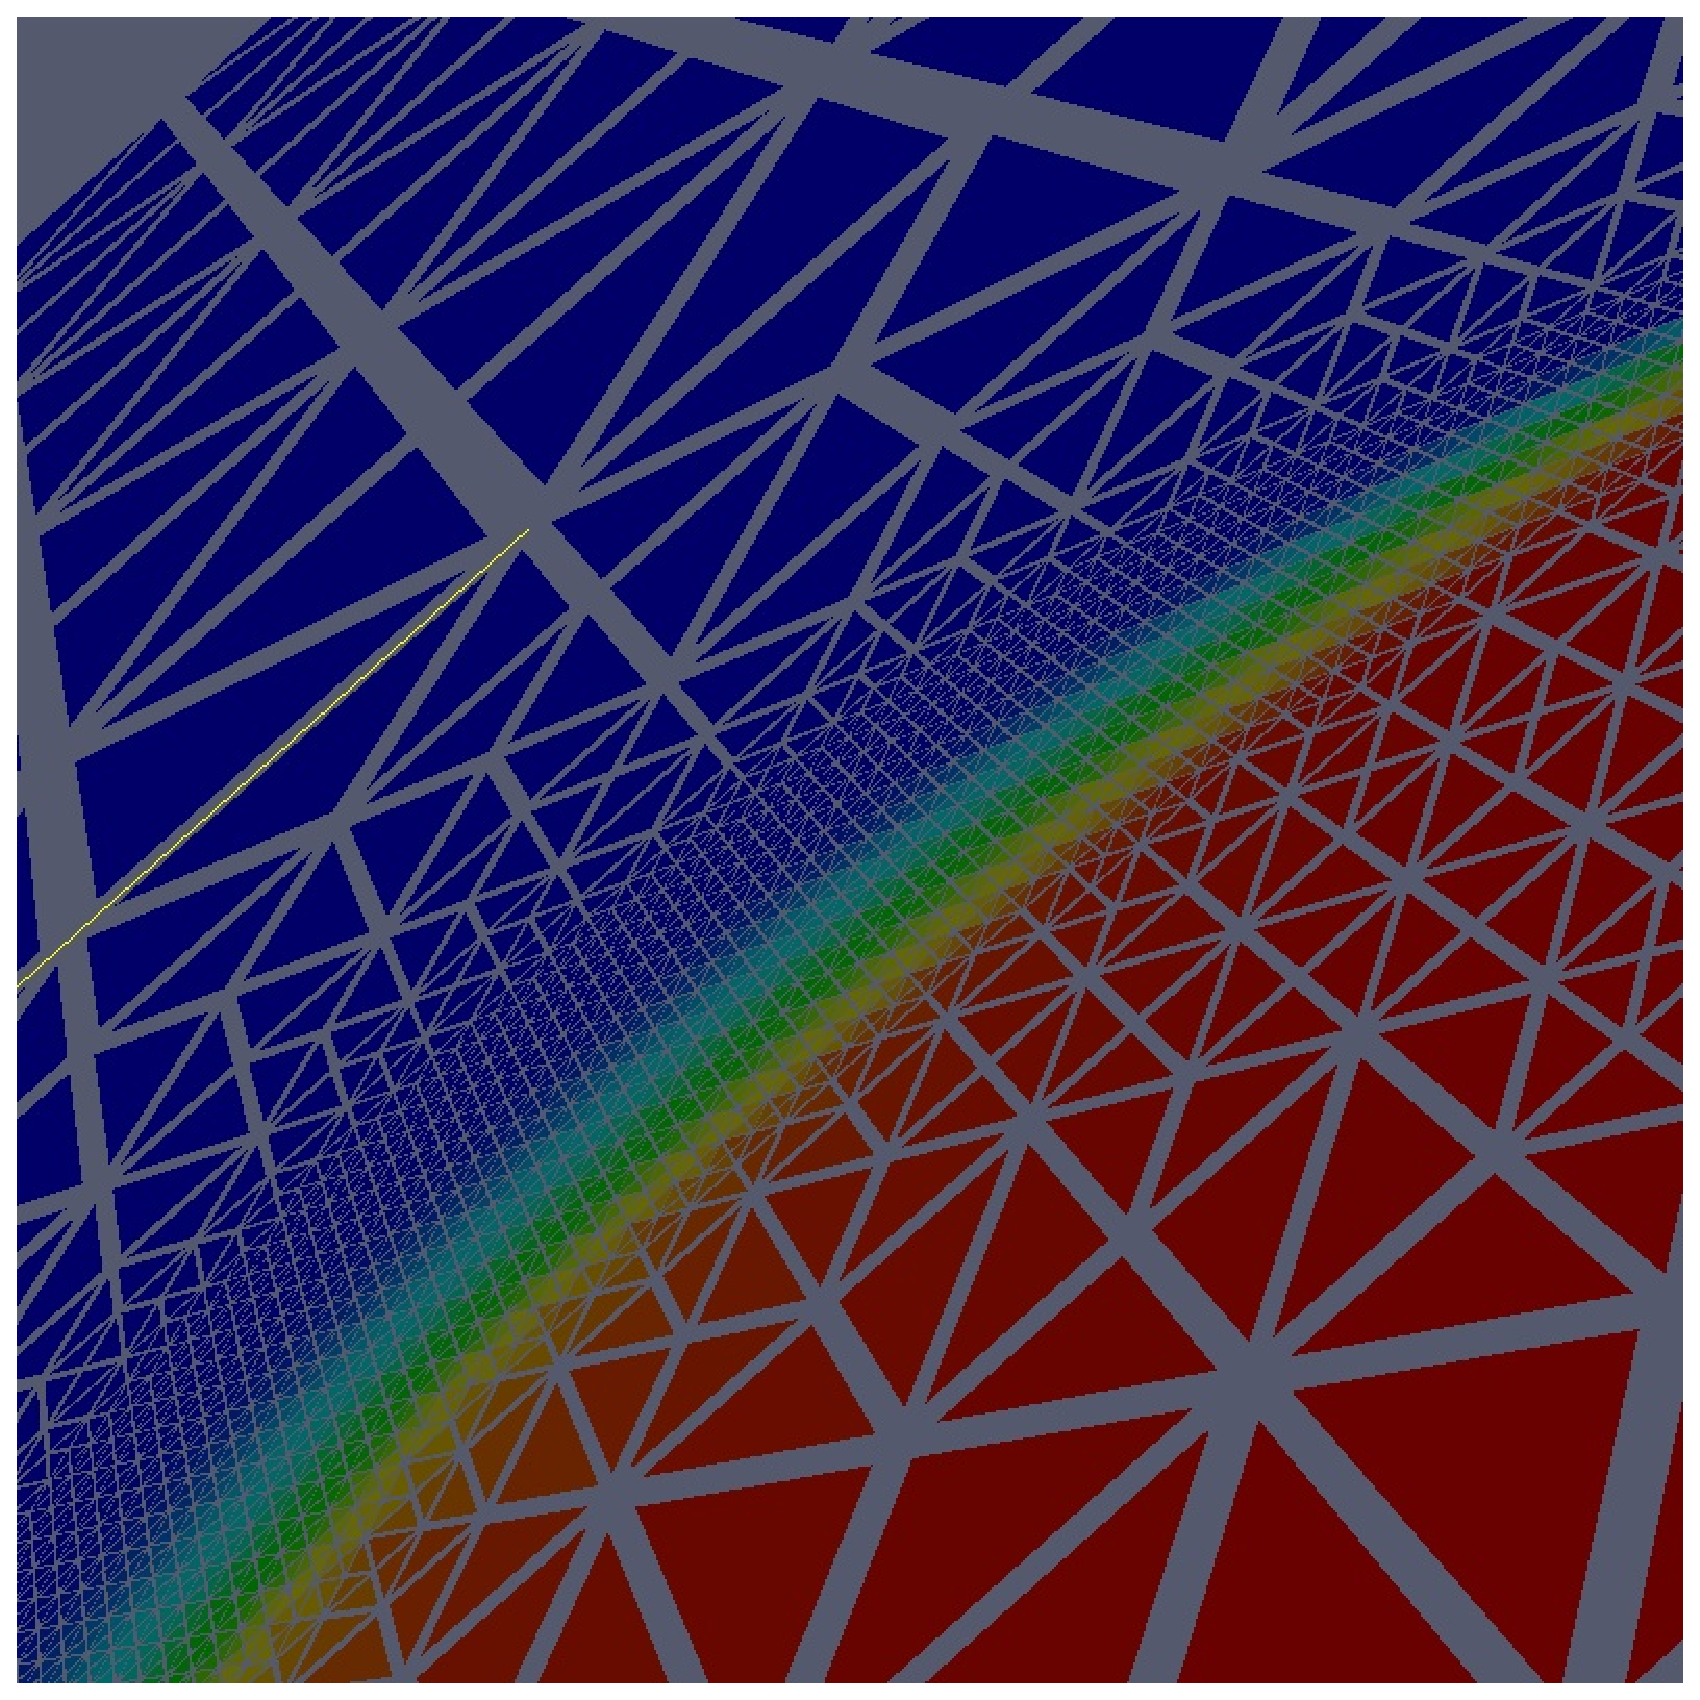
\includegraphics[width=0.32\textwidth]{EPS/alberta2d-view2}\hfill
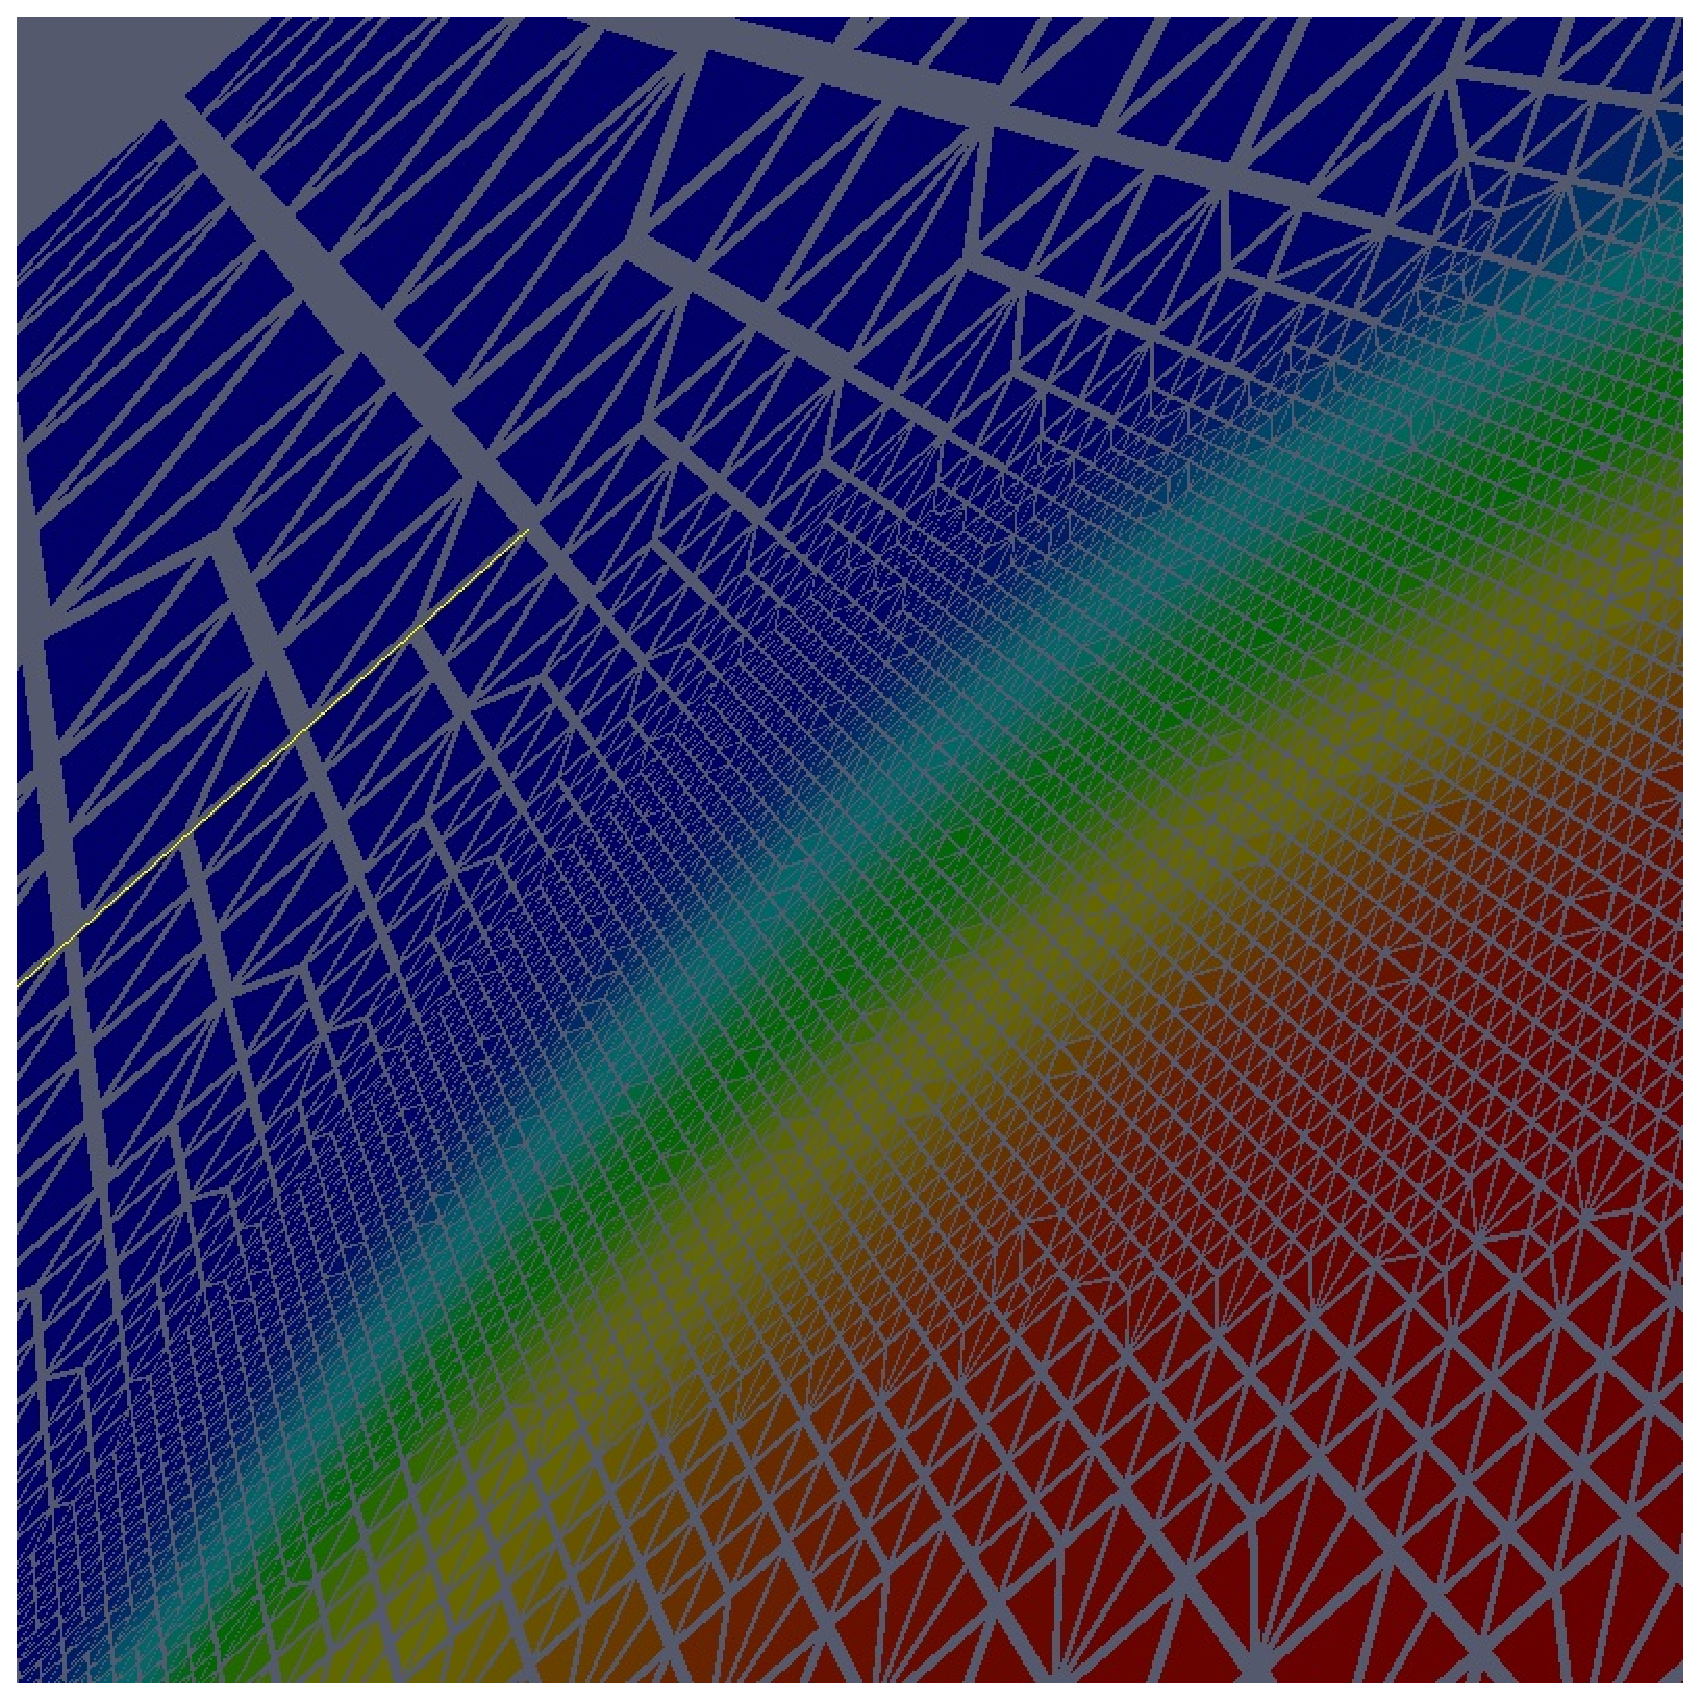
\includegraphics[width=0.32\textwidth]{EPS/ug2dtri-view2}\hfill
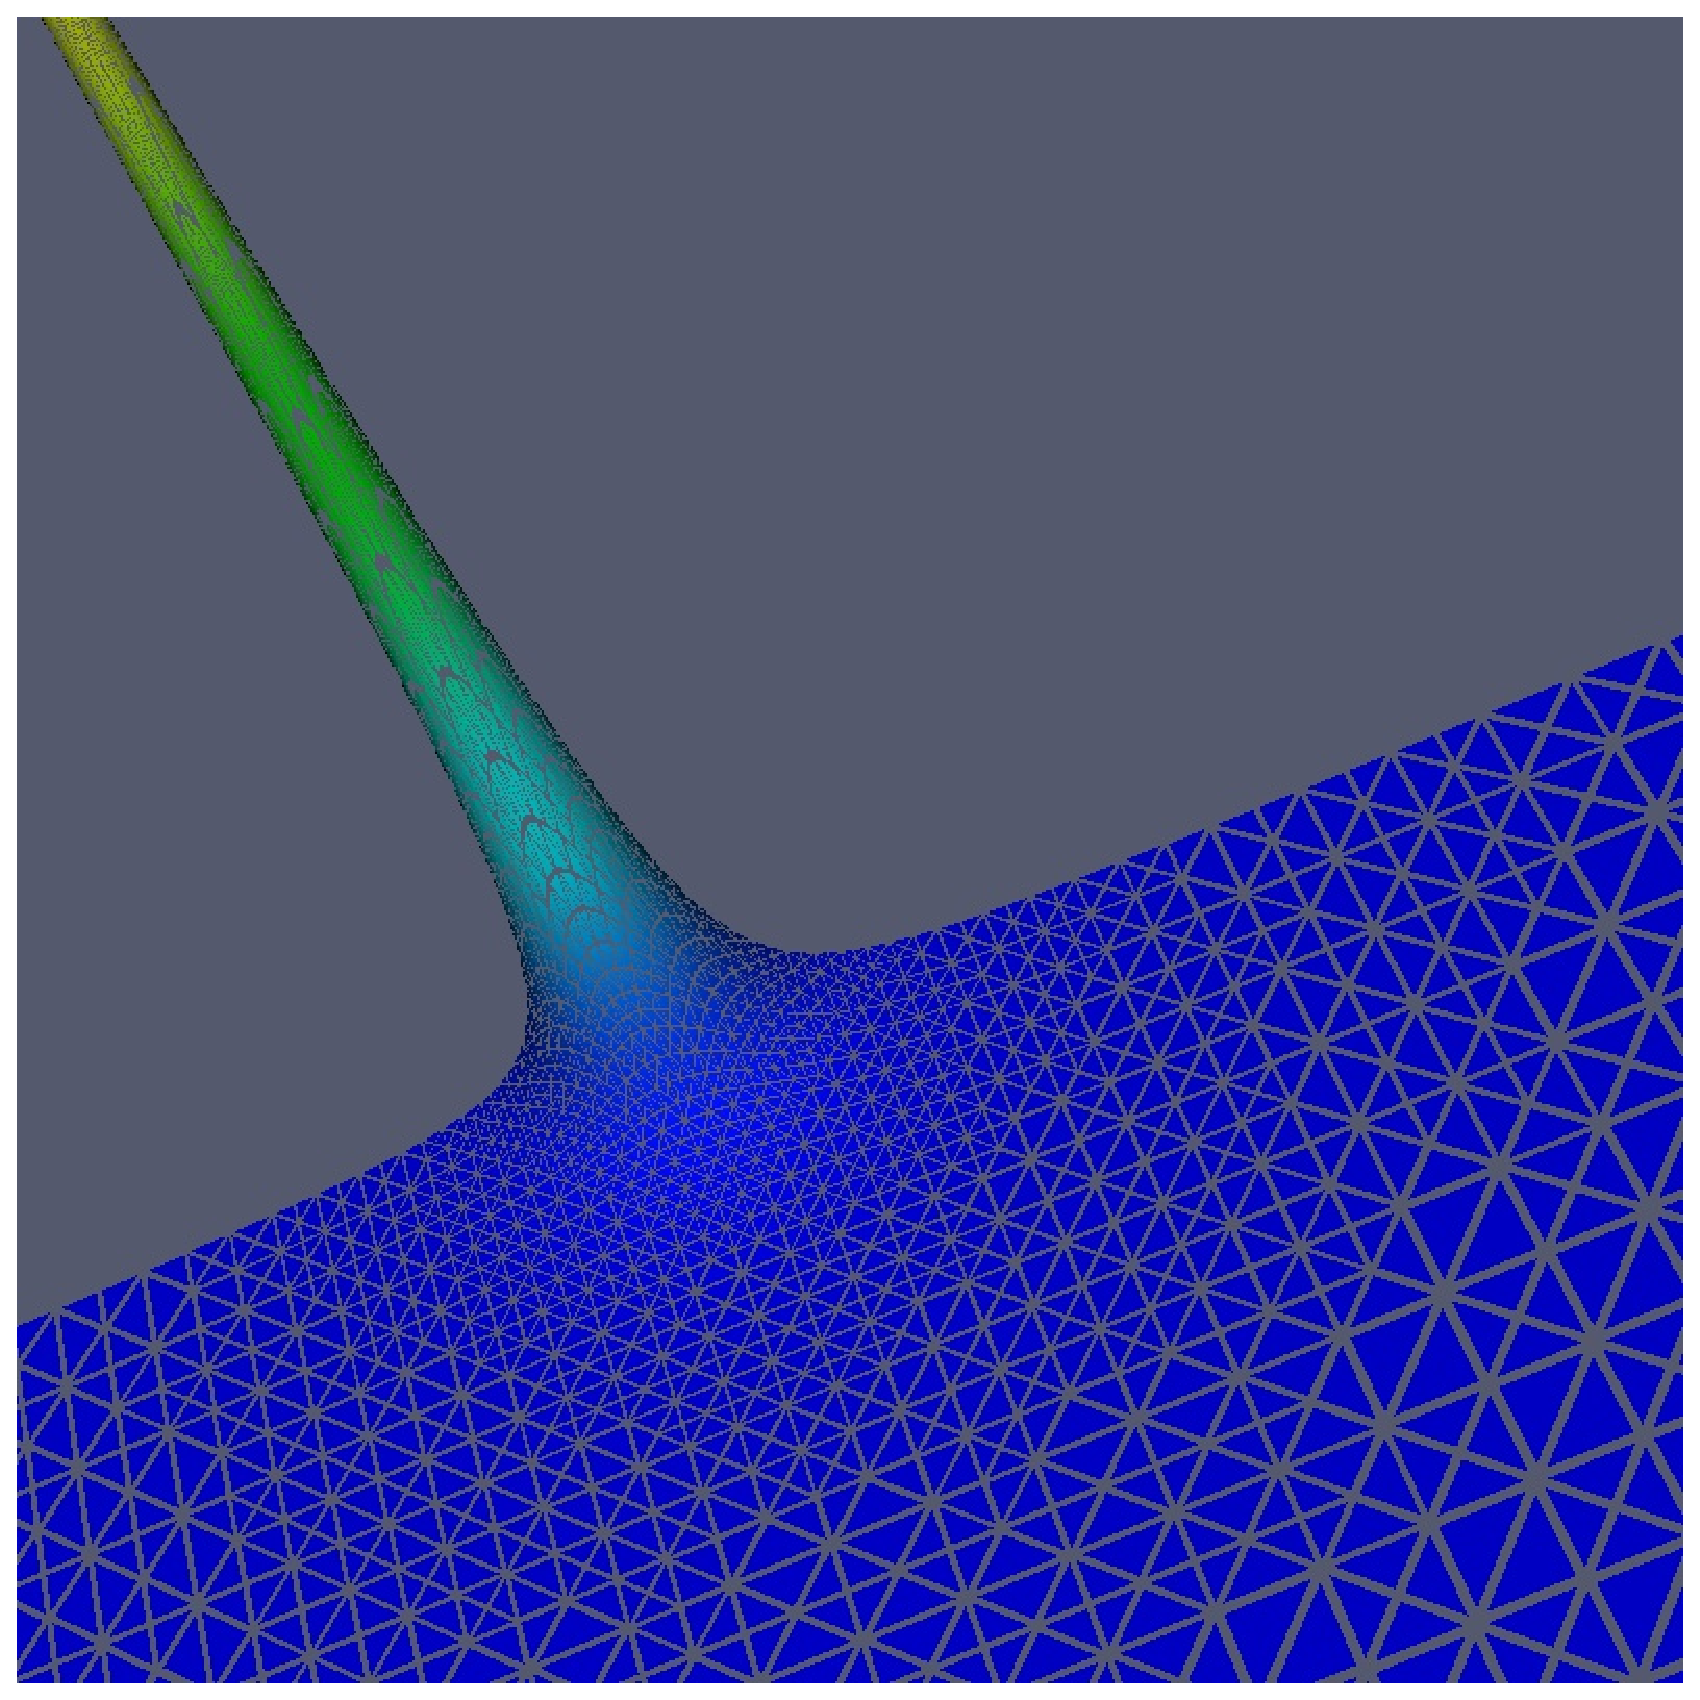
\includegraphics[width=0.32\textwidth]{EPS/adaptiveintegration_alberta2d}\hfill
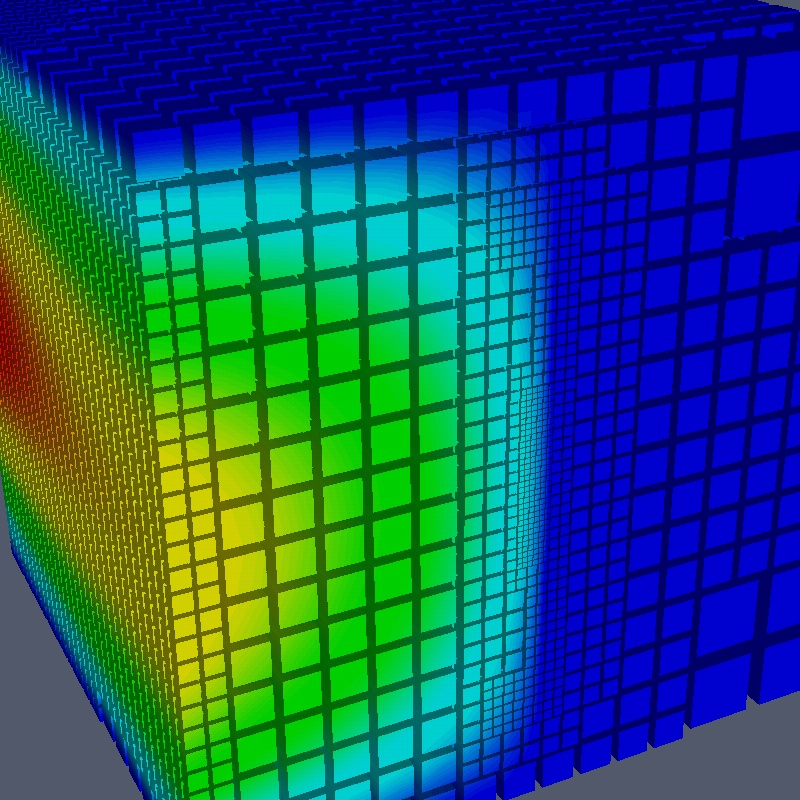
\includegraphics[width=0.32\textwidth]{EPS/alucube3d}
%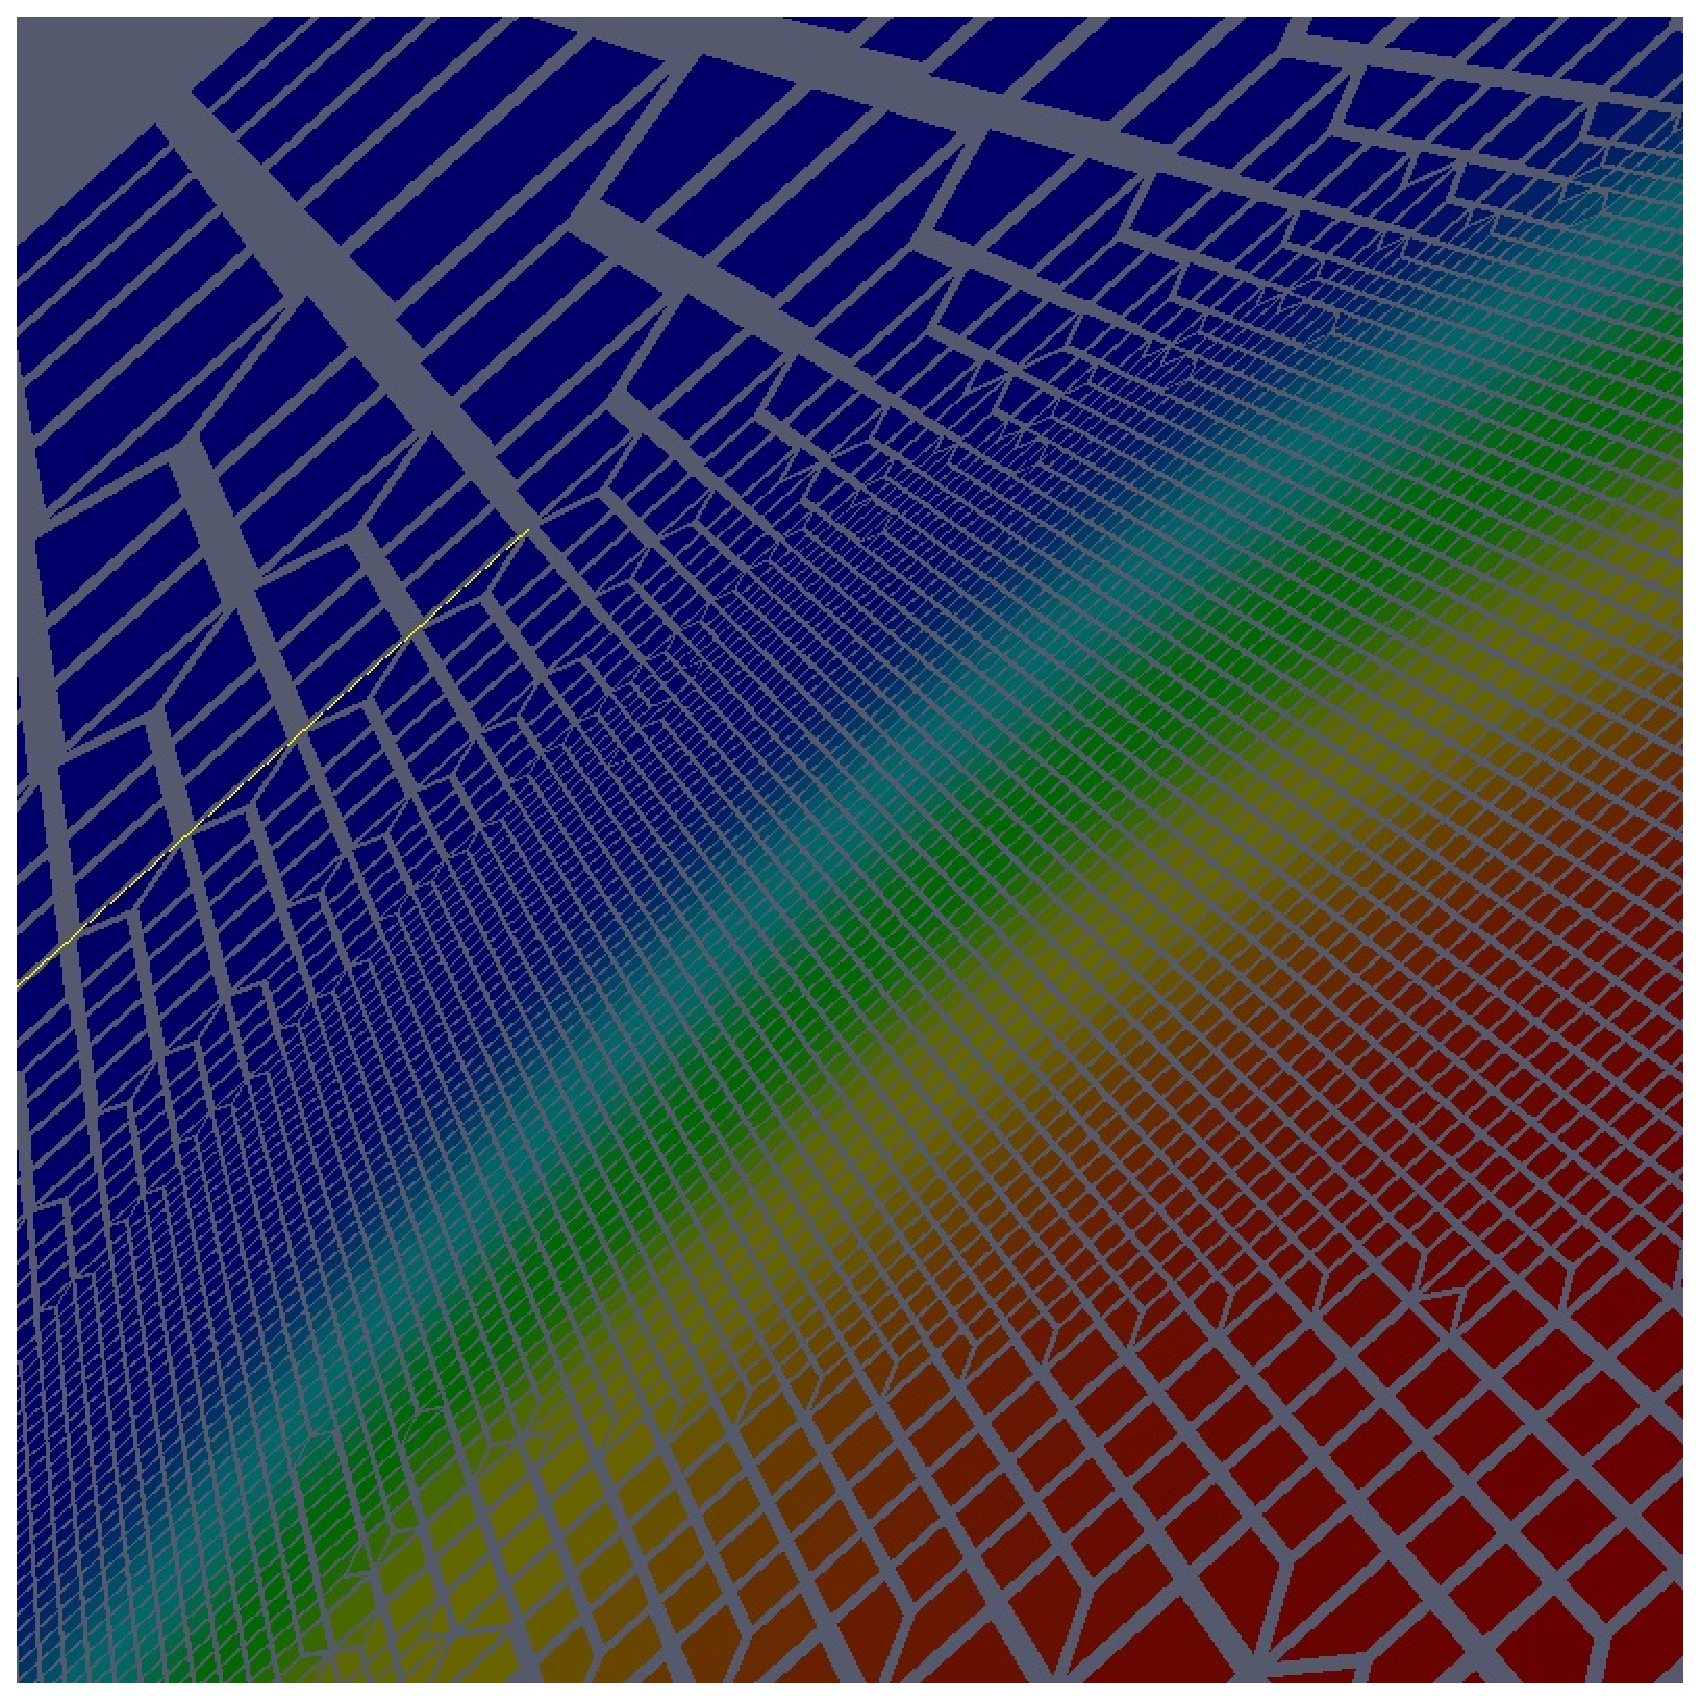
\includegraphics[width=0.32\textwidth]{EPS/ug2dquad-view2}
\\
\vspace{10mm}
{\normalsize $^\ast$Abteilung `Simulation gro\ss er Systeme',
Universit\"at Stuttgart,\\
Universit\"atsstr.~38, D-70569 Stuttgart, Germany}\\
%
\bigskip
{\normalsize $^\dagger$Abteilung f\"ur Angewandte Mathematik, Universit\"at Freiburg,\\
Hermann-Herder-Str.~10, D-79104 Freiburg, Germany}\\
%
\bigskip
{\normalsize $^\mathparagraph$Institut f\"ur Numerische und Angewandte Mathematik, Universit\"at M\"unster,\\
Einsteinstr.~62, D-48149 M\"unster, Germany}\\
%
\bigskip
{\normalsize $^\ddagger$Institut f\"ur Mathematik II,\\ Freie Universit\"at Berlin,
Arnimallee 6, D-14195 Berlin, Germany}\\
%
\bigskip
{\normalsize \texttt{\url{http://www.dune-project.org/}}}\\
}

\begin{document}

\maketitle

\begin{abstract}
This document gives an introduction to the Distributed and Unified
Numerics Environment (\Dune). \Dune{} is a template library for the
numerical solution of partial differential equations. It is based on
the following principles: i) Separation of data structures and
algorithms by abstract interfaces, ii) Efficient implementation of these
interfaces using generic programming techniques (templates) in C++ and
iii) Reuse of existing finite element packages with a large body of
functionality. This introduction covers only the abstract grid interface
of \Dune{} which is currently the most developed part. However, part of
\Dune{} are also the Iterative Solver Template Library (ISTL, providing a
large variety of solvers for sparse linear systems) and a flexible class
hierarchy for finite element methods. These will be described in
subsequent documents. Now have fun!

\vspace*{\fill}
Thanks to Martin Drohmann for adapting this howto to version 1.2 of the
DUNE grid interface.
\end{abstract}

\tableofcontents


%%%%%%%%%%%%%%%%%%%%%%%%%%%%%%%%%%%%%%%%%%%%%%%%%%%%%%%%%%%%%%%%%%%%%%%%%%%
%%%%%%%%%%%%%%%%%%%%%%%%%%%%%%%%%%%%%%%%%%%%%%%%%%%%%%%%%%%%%%%%%%%%%%%%%%%
\chapter{Introduction}
%%%%%%%%%%%%%%%%%%%%%%%%%%%%%%%%%%%%%%%%%%%%%%%%%%%%%%%%%%%%%%%%%%%%%%%%%%%
%%%%%%%%%%%%%%%%%%%%%%%%%%%%%%%%%%%%%%%%%%%%%%%%%%%%%%%%%%%%%%%%%%%%%%%%%%%

\section{What is \texorpdfstring{\Dune{}}{DUNE} anyway?}

\Dune{} is a software framework for the numerical solution of partial
differential equations with grid-based methods. It is based on the
following main principles:
\begin{itemize}
\item \textit{Separation of data structures and
algorithms by abstract interfaces.} This provides more functionality
with less code and also ensures maintainability and
extendability of the framework.
\item \textit{Efficient implementation of these
interfaces using generic programming techniques}. Static polymorphism
allows the compiler to do more optimizations, in particular function
inlining, which in turn allows the interface to have very small
functions (implemented by one or few machine instructions) without a
severe performance penalty. In essence the algorithms are parametrized
with a particular data structure and the interface is removed at
compile time. Thus the resulting code is as efficient as if it would
have been written for the special case.
\item \textit{Reuse of existing finite element packages with a large body of
functionality.} In particular the finite element codes UG, \cite{ug},
Alberta, \cite{Alberta}, and ALU3d, \cite{ALU3d}, have been
adapted to the \Dune{} framework. Thus, parallel and adaptive meshes with
multiple element types and refinement rules are available. All these
packages can be linked together in one executable.
\end{itemize}

The framework consists of a number of modules which are downloadable
as separate packages.  The current core modules are:
\begin{itemize}
\item \texttt{dune-common} contains the basic classes used by all
  \Dune{}-modules.  It provides some infrastructural classes for
  debugging and exception handling as well as a library to handle
  dense matrices and vectors.
\item \texttt{dune-geometry} provides element geometry classes and
  quadrature rules.
\item \texttt{dune-grid} is the grid interface and is covered in
  this document. It defines nonconforming, hierarchically nested,
  multi-element-type, parallel grids in arbitrary space dimensions.
  Graphical output with several packages is available, e.~g.~file
  output to VTK (parallel XML format for
  unstructured grids). The graphics package Grape, \cite{Grape} has
  been integrated in interactive mode.
\item \texttt{dune-istl} -- \textit{Iterative Solver Template
    Library.} Provides generic sparse matrix/vector classes and a
  variety of solvers based on these classes. A special feature is the
  use of templates to exploit the recursive block structure of finite
  element matrices at compile time. Available solvers include Krylov
  methods, (block-) incomplete decompositions and aggregation-based
  algebraic multigrid.
 \item \texttt{dune-localfunctions} -- \textit{Library of local base
  functions.} Provides classes for base functions on reference elements
  from which global discrete function spaces can be constructed.
\end{itemize}

Before starting to work with \Dune{} you might want to update your
knowledge about C++ and templates in particular. For that you should
have the bible, \cite{Stroustrup}, at your desk. A good introduction,
besides its age, is still the book by Barton and Nackman,
\cite{BN}. The definitive guide to template programming is
\cite{VandervoordeJosuttis}. A very useful compilation of template
programming tricks with application to scientific computing is given
in \cite{Veldhui99} (if you can't find it on the web, contact us).

\section{Download}

The source code of the \Dune{} framework can be
downloaded from the web page.  To get started, it is easiest to
download the latest stable version of the tarballs of
\texttt{dune-common}, \texttt{dune-grid} and \texttt{dune-grid-howto}.
These are available on the \Dune{} download page:
%
\begin{center}
\url{http://www.dune-project.org/download.html}
\end{center}
%

Alternatively, you can download the latest development version via
anonymous Git.  For further information, please see the web page.

\section{Installation}

The official installation instructions are available on the web page
%
\begin{center}
\url{http://www.dune-project.org/doc/installation-notes.html}
\end{center}

Obviously, we do not want to copy all this information because it might
get outdated and inconsistent then. To make this document
self-contained, we describe only how to install \Dune{} from the
tarballs.  If you prefer to use the version from Git, see the web page
for further information.  Moreover, we assume that you use a UNIX
system (usually Linux or OS X). If you have the Redmond system then
you have to explore new horizons.

In order to build the \Dune{} framework, you need a standards
compliant C++ compiler.  We tested compiling with GNU \texttt{g++} in
version 4.4 or newer and \texttt{clang} in version 3.4 or newer. Recent versions
of Intel \texttt{icc} ($\geq 15$) should work, too. For older versions of
\texttt{icc}, like $14.0.3$, several issues are known and usage of these
is discouraged.

Now extract the tarballs of \texttt{dune-common},
\texttt{dune-geometry}, \texttt{dune-istl}, \texttt{dune-grid},
and \texttt{dune-grid\-howto} into a common directory, say
\texttt{dune-home}.  Change to this directory and call
\begin{lstlisting}
> dune-common-2.3/bin/dunecontrol all
\end{lstlisting}
Replace ``\texttt{2.3}'' by the actual version number of the package
you downloaded if necessary.  This should configure and build all
\Dune{} modules in \texttt{dune-home} with a basic configuration.

For many of the examples in this howto you need adaptive grids or the
parallel features of \Dune{}.  To use adaptive grids, you need to
install one of the external grid packages which \Dune{} provides
interfaces for, for instance Alberta, UG and ALUGrid.
\begin{itemize}
\item Alberta -- \url{http://www.alberta-fem.de/}
\item UG -- \url{http://www.iwr.uni-heidelberg.de/frame/iwrwikiequipment/software/ug}
\item \Dune{}-ALUGrid -- \url{http://users.dune-project.org/projects/dune-alugrid}
\end{itemize}
To use the parallel code of \Dune{}, you need an implementation of the
Message Passing Interface (MPI), for example MPICH or Open MPI.  For the
\Dune{} build system to find these libraries, the \texttt{configure}
scripts of the particular \Dune{} modules must be passed the locations
of the respective installations.  The \texttt{dunecontrol} script
facilitates to pass options to the \texttt{configure} via a
configuration file.  Such a configuration file might look like this:
\begin{lstlisting}
CONFIGURE_FLAGS="--with-alberta=/path/to/alberta "\
"--with-ug=/path/to/ug --enable-parallel"
MAKE_FLAGS="-j 2"
\end{lstlisting}
If this is saved under the name \texttt{dunecontrol.opts}, you
can tell \texttt{dunecontrol} to consider the file by calling
\begin{lstlisting}
> dune-common-2.3/bin/dunecontrol --opts=dunecontrol.opts all
\end{lstlisting}

For information on how to build and configure the respective grids,
please see the \Dune{} web page.

\section{Code documentation}

Documentation of the files and classes in \Dune{} is provided in code and
can be extracted using the
Doxygen\footnote{\url{http://www.doxygen.org/}}
software available elsewhere. The code documentation can either be built
locally on your machine (in HTML and other formats, e.\,g.~\LaTeX)
or its latest version is available at
\begin{center}
\url{http://www.dune-project.org/doc/doxygen.html}
\end{center}

\section{Licence}

The \Dune{} library and headers are licensed under version 2 of the
GNU General Public License%
\footnote{\url{http://www.gnu.org/licenses/gpl-2.0.html}}, with a special
exception for linking and compiling against \Dune{}, the so-called
``runtime exception.''  The license is intended to be similar to the
GNU Lesser General Public License, which by itself isn't suitable for
a C++ template library.

The exact wording of the exception reads as follows:

\begin{quote}
   As a special exception, you may use the \Dune{} source files as part
   of a software library or application without restriction.
   Specifically, if other files instantiate templates or use macros or
   inline functions from one or more of the \Dune{} source files, or you
   compile one or more of the \Dune{} source files and link them with
   other files to produce an executable, this does not by itself cause
   the resulting executable to be covered by the GNU General Public
   License.  This exception does not however invalidate any other
   reasons why the executable file might be covered by the GNU General
   Public License.
\end{quote}

%\section{Contributing to DUNE}




%%%%%%%%%%%%%%%%%%%%%%%%%%%%%%%%%%%%%%%%%%%%%%%%%%%%%%%%%%%%%%%%%%%%%%%%%%%
%%%%%%%%%%%%%%%%%%%%%%%%%%%%%%%%%%%%%%%%%%%%%%%%%%%%%%%%%%%%%%%%%%%%%%%%%%%
\chapter{Getting started}
%%%%%%%%%%%%%%%%%%%%%%%%%%%%%%%%%%%%%%%%%%%%%%%%%%%%%%%%%%%%%%%%%%%%%%%%%%%
%%%%%%%%%%%%%%%%%%%%%%%%%%%%%%%%%%%%%%%%%%%%%%%%%%%%%%%%%%%%%%%%%%%%%%%%%%%

In this section we will take a quick tour through the abstract
grid interface provided by \Dune. This should give you an overview of
the different classes before we go into the details.

\section{Creating your first grid}

Let us start with a replacement of the famous \emph{hello world}
program given below.

\begin{lst}[File dune-grid-howto/gettingstarted.cc] \mbox{}
\lstinputlisting[basicstyle=\ttfamily\scriptsize,numbers=left,
numberstyle=\tiny, numbersep=5pt]{../gettingstarted.cc}
\end{lst}

This program is quite simple. It starts with some includes in lines
\ref{gs:inc0}-\ref{gs:inc1}. The file \lstinline!config.h! has been
produced by the \lstinline!configure! script in the application's
build system. It contains the current configuration and can be used to
compile different versions of your code depending on the configuration
selected. It is important that this file is included before any other
\Dune{} header files. The file \lstinline!dune/grid/yaspgrid.hh!
includes the headers for the \lstinline!YaspGrid! class which provides a
special implementation of the \Dune{} grid interface with a
structured mesh of arbitrary dimension. Then
\lstinline!dune/grid/common/gridinfo.hh!  loads the headers of some
functions which print useful information about a grid.

Since the dimension will be used as a template parameter in many
places below we define it as a constant in line number \ref{gs:dim}.
The \lstinline!YaspGrid! class template takes its dimension as a
template parameter.  Technically, \lstinline!YaspGrid! has a second template
parameter, that defines how it stores coordinates. In this example, we
use an equidistant grid, which allows us to stay with the default value
\lstinline!EquidistantCoordinates!. For ease of writing we
define in line \ref{gs:gridtype} the type \lstinline!GridType! using
the selected value for the dimension. All identifiers of the \Dune{}
framework are within the \lstinline!Dune! namespace.

Lines \ref{gs:par0}-\ref{gs:par1} prepare the arguments for the
construction of a \lstinline!YaspGrid! object. The first argument use
the class template \lstinline!FieldVector<T,n>! which is a vector with
\lstinline!n!  components of type \lstinline!T!. You can either assign
the same value to all components in the constructor (as is done here)
or you could use \lstinline!operator[]! to assign values to individual
components. The variable \lstinline!length! defines the lengths of
the cube. The variable \lstinline!elements! defines the number of
cells or elements to be used in the respective dimension of the grid.
Finally in line \ref{gs:grid} we are now able to
instantiate the \lstinline!YaspGrid!  object.

The only thing we do with the grid in this little example is printing
some information about it. After successfully running the executable
\lstinline!gettingstarted! you should see an output like this:

\begin{lst}[Output of gettingstarted] \mbox{}

\begin{lstlisting}[basicstyle=\ttfamily\scriptsize]
=> Dune::YaspGrid<3, Dune::EquidistantCoordinates<double, 3> > (dim=3, dimworld=3)
level 0 codim[0]=64 codim[1]=240 codim[2]=300 codim[3]=125
leaf    codim[0]=64 codim[1]=240 codim[2]=300 codim[3]=125
leaf dim=3 geomTypes=((cube, 3)[0]=64,(cube, 2)[1]=240,(simplex, 1)[2]=300,(simplex, 0)[3]=125)
\end{lstlisting}
\end{lst}

The first line tells you that you are looking at an \lstinline!YaspGrid!
object of the given dimensions. The \Dune{} grid interface supports
unstructured, locally refined, logically nested grids. The coarsest
grid is called level-0-grid or macro grid. Elements can be
individually refined into a number of smaller elements. Each element
of the macro grid and all its descendants obtained from refinement
form a tree structure. All elements at depth $n$ of a refinement tree
form the level-$n$-grid. All elements that are leaves of a refinement
tree together form the so-called leaf grid. The second line of the
output tells us that this grid object consists only of a single level
(level $0$) while the next line tells us that that level 0 coincides
also with the leaf grid in this case. Each line reports about the
number of grid entities which make up the grid. We see that there are
64 elements (codimension 0), 240 faces (codimension 1), 300 edges
(codimension 2) and 125 vertices (codimension 3) in the grid. The last
line reports on the different types of entities making up the grid. In
this case all entities are of type \emph{cube}, as a line and a point
are both \emph{cube} and \emph{simplex}.

\begin{exc} Try to play around with different grid sizes by assigning
  different values to the \lstinline!element! parameter. You can also change
  the dimension of the grid by varying \lstinline!dim!. Don't be
  modest. Also try dimensions 4 and 5!
\end{exc}

\begin{exc}
  The static methods \lstinline!Dune::gridlevellist! and
  \lstinline!Dune::gridleaflist! produce a very detailed output of the grid's
  elements on a specified grid level. Change the code and print out this
  information for the leaf grid or a grid on lower level. Try to understand the
  output.
\end{exc}

\section{Traversing a grid --- A first look at the grid interface}

After looking at very first simple example we are now ready to go on
to a more complicated one. Here it is:

\begin{lst}[File dune-grid-howto/traversal.cc] \mbox{}
\nopagebreak
\lstinputlisting[basicstyle=\ttfamily\scriptsize,numbers=left,
numberstyle=\tiny, numbersep=5pt]{../traversal.cc}
\end{lst}

The \lstinline!main! function near the end of the listing is pretty
similar to the previous one except that we use a 2d grid for the unit
square that just consists of one cell. In line \ref{tc:refine} this
cell is refined once using the standard method of grid refinement of
the implementation. Here, the cell is refined into four smaller cells.
The main work is done in a call to the function \lstinline!traversal!
in line \ref{tc:call}.  This function is given in lines
\ref{tc:tra0}-\ref{tc:tra1}.

The function \lstinline!traversal! is a function template that is
parametrized by a class \lstinline!G! that is assumed to implement
the \Dune{} grid interface.  Thus, it will work on \textit{any} grid
available in \Dune{} without any changes. We now go into the details
of this function.

The algorithm should work in any dimension so we extract the grid's
dimension in line \ref{tc:dim}. Next, each \Dune{} grid defines a type
that it uses to represent positions. This type is extracted in line
\ref{tc:ct} for later use.

A grid is considered to be a container of ``entities'' which are
abstractions for geometric objects like vertices, edges,
quadrilaterals, tetrahedra, and so on. This is very similar to the
standard template library (STL), see e.~g.~\cite{Stroustrup},
which is part of any C++ system.
A key difference is, however, that there is not just one type of entity but
several. As in the STL the elements of any container can be accessed
with iterators which are generalized pointers. Again, a \Dune{} grid
knows several different iterators which provide access to the
different kinds of entities and which also provide different patterns
of access.

As we usually do not want to use the entire hierarchy of the grid, we first
define a view on that part of the grid we are interested in. This can be a
level or the leaf part of the grid. In line \ref{tc:lfgv} a type for a
\lstinline!GridView! on the leaf grid is defined.

Line \ref{tc:ittype} extracts the type of an iterator from this view
class. \lstinline!Codim! is a \lstinline!struct! within the grid class
that takes an integer template parameter specifying the codimension
over which to iterate. Within the \lstinline!Codim! structure the type
\lstinline!Iterator! is defined. Since we specified codimension 0
this iterator is used to iterate
over the elements which are not refined any further, i.e.~which are
the leaves of the refinement trees.

The \lstinline!for!-loop in line \ref{tc:forel} now visits every such
element. The \lstinline!begin! and \lstinline!end! on the
\lstinline!LeafGridView!
class deliver the first leaf element and one past the last leaf element. Note
that the \lstinline!template! keyword must be used and template parameters are
passed explicitly. Within the loop body in
lines \ref{tc:forel0}-\ref{tc:forel1} the iterator \lstinline!it! acts
like a pointer to an entity of dimension \lstinline!dim! and
codimension 0. The exact type would be
\lstinline!typename G::template Codim<0>::Entity! just to mention it.

Please note, that from Dune 2.4 on, C++11 range based for statements will
be used to iterate over entities of a grid. To enable this feature, you will
need \texttt{g++} version 4.6 or higher. There are no issues with the mentioned
version of \texttt{icc} or \texttt{clang}. The entire iteration loop,
will then boil down to
\begin{lstlisting}[basicstyle=\ttfamily\scriptsize,numbers=left,
numberstyle=\tiny, numbersep=5pt]
 for (auto&& e : elements(leafView))
 {
   // the iteration loop
 }
\end{lstlisting}

There is no more need of getting the iterator type by hand. Note that you
should always write \lstinline!auto&&! !In contrast to the above procedure you don't
get an \lstinline!EntityPointer!, but a reference to the \lstinline!Entity!
itself.

An important part of an entity is its geometrical shape and position.
All geometrical information is factored out into a sub-object that can
be accessed via the \lstinline!geometry()!  method. The geometry
object is in general a mapping from a $d$-dimensional polyhedral
reference element to $w$ dimensional space. Here we have $d=$
\lstinline!G::dimension! and $w=$ \lstinline!G::dimensionworld!. This
mapping is also called the ``local to global'' mapping.  The
corresponding reference element has a certain type which is extracted
in line \ref{tc:reftype}. Since the reference elements are polyhedra
they consist of a finite number of corners. The images of the corners
under the local to global map can be accessed via the
\lstinline!corner(int n)! method. Line \ref{tc:print} prints the geometry type
and the position of the first corner of the element. Then line
\ref{tc:count} just counts the number of elements visited.

Suppose now that we wanted to iterate over the vertices of the leaf
grid instead of the elements. Now vertices have the codimension
\lstinline!dim! in a \lstinline!dim!-dimensional grid and a
corresponding iterator is provided by each grid class. It is extracted
in line \ref{tc:vertit} for later use. The \lstinline!for!-loop
starting in line \ref{tc:forve} is very similar to the first one
except that it now uses the \lstinline!VertexLeafIterator!.  As you
can see the different entities can be accessed with the same methods.
We will see later that codimensions 0 and \lstinline!dim! are
specializations with an extended interface compared to all other
codimensions. You can also access the codimensions between 0 and
\lstinline!dim!. However, currently not all implementations of the
grid interface support these intermediate codimensions (though this
does not restrict the implementation of finite element methods with
degrees of freedom associated to, say, faces).

Again, above task, can be done with a range based for statement by
using the function \lstinline!vertices! instead of \lstinline!elements!
in the above code snippet.

Finally, we show in lines \ref{tc:level0}-\ref{tc:level1} how the
hierarchic structure of the mesh can be accessed. To that end a
\lstinline!LevelGridView! is used. It provides via an \lstinline!Iterator!
access to all entities of a given codimension (here 0) on a given grid level.
The coarsest
grid level (the initial macro grid) has number zero and the number of
the finest grid level is returned by the \lstinline!maxLevel()! method
of the grid.  The methods \lstinline!begin()! and \lstinline!end()!
on the view deliver iterators to the first and one-past-the-last
entity of a given grid level supplied as an integer argument to these
methods.

The following listing shows the output of the program.

\begin{lst}[Output of traversal] \mbox{}

\begin{lstlisting}[basicstyle=\ttfamily\scriptsize]
*** Traverse codim 0 leaves
visiting leaf (cube, 2) with first vertex at -1 -1
visiting leaf (cube, 2) with first vertex at 0 -1
visiting leaf (cube, 2) with first vertex at -1 0
visiting leaf (cube, 2) with first vertex at 0 0
there are/is 4 leaf element(s)

*** Traverse codim 2 leaves
visiting (cube, 0) at -1 -1
visiting (cube, 0) at 0 -1
visiting (cube, 0) at 1 -1
visiting (cube, 0) at -1 0
visiting (cube, 0) at 0 0
visiting (cube, 0) at 1 0
visiting (cube, 0) at -1 1
visiting (cube, 0) at 0 1
visiting (cube, 0) at 1 1
there are/is 9 leaf vertices(s)

*** Traverse codim 0 level-wise
visiting (cube, 2) with first vertex at -1 -1
there are/is 1 element(s) on level 0

visiting (cube, 2) with first vertex at -1 -1
visiting (cube, 2) with first vertex at 0 -1
visiting (cube, 2) with first vertex at -1 0
visiting (cube, 2) with first vertex at 0 0
there are/is 4 element(s) on level 1
\end{lstlisting}
\end{lst}

\begin{rem} Define the end iterator for efficiency.
\end{rem}

\begin{exc} Play with different dimensions, codimension
  (\lstinline!YaspGrid! supports all codimenions) and refinements.
\end{exc}

\begin{exc} The method \lstinline!corners()! of the geometry returns
  the number of corners of an entity. Modify the code such that the
  positions of all corners are printed.
\end{exc}


%%%%%%%%%%%%%%%%%%%%%%%%%%%%%%%%%%%%%%%%%%%%%%%%%%%%%%%%%%%%%%%%%%%%%%%%%%%
%%%%%%%%%%%%%%%%%%%%%%%%%%%%%%%%%%%%%%%%%%%%%%%%%%%%%%%%%%%%%%%%%%%%%%%%%%%
\chapter{The \texorpdfstring{\Dune{}}{DUNE} grid interface}
%%%%%%%%%%%%%%%%%%%%%%%%%%%%%%%%%%%%%%%%%%%%%%%%%%%%%%%%%%%%%%%%%%%%%%%%%%%
%%%%%%%%%%%%%%%%%%%%%%%%%%%%%%%%%%%%%%%%%%%%%%%%%%%%%%%%%%%%%%%%%%%%%%%%%%%


\section{Grid definition}

There is a great variety of grids: conforming and non-conforming
grids, single-element-type and multiple-element-type grids, locally
and globally refined grids, nested and non-nested grids,
bisection-type grids, red-green-type grids, sparse grids and so on. In
this section we describe in some detail the type of grids that are
covered by the \Dune{} grid interface.

\minisec{Reference elements}

A computational grid is a non-overlapping subdivision of a domain
$\Omega\subset\R^w$ into elements of ``simple'' shape. Here ``simple''
means that the element can be represented as the image of a reference
element under a transformation. A reference element is a convex
polytope, which is a bounded intersection of a finite set of
half-spaces.

\minisec{Dimension and world dimension}

A grid has a dimension $d$ which is the dimensionality of
its reference elements. Clearly we have $d\leq w$. In the case $d<w$ the grid
discretizes a $d$-dimensional manifold.

\minisec{Faces, entities and codimension}

The intersection of a $d$-dimensional convex polytope (in
$d$-dimensional space) with a
tangent plane is called a face (note that there are faces of
dimensionality $0,\ldots,d-1$). Consequently, a face of a grid element
is defined as the image of a face of its reference element under the
transformation. The elements and faces of elements of a grid are
called its entities. An entity is said to be of codimension $c$ if it
is a $d-c$-dimensional object. Thus the elements of the grid are
entities of codimension 0, facets of an element have codimension 1,
edges have codimension $d-1$ and vertices have codimension $d$.

\minisec{Conformity}

Computational grids come in a variety of flavours: A
{conforming} grid is one where the intersection of two
elements is either empty or a face of each of the two elements.
Grids where the intersection of two elements may have an
arbitrary shape are called {nonconforming}.

\minisec{Element types}

A {simplicial} grid is one where the reference elements are
simplices. In a {multi-element-type} grid a finite number of
different reference elements are allowed. The \Dune{} grid interface
can represent conforming as well as non-conforming grids.

\minisec{Hierarchically nested grids, macro grid}

A {hierarchically nested} grid consists of a collection of $J+1$
grids that are subdivisions of nested domains $$\Omega=\Omega_0 \supseteq \Omega_1 \supseteq
\ldots \supseteq \Omega_J.$$ Note that only $\Omega_0$ is required to
be identical to $\Omega$. If $\Omega_0=\Omega_1=\ldots=\Omega_J$ the
grid is {globally refined}, otherwise it is {locally refined}.
The grid that discretizes $\Omega_0$ is called the macro grid and its
elements the macro elements. The
grid for $\Omega_{l+1}$ is obtained from the grid
for $\Omega_l$ by possibly subdividing each of its elements into
smaller elements. Thus, each element of the macro grid and the
elements that are obtained from refining it form a tree structure. The
grid discretizing $\Omega_l$ with $0\leq l \leq J$ is called the level-$l$-grid and its
elements are obtained from an $l$-fold refinement of some macro elements.

\minisec{Leaf grid}

Due to the nestedness of the domains we can partition the domain
$\Omega$ into $$\Omega = \Omega_J \cup \bigcup_{l=0}^{J-1}
\Omega_l\setminus\Omega_{l+1}.$$ As a consequence of the hierarchical
construction a computational grid discretizing $\Omega$ can be
obtained by taking the elements of the level-$J$-grid plus
the elements of the level-$J-1$-grid in the region
$\Omega_{J-1}\setminus\Omega_{J}$ plus the elements of the level-$J-2$-grid in the region
$\Omega_{J-2}\setminus\Omega_{J-1}$ and so on plus the elements of the level-$0$-grid in the region
$\Omega_{0}\setminus\Omega_{1}$. The grid resulting from this
procedure is called the leaf grid
because it is formed by the leaf elements of the trees emanating at
the macro elements.

\minisec{Refinement rules}

There is a variety of ways how to hierarchically refine a grid. The
refinement is called conforming if the leaf grid is always a
conforming grid, otherwise the refinement is called
non-conforming. Note that the grid on each level $l$ might be
conforming while the leaf grid is not.
There are also many ways how to subdivide an individual element into
smaller elements. Bisection always subdivides elements into two
smaller elements, thus the resulting data structure is a binary tree
(independent of the dimension of the grid). Bisection is sometimes
called ``green'' refinement. The so-called ``red'' refinement is the
subdivision of an element into $2^d$ smaller elements, which is most
obvious for cube elements. In many practical situation anisotropic
refinement, i.~e.~refinement in a preferred direction, may be required.

\minisec{Summary}

The \Dune{} grid interface is able to represent grids with the
following properties:
\begin{itemize}
\item Arbitrary dimension.
\item Entities of all codimensions.
\item Any kind of reference elements (you could define the icosahedron
  as a reference element if you wish).
\item Conforming and non-conforming grids.
\item Grids are always hierarchically nested.
\item Any type of refinement rules.
\item Conforming and non-conforming refinement.
\item Parallel, distributed grids.
\end{itemize}



\section{Concepts}

Generic algorithms are based on concepts. A concept is a kind of
``generalized'' class with a well defined set of members.
Imagine a function template that takes a type \lstinline!T!
as template argument. All the members of \lstinline!T!, i.e.
methods, enumerations, data (rarely) and nested
classes  used by the function template form the concept. From that
definition it is clear that the concept does not necessarily exist as
program text.

A class that implements a concept is called a
\textit{model} of the concept. E.\,g.~in the standard template library (STL)
the class \lstinline!std::vector<int>! is a model of the concept
``container''. If all instances of a class template are a model of
a given concept we can also say that the class template is a model of
the concept. In that sense \lstinline!std::vector! is also a model of
container.

In standard OO language a concept would be formulated as
an abstract base class and all the models would be implemented as
derived classes. However, for reasons of efficiency we do not want to
use dynamic polymorphism. Moreover, concepts are more powerful because
the models of a concept can use different types, e.\,g.~as return types of
methods. As an example consider the STL where the begin method on a
vector of int returns \lstinline!std::vector<int>::iterator! and on a
list of int it returns \lstinline!std::list<int>::iterator! which may
be completely different types.

Concepts are difficult to describe when they do not exist as concrete
entities (classes or class templates) in a program. The STL way of
specifying concepts is to describe the members \lstinline!X::foo()! of
some arbitrary model named \lstinline!X!. Since this decription of the
concept is not processed by the compiler it can get inconsistent and
there is no way to check conformity of a model to the interface. As a
consequence, strange error messages from the compiler may be the
result (well C++ compilers can always produce strange error messages).
There are two ways to improve the situation:
\begin{itemize}
\item \textit{Engines:} A class template is defined that wraps the
  model (which is the template parameter) and forwards all member
  function calls to it. In addition all the nested types and
  enumerations of the model are copied into the wrapper class.
  The model can be seen as an engine that powers the wrapper class,
  hence the name. Generic
  algorithms are written in terms of the wrapper class. Thus the
  wrapper class encapsulates the concept and it can be ensured
  formally by the compiler that
  all members of the concept are implemented.

\item \textit{Barton-Nackman trick:} This is a refinement of the
  engine approach where the models are derived from the wrapper class
  template in addition. Thus static polymorphism is combined
  with a traditional class hierarchy, see \cite{Veldhui99,BN}.
  However, the
  Barton-Nackman trick gets rather involved when the derived classes
  depend on additional template parameters and several types are related
  with each other. That is why it is not used at all places in \Dune.
\end{itemize}


The \Dune{} grid interface now consists of a \textit{set of related concepts}.
Either the engine or the Barton-Nackman approach are used to clearly
define the concepts. In order to avoid any inconsistencies we refer as
much as possible to the doxygen-generated documentation. For an
overview of the grid interface see the web page
\begin{center}
\url{http://www.dune-project.org/doc/doxygen/html/group__Grid.html}.
\end{center}


\subsection{Common types}

Some types in the grid interface do not depend on a specific model,
i.~e.~they are shared by all implementations.

\minisec{\href{http://www.dune-project.org/doc/doxygen/html/classDune_1_1ReferenceElement.html}{Dune::ReferenceElement}}

describes the topology and geometry of standard entities. Any given
entity of the grid can be completely specified by a reference element
and a map from this reference element to world coordinate space.

\minisec{\href{http://www.dune-project.org/doc/doxygen/html/classDune_1_1GeometryType.html}{Dune::GeometryType}}

defines names for the reference elements.

\minisec{\href{http://www.dune-project.org/doc/doxygen/html/classDune_1_1CollectiveCommunication.html}{Dune::CollectiveCommunication}}

defines an interface to global communication operations in a portable
and transparent way. In particular also for sequential grids.


\subsection{Concepts of the \texorpdfstring{\Dune{}}{DUNE} grid interface}

In the following a short description of each concept in the \Dune{}
grid interface is given. For the details click on the link that leads
you to the documentation of the corresponding wrapper class template
(in the engine sense).

\minisec{\href{http://www.dune-project.org/doc/doxygen/html/classDune_1_1Grid.html}{Grid}}

    The grid
    is a container of entities that allows to access these entities
    and that knows the number of its entities. You create instances of
    a grid class in your applications, while objects of the other
    classes are typically aggregated in the grid class and accessed via
    iterators.

\minisec{\href{http://www.dune-project.org/doc/doxygen/html/classDune_1_1GridView.html}{GridView}}

    The GridView gives a view on a level or the leaf part of a grid. It
    provides iterators for access to the elements of this view and a
    communication method for parallel computations. Alternatively, a
    LevelIterator of a LeafIterator  can be directly accessed from a grid.
    These iterator types are described below.

\minisec{\href{http://www.dune-project.org/doc/doxygen/html/classDune_1_1Entity.html}{Entity}}

    The entity class encapsulates
    the topological part of an entity, i.\,e. its hierarchical
    construction from subentities and the relation to other
    entities. Entities cannot be created, copied or modified by the
    user. They can only be read-accessed through immutable iterators.

\minisec{\href{http://www.dune-project.org/doc/doxygen/html/classDune_1_1Geometry.html}{Geometry}}

    Geometry
    encapsulates the geometric part of an entity by mapping local
    coordinates in a reference element to world coordinates.

\minisec{\href{http://www.dune-project.org/doc/doxygen/html/classDune_1_1EntityPointer.html}{EntityPointer}}

    EntityPointer  is a
    dereferenceable type that delivers a reference to an
    entity. Moreover it is immutable, i.\,e. the referenced entity can
    not be modified.

\minisec{\href{http://www.dune-project.org/doc/doxygen/html/classDune_1_1Iterator.html}{Iterator}}

    Iterator is an
    immutable iterator that provides access to an entity. It can by
    incremented to visit all entities of a given
    codimension of a GridView. An EntityPointer is assignable
    from an Iterator.

\minisec{\href{http://www.dune-project.org/doc/doxygen/html/classDune_1_1IntersectionIterator.html}{IntersectionIterator}}

    IntersectionIterator provides access to all entities of
    codimension 0 that have an intersection of codimension 1 with a
    given entity of codimension 0. In a conforming mesh these are the
    face neighbors of an element. For two entities with a common
    intersection the IntersectionIterator can be dereferenced as an Intersection
    object which in turn provides information about the geometric location of
    the intersection.  Furthermore this Intersection class also provides
    information about intersections of an entity
    with
    the internal or external boundaries.
    The IntersectionIterator provides intersections between
    codimension 0 entities among the same GridView.

\minisec{\href{http://www.dune-project.org/doc/doxygen/html/classDune_1_1IndexSet.html}{LevelIndexSet}, \href{http://www.dune-project.org/doc/doxygen/html/classDune_1_1IndexSet.html}{LeafIndexSet}}

    LevelIndexSet and LeafIndexSet, which are both models of
    Dune::IndexSet, are used to attach any kind of user-defined data to
    (subsets of) entities of the grid. This data is supposed to be
    stored in one-dimensional arrays for reasons of efficiency. An IndexSet is
    usually not used directly but through a Mapper (c.f.~chapter
    \ref{ch:mappers}).

\minisec{\href{http://www.dune-project.org/doc/doxygen/html/classDune_1_1IdSet.html}{LocalIdSet}, \href{http://www.dune-project.org/doc/doxygen/html/classDune_1_1IdSet.html}{GlobalIdSet}}

    LocalIdSet and GlobalIdSet which are both models of Dune::IdSet
    are used to save user data during a grid refinement phase and
    during dynamic load balancing in the parallel case. The LocalIdSet is
    unique for all entities on the current partition, whereas the GlobalIdSet
    gives a unique mapping over all grid partitions. An IdSet is usually not used
    directly but through a Mapper (c.f.~chapter
    \ref{ch:mappers}).


\section{Propagation of type information}

The types making up one grid implementation cannot be mixed with the
types making up another grid implementation. Say, we have two
implementations of the grid interface \lstinline!XGrid! and
\lstinline!YGrid!. Each implementation provides a LevelIterator
class, named \lstinline!XLevelIterator! and
\lstinline!YLevelIterator! (in fact, these are class templates because
they are parametrized by the codimension and other
parameters). Although these types implement the same interface they
are distinct classes that are not related in any way for the
compiler. As in the Standard Template Library strange error messages
may occur if you try to mix these types.

In order to avoid these problems the related types of an
implementation are provided as public types by most classes of an
implementation. E.\,g., in order to extract the
\lstinline!XLevelIterator! (for codimension 0) from the
\lstinline!XGrid! class you would write
\begin{lstlisting}
XGrid::template Codim<0>::LevelIterator
\end{lstlisting}
Because most of the types are parametrized by certain parameters like
dimension, codimension or partition type simple typedefs (as in the
STL) are not sufficient here. The types are rather placed in a
struct template, named \lstinline!Codim! here, where the template
parameters of the struct are those of the type. This concept may even
be applied recursively.

\chapter{Constructing grid objects}

So far we have talked about the grid interface and how you can access and
manipulate grids.  This chapter will show you how you create grids in the
first place.  There are several ways to do this.

The central idea of \Dune is that all grid implementations behave equally
and conform to the same interface.  However, this concept fails when it
comes to constructing grid objects, because grid implementations differ too
much to make one construction method work for all.  For example, for an
unstructured grid you have to specify all vertex positions, whereas for a
structured grid this would be a waste of time.  On the other hand, for
a structured grid you may need to give the bounding box which, for an
unstructured grid, is not necessary.  In practice, these differences do
not pose serious problems.

In this chapter, creating a grid always means creating a grid with only
a single level.  Such grid is alternatively called a {\em coarse grid}
or a {\em macro grid}.  There is currently no functionality in \Dune to
set up hierarchical grids directly.  The underlying assumption is that
the user will create a coarse grid first and then generate a hierarchy
using refinement.  Despite the name (and grid implementations permitting),
the coarse grid can of course be as large and fine as desired.

\section{Creating Structured Grids}

Creating structured grids is comparatively simple, as little information
needs to be provided.  In general, for uniform structured grids, the grid
dimension, bounding box, and number of elements in each direction suffices.
Such information can be given directly with the constructor of the grid
object. \Dune does not currently specify the signature of grid constructors,
and hence they are all slightly different for different grid implementations.

As already seen int he introduction, the code to construct a sequential \
\lstinline!YaspGrid! with 10 cells in each direction is
\begin{lstlisting}
    std::array<int,dim> n;
    std::fill(n.begin(). n.end(), 10);

    Dune::FieldVector<double,dim> upper(1.0);

    YaspGrid<dim> grid(upper, n);
\end{lstlisting}
Note that for an equidistant grid, you do not have to specify the lower left
corner as \lstinline!YaspGrid! hardwires it to zero. This limitation can be
overcome by using another feature of \lstinline!YaspGrid!:

\lstinline!YaspGrid! can also be used a tensorproduct grid. A tensorproduct grid
is defined by a set of coordinates $\{ x_{i,0}, \dots ,x_{i,n_i}\}$ for each
direction $i$. The vertices of the grid are then given by the tuples
\begin{displaymath}
 \{
  (x_{0,i_0},\dots ,x_{d-1,i_{d-1}})\ \
   with\ \  0\leq i_j\leq n_j \ \ \forall j\}
\end{displaymath}
Such tensorproduct grid is a structured non-equidistant grid. Having a non-zero
lower left corner is possible by specifying coordinates accordingly. \lstinline!YaspGrid!s
tensorproduct features are enabled by using \lstinline!TensorProductCoordinates<ctype,dim>!
as the second template paramter. Coordinates are given as as a \lstinline!std::array<std::vector<ctype>,dim>!.
See the following example which initializes a grid is one cell, that covers $[-1,1]^2$:

\begin{lstlisting}
 std::array<std::vector<ctype,2> > coords;
 coords[0] = {-1., 1.};
 coords[1] = {-1., 1.};

 YaspGrid<dim, TensorProductCoordinates<ctype,dim> > grid(coords);
\end{lstlisting}

Another unstructured is the one-dimensional \lstinline!OneDGrid!, which has a constructor
\begin{lstlisting}
    OneDGrid grid(10,    // number of elements
                  0.0,   // left domain boundary
                  1.0    // right domain boundary
                  );
\end{lstlisting}
for uniform grids.

\section{Reading Unstructured Grids from Files}

Unstructured grids usually require much more information than what can
reasonable be provided within the program code.  Instead, they are usually
read from special files.  A large variety of different file formats for
finite element grids exists, and \Dune provides support for some of them.
Again, no interface specification exists for file readers in \Dune.

Arguably the most important file format currently supported by \Dune is
the \lstinline!gmsh! format.  \lstinline!Gmsh!\footnote{\url{http://geuz.org/gmsh/}}
is an open-source geometry modeler and grid generator.  It allows to define
geometries using a boundary representation (interactively and via its
own modeling language resulting in \lstinline!.geo!-files),
creates simplicial grids in 2d and 3d (using
\lstinline!tetgen! or \lstinline!netgen!)
and stores them in files ending in \lstinline!.msh!. Current precompiled
releases $\geq$ 2.4.2 of \lstinline!Gmsh! have \lstinline!OpenCascade!, an open-source CAD
kernel, as built-in geometry modeler. Thus these releases are able to import
CAD geometries, e.\,g.~from IGES or STEP files, and to generate meshes for them to
be subsequently used in \Dune. Be aware that most versions of Gmsh available in
the package repositories of your operating system still lack this functionality.
Further, Gmsh and the Gmsh reader of \Dune support second order
boundary segments thus providing a rudimentary support for curved boundaries.
To read such a file into a FooGrid, include \lstinline!dune/grid/io/file/gmshreader.hh!
and write
\begin{lstlisting}
    FooGrid* grid = GmshReader<GridType>::read(filename);
\end{lstlisting}

A second format is AmiraMesh, which is the native format of the Amira.\footnote{\url{http://www.amira.com/}}
To read AmiraMesh files you need to have the library libamiramesh%
\footnote{\url{http://amira.com/downloads/patch-archive/patches412/81.html}}
installed.  Then
\begin{lstlisting}
    FooGrid* grid = AmiraMeshReader<GridType>::read(filename);
\end{lstlisting}
reads the grid in \lstinline!filename! into the FooGrid.

Further available formats are StarCD and the native Alberta format.
See the class documentation of dune-grid for an up-to-date list.
Demo grids for each format can be found in \lstinline!dune-grid/doc/grids!.
They exist for documentation and also as example grids for the unit
tests of the file readers.  The unit tests should not hardwire the path
to the example grids.  Instead, the path should be provided in the preprocessor
variable \lstinline!DUNE_GRID_EXAMPLE_GRIDS_PATH!.


\section{The \texorpdfstring{\Dune}{Dune} Grid Format (DGF)}

Dune has its own macro grid format, the \underline{D}une \underline{G}rid \underline{F}ormat.
A detailed description of the DGF and how to use it can be found on the
homepage of \Dune%
\footnote{\url{http://www.dune-project.org/doc/doxygen/html/classDune_1_1DuneGridFormatParser.html}}.

Here we only give a short introduction.
Basically one can choose the grid manager during the make process of
your program:
\lstinline!make GRIDTYPE=MYGRID GRIDDIM=d GRIDWORLD=w!
Including \lstinline!config.h! will then
introduce the namespace \lstinline!GridSelector! into the
\lstinline!Dune! namespace. This contains the typedef
\lstinline!GridType! which is the type of the grid. Furthermore the
required header files for the grid manager are included.
Through the module \Dune{}-grid the following grid managers can be used
(for \lstinline!MYGROD! in the example above):
\\
\lstinline!ALBERTAGRID,ALUGRID_CUBE,ALUGRID_SIMPLEX,ALUGRID_CONFORM,ONEDGRID,UGGRID!,
\\
and \lstinline!YASPGRID!.
\\
The following example shows how an
instance of the defined grid is generated. Given a DGF file, for example
\lstinline!unitcube2.dgf!, a grid pointer is created as follows
\begin{lstlisting}[basicstyle=\ttfamily\scriptsize]
Dune::GridPtr<Dune::GridSelector::GridType> gridPtr( "unitcube2.dgf" );
\end{lstlisting}
The grid is accessed by dereferencing the grid pointer.
\begin{lstlisting}[basicstyle=\ttfamily\scriptsize]
GridType& grid = *gridPtr;
\end{lstlisting}
To change the grid one simply has to re-compile the code using the following make command.
\begin{lstlisting}[basicstyle=\ttfamily\scriptsize]
make GRIDDIM=2 GRIDTYPE=ALBERTAGRID integration
\end{lstlisting}
This will compile the application \texttt{integration} with grid type \lstinline!ALBERTAGRID! and grid dimension $2$.
Note that before the re-compilation works,
the corresponding object file has to be removed.
If \lstinline!WORLDDIM! is not
provide then \lstinline!WORLDDIM=GRIDDIM! is assumed.
To use some grid manager by default, i.e., without providing the grid type
during the make process, \lstinline!GRIDTYPE! and
\lstinline!GRIDDIM,WORLDDIM! can be set in \lstinline!Makefile.am!. It is
then still possible to change the default during the make process.

\section{The Grid Factory}
\label{sec:grid_factory}

While there is currently no convention on what a file reader should look like,
there is a formally specified low-level interface for the construction of
unstructured coarse grids.  This interface, which goes by the name of
GridFactory, provides methods to, e.\,g.~insert vertices and elements one by one.
It is the basis of the file readers described in the previous section.
The main reason why you may want to program the GridFactory directly is
when writing your own grid readers.  However, in some cases it may also be
most convenient to be able to specify your coarse grid entirely in the
C++ code.  You can do that using the GridFactory.

The GridFactory is programmed as a factory class (hence the name).
You default-construct an object of the factory class, provide it with all
necessary information, and it will create and hand over a grid for you.
In the following we will describe the use of the GridFactory in more detail.
Say you are interested in creating a new grid of type \lstinline!FooGrid!.  Then
you proceed as follows:

\begin{enumerate}
\item Create a GridFactory Object

Get a new GridFactory object by calling

\begin{lstlisting}[basicstyle=\small]
    GridFactory< FooGrid > factory;
\end{lstlisting}

\item Enter the Vertices

Insert the grid vertices by calling

\begin{lstlisting}[basicstyle=\small]
    factory.insertVertex(const FieldVector<ctype,dimworld>& position);
\end{lstlisting}

for each vertex. The order of insertion determines the level- and leaf indices of your level 0 vertices.

\item Enter the elements

For each element call

\begin{lstlisting}[basicstyle=\small]
    factory.insertElement(Dune::GeometryType type,
        const std::vector<int>& vertices);
\end{lstlisting}

The parameters are

\begin{itemize}
    \item type - The element type. The grid implementation is expected to throw
	an exception if an element type that cannot be handled is encountered.
    \item vertices - The indices of the vertices of this element.
\end{itemize}

The numbering of the vertices of each element is expected to follow the \Dune
conventions. Refer to the page on reference elements for the details.

\item Parametrized Domains

\lstinline!FooGrid! may support parametrized domains. That means that you can provide a smooth description of your grid boundary. The actual grid may always be piecewise linear; however, as you refine, the grid will approach your prescribed boundary. You don't have to do this. If you do not specify the boundary geometry it is left to the grid implementation.

In order to create curved boundary segments, for each segment you have to write a class which implements the correct geometry. These classes are then handed over to the
factory. Boundary segment implementations must be derived from

\begin{lstlisting}[basicstyle=\small]
    template <int dim, int dimworld> Dune::BoundarySegment
\end{lstlisting}

This is an abstract base class which requires you to overload the method

\begin{lstlisting}[basicstyle=\small]
    virtual FieldVector< double, dimworld >
         operator() (const FieldVector< double, dim-1 > &local)
\end{lstlisting}

This methods must compute the world coordinates from the local ones on the boundary segment. Give these classes to your grid factory by calling

\begin{lstlisting}[basicstyle=\small]
    factory.insertBoundarySegment(const std::vector<int>& vertices,
                                  const BoundarySegment<dim,dimworld> *
                                     boundarySegment = NULL);
\end{lstlisting}

Control over the allocated objects is taken from you, and the grid object will take care of their destruction.

Note that you can call \lstinline!insertBoundarySegment! with only the first argument.
In that case, the boundary geometry is left to the grid implementation.  However,
the boundary segments get ordered in the way you inserted them.  This may be
helpful if you have data attached to your coarse grid boundary
(see Sec.~\ref{sec:import_data_for_new_grids}).

\item Finish construction

To finish off the construction of the FooGrid object call

\begin{lstlisting}[basicstyle=\small]
    FooGrid* grid = factory.createGrid();
\end{lstlisting}

This time it is you who gets full responsibility for the allocated object.
\end{enumerate}

\section{Attaching Data to a New Grid}
\label{sec:import_data_for_new_grids}

In many cases there is data attached to new grids.  This data may be initial
values, spatially distributed material parameters, boundary conditions, etc.
It is associated to elements or vertices, or the boundary segments of the
coarse grid.  The data may be available in a separate data file or even
included in the same file with the grid.

 The connection with the grid in
the grid file is usually made implicitly.  For example, vertex data is ordered
in the same order as the vertices itself.  Hence the grid-reading process must
guarantee that vertices and elements are not reordered during grid creation.
More specifically, \Dune guarantees the following: {\em the level and leaf
indices of zero-level vertices and elements are defined by the order in which they
were inserted into the grid factory}.  Note that this does not mean that
the vertices and elements are traversed in this order by the Level- and
LeafIterators.  What matters are the indices.  Note also that no such
promise is made concerning edges, faces and the like.  Hence it is currently
not possible to read edge and face data along with a grid without some
trickery.

It is also possible to attach data to boundary segments of the coarse grids.
For this, the method \lstinline!Intersection::boundaryId! (which should
really be called \lstinline!boundaryIndex!) returns an index when called
for a boundary intersection.  If the boundary intersection is on level zero
the index is consecutive and zero-starting.  For all other boundary intersections
it is the index of the zero-level ancestor boundary segment of the intersection.

If you have a list of data associated to certain boundary segments of your
coarse grid, you need some control on how the boundary ids are set.  Remember
from Sec.\,\ref{sec:grid_factory} that you can create a grid without mentioning
the boundary at all.  If you do that, the boundary ids are set automatically
by the grid implementation and the exact order is implementation-specific.
If you set boundary segments explicitly using the \lstinline!insertBoundarySegment!
method, then {\em the boundary segments are numbered in the order of their
insertion}.  If you do not set all boundary segments the remaining ones
get automatic, implementation-specific ids.  This is why the second argument
of \lstinline!insertBoundarySegment! is optional: you may want to
influence the ordering of the boundary segments, but leave the boundary
geometry to the grid implementation.  Calling \lstinline!insertBoundarySegment!
with a single argument allows you to do just this.


\section{Example: The \texorpdfstring{\lstinline{UnitCube}}{UnitCube} class}

In this chapter we give example code that shows how the different available grid
classes are instantiated. We create grids for the unit
cube $\Omega=(0,1)^d$ in various dimensions $d$.

Not all grid classes have the same interface for instantiation.
Unstructured grids are created using the \lstinline!GridFactory! class,
but for structured grids there is more variation.  In order make the
examples in later chapters easier to write we want to have a class template
\lstinline!UnitCube! that we parametrize with a type \lstinline!T! and
an integer parameter \lstinline!variant!. \lstinline!T! should be
one of the available grid types and \lstinline!variant! can be used to
generate different grids (e.\,g.~triangular or quadrilateral) for the
same type \lstinline!T!. The advantage of the \lstinline!UnitCube!
template is that the instantiation is hidden from the user.

The definition of the general template is as follows.

\begin{lst}[File dune-grid-howto/unitcube.hh] \mbox{}
\nopagebreak
\lstinputlisting[basicstyle=\ttfamily\scriptsize,numbers=left,
numberstyle=\tiny, numbersep=5pt, breaklines=true]{../unitcube.hh}
\end{lst}

This is a default implementation that uses the utility class
\lstinline!StructuredGridFactory! (from the header \lstinline!dune-grid/dune/grid/utility/structuredgridfactory.hh!)
to create grids for the unit cube.  The \lstinline!StructuredGridFactory!
uses the \lstinline!GridFactory! class (Section~\ref{sec:grid_factory})
internally to create structured simplicial and hexahedral grids.
Depending on the template parameter \lstinline!variant!, a
hexahedral (\lstinline!variant==1!) or simplicial (\lstinline!variant==2!)
grid is created.

The \lstinline!GridFactory! class is a required part of the grid interface
for all unstructured grids.  Hence the default implementation of \lstinline!UnitCube!
should work for all unstructured grids, namely \lstinline!UGGrid!,
\lstinline!OneDGrid!, \lstinline!ALUGrid!, and \lstinline!AlbertaGrid!.
The construction of structured grid objects is currently not standardized.
Therefore \lstinline!UnitCube! is specialized for each structured grid
type.  We now look at each specialization in turn.

For historic reasons, there are also specializations for
\lstinline!ALUGrid! and \lstinline!AlbertaGrid!.

\minisec{YaspGrid}

The following listing instantiates a \lstinline!YaspGrid! object. The
\lstinline!variant! parameter specifies the number of elements in each
direction of the cube. In the parallel case all available processes
are used and the overlap is set to one element. Periodicity is not
used.

\begin{lst}[File dune-grid-howto/unitcube\_yaspgrid.hh] \mbox{}
\nopagebreak
\lstinputlisting[basicstyle=\ttfamily\scriptsize,numbers=left,
numberstyle=\tiny, numbersep=5pt]{../unitcube_yaspgrid.hh}
\end{lst}

\minisec{AlbertaGrid}

The following listing contains specializations of the
\lstinline!UnitCube! template for Alberta in two and three
dimensions. When using Alberta versions less than $2.0$ the \Dune{} framework
has to be configured with a dimension (\lstinline!--with-alberta-dim=2!,
\lstinline!--with-alberta-world-dim=2!) and only this dimension can then be
used.
The dimension from the configure run is available in the macro
\lstinline!ALBERTA_DIM! and \lstinline!ALBERTA_WORLD_DIM!
in the file \lstinline!config.h! (see
next section). The \lstinline!variant! parameter must be 1.
The grid factory concept is used by the base class \lstinline!BasicUnitCube!.

\begin{lst}[File dune-grid-howto/unitcube\_albertagrid.hh] \mbox{}
\nopagebreak
\lstinputlisting[basicstyle=\ttfamily\scriptsize,numbers=left,
numberstyle=\tiny, numbersep=5pt]{../unitcube_albertagrid.hh}
\end{lst}

\minisec{ALUGrid}

The next listing shows the instantiation of \lstinline!ALUGrid!\ for
simplices and cubes.
The ALUGrid implementation supports either simplicial grids, i.e.\
tetrahedral or triangular grids, and hexahedral grids and the
element type has to be chosen at compile-time. This is done by choosing
either \lstinline!Dune::cube! or \lstinline!Dune::simplex! as the third
template argument for \lstinline!ALUGrid!.
The \lstinline!variant!\ parameter must be 1.
As in the default implementation, grid objects are set up with help of the
\lstinline!StructuredGridFactory!\ class.

\begin{lst}[File dune-grid-howto/unitcube\_alugrid.hh] \mbox{}
\nopagebreak
\lstinputlisting[basicstyle=\ttfamily\scriptsize,numbers=left,
numberstyle=\tiny, numbersep=5pt, breaklines=true]{../unitcube_alugrid.hh}
\end{lst}



%\section{Capabilities}

% \chapter{Reference elements}


\chapter{Quadrature rules}
\label{sec:quadrature}

In this chapter we explore how an integral $$\int\limits_{\Omega} f(x)\ dx$$
over some function $f:\Omega\to\mathbb{R}$ can be computed numerically
using a \Dune{} grid object.

\section{Numerical integration}

Assume first the simpler task that $\Delta$ is a reference element
and that we want to
compute the integral over some function $\hat{f}:\Delta\to\mathbb{R}$
over the reference element:$$\int\limits_{\Delta} \hat{f}(\hat{x})\ d\hat{x}.$$


A quadrature rule is a formula that approximates integrals of
functions over a reference element $\Delta$. In general it has the form
$$\int\limits_{\Delta} \hat{f}(\hat{x})\ d\hat{x} = \sum_{i=1}^n
\hat{f}(\xi_i) w_i + \text{error}.$$
The positions $\xi_i$ and weight factors $w_i$ are dependent on the
type of reference element and the number of quadrature points $n$ is
related to the error.

Using the transformation formula for integrals we can now compute
integrals over domains $\omega\subseteq\Omega$ that are mapped from a
reference element, i.~e.~$\omega=\{x\in\Omega\ |\
x=g(\hat{x}), \hat{x}\in\Delta\}$, by some function $g:\Delta\to\Omega$:
\begin{equation}
\int\limits_{\Omega} f(x) = \int\limits_{\Delta} f(g(\hat{x}))\mu(\hat{x})\
d\hat{x} = \sum_{i=1}^n f(g(\xi_i))\mu(\xi_i)w_i + \text{error}.
\label{Eq:IntegrateEntity}
\end{equation}
Here $\mu(\hat{x}) = \sqrt{|\det J^T(\hat{x})J(\hat{x})|}$ is the
integration element and $J(\hat{x})$ the Jacobian matrix of the map $g$.

The integral over the whole domain $\Omega$ requires a grid
$\overline{\Omega}=\bigcup_k \overline{\omega}_k$. Using
(\ref{Eq:IntegrateEntity}) on each element we obtain finally
\begin{equation}
\int\limits_{\Omega} f(x)\ dx = \sum\limits_{k} \sum_{i=1}^{n_k}
f(g^k(\xi^k_i))\mu^k(\xi^k_i)w^k_i + \sum\limits_{k} \text{error}^k.
\label{Eq:IntegrateDomain}
\end{equation}
Note that each element $\omega_k$ may in principle have its own
reference element which means that quadrature points and weights as
well as the transformation and integration element may depend on
$k$. The total error is a sum of the errors on the individual
elements.

In the following we show how the formula (\ref{Eq:IntegrateDomain})
can be realised within \Dune.


\section{Functors}

The function $f$ is represented as a functor, i.~e.~a class having an
\lstinline!operator()! with appropriate arguments. A point
$x\in\Omega$ is represented by an object of type
\lstinline!FieldVector<ct,dim>! where \lstinline!ct! is the type for
each component of the vector and \lstinline!dim! is its dimension.


\begin{lst}[dune-grid-howto/functors.hh] Here are some examples for functors.

\lstinputlisting[basicstyle=\ttfamily\scriptsize,numbers=left,
numberstyle=\tiny, numbersep=5pt]{../functors.hh}
\end{lst}


\section{Integration over a single element}

The function \lstinline!integrateentity! in the following listing
computes the integral over a single element of the mesh with a
quadrature rule of given order.
This relates directly to formula (\ref{Eq:IntegrateEntity}) above.

\begin{lst}[dune-grid-howto/integrateentity.hh] \mbox{}

\lstinputlisting[basicstyle=\ttfamily\scriptsize,numbers=left,
numberstyle=\tiny, numbersep=5pt]{../integrateentity.hh}
\end{lst}

Line \ref{ieh:qr} extracts a reference to a
\lstinline!Dune::QuadratureRule!  from the
\lstinline!Dune::QuadratureRules! singleton which is a container
containing quadrature rules for all the different reference element
types and different orders of approximation. A rule of order $p$ is
guaranteed to integrate polynomials of order $p$ exactly, up to
floating point errors.

Both classes are
parametrized by dimension and the basic type used for the coordinate
positions. \lstinline!Dune::QuadratureRule! in turn is a container of
\lstinline!Dune::QuadraturePoint! supplying positions $\xi_i$ and
weights $w_i$.

Line \ref{ieh:for} shows the loop over all quadrature points in the
quadrature rules. For each quadrature point $i$ the function value at
the transformed position (line \ref{ieh:fval}), the weight (line
\ref{ieh:weight}) and the integration element (line \ref{ieh:detjac})
are computed and summed (line \ref{ieh:result}).

\section{Integration with global error estimation}

In the listing below function \lstinline!uniformintegration!
computes the integral over the whole domain via formula
(\ref{Eq:IntegrateDomain}) and in addition provides an estimate of the
error. This is done as follows. Let $I_c$ be the value of the numerically
computed integral on some grid and let $I_f$ be the value of the
numerically computed integral on a grid where each element has been
refined. Then
\begin{equation}
\label{Eq:GlobalError}
E \approx |I_f-I_c|
\end{equation}
is an estimate for the error. If
the refinement is such that every element is bisected in every
coordinate direction, the function to be integrated is sufficiently
smooth and the order of the quadrature rule is $p$,
then the error should be reduced by a factor of $(1/2)^{p+1}$ after
each mesh refinement.

\begin{lst}[dune-grid-howto/integration.cc] \mbox{}

\lstinputlisting[basicstyle=\ttfamily\scriptsize,numbers=left,
numberstyle=\tiny, numbersep=5pt]{../integration.cc}
\end{lst}

Running the executable \lstinline!integration! on a YaspGrid in two
space dimensions with a quadrature rule of order
one the following output is obtained:

\begin{lstlisting}[basicstyle=\ttfamily\scriptsize]
elements=       1 integral=1.000000000000e+00 error=1.000000000000e+100
elements=       4 integral=6.674772311008e-01 error=3.325227688992e-01
elements=      16 integral=6.283027311366e-01 error=3.917449996419e-02
elements=      64 integral=6.192294777551e-01 error=9.073253381426e-03
elements=     256 integral=6.170056966109e-01 error=2.223781144285e-03
elements=    1024 integral=6.164524949226e-01 error=5.532016882082e-04
elements=    4096 integral=6.163143653145e-01 error=1.381296081435e-04
elements=   16384 integral=6.162798435779e-01 error=3.452173662133e-05
elements=   65536 integral=6.162712138101e-01 error=8.629767731416e-06
elements=  262144 integral=6.162690564098e-01 error=2.157400356695e-06
elements= 1048576 integral=6.162685170623e-01 error=5.393474630244e-07
elements= 4194304 integral=6.162683822257e-01 error=1.348366243104e-07
\end{lstlisting}

The ratio of the errors on two subsequent grids nicely approaches the
value $1/4$ as the grid is refined, which corresponds to an error
decay of order $p+1$.


\begin{exc} Try different quadrature orders. For that just change the
  last argument of the call to \lstinline!integrateentity! in line
  \ref{ic:call} in file \lstinline!integration.cc!.
\end{exc}

\begin{exc} Try different grid implementations and dimensions and
  compare the run-time.
\end{exc}

\begin{exc} Try different integrands $f$ and look at the development
  of the (estimated) error in the integral.
\end{exc}

\chapter{Attaching user data to a grid}

In most useful applications there will be the need to associate
user-defined data with certain entities of a grid. The standard
example are, of course, the degrees of freedom of a finite element
function. But it could be as simple as a boolean value that indicates
whether an entity has already been visited by some algorithm or
not. In this chapter we will show with some examples how arbitrary
user data can be attached to a grid.

\section{Mappers}\label{ch:mappers}

The general situation is that a user wants to store some arbitrary
data with a subset of the entities of a grid. Remember that entities
are all the vertices, edges, faces, elements, etc., on all the levels
of a grid.

An important design decision in the \Dune{} grid interface was that
user-defined data is stored in user space. This has a number of
implications:
\begin{itemize}
\item \Dune{} grid objects do not need to know anything about the user
  data.
\item Data structures used in the implementation of a \Dune{} grid do
  not have to be extensible.
\item Types representing the user data can be arbitrary.
\item The user is responsible for possibly reorganizing the data when
  a grid is modified (i.~e.~refined, coarsened, load balanced).
\end{itemize}

Since efficiency is important in scientific computing the second
important design decision was that user data is stored in arrays (or
random access containers) and that the data is accessed via an
index. The set of indices starts at zero and is consecutive.

Let us assume that the set of all entities in the grid is $E$ and
that $E^\prime\subseteq E$ is the subset of entities for which data is
to be stored. E.\,g.~this could be all the vertices in the leaf grid in
the case of $P_1$ finite elements. Then the access from grid entities
to user data is a two stage process: A so-called \textit{mapper}
provides a map
\begin{equation}
m : E^\prime \to I_{E^\prime}
\end{equation}
where $I_{E^\prime}=\{0,\ldots,|E^\prime|-1\}\subset\mathbb{N}$ is the consecutive and
zero-starting index set associated to the entity set. The user data
$D(E^\prime)=\{d_e\ |\ e\in E^\prime\}$ is stored in an array, which
is another map
\begin{equation}
a : I_{E^\prime} \to D(E^\prime).
\end{equation}
In order to get the data $d_e\in D(E^\prime)$ associated to entity
$e\in E^\prime$ we therefore have to evaluate the two maps:
\begin{equation}
d_e = a(m(e)) .
\end{equation}

\Dune{} provides different implementations of mappers that differ in
functionality and cost (with respect to storage and
run-time). Basically there are two different kinds of mappers.

\minisec{Index based mappers}

An index-based mapper is allocated for a grid and can be used as long
as the grid is not changed (i.e. refined, coarsened or load
balanced). The implementation of these mappers is based on a
\lstinline!Dune::IndexSet! and evaluation of the map $m$ is typically
of $O(1)$ complexity with a very small constant.
Index-based mappers are only available for restricted (but
usually sufficient) entity sets. They will be used in the examples
shown below.

\minisec{Id based mappers}

Id-based mappers can also be used while a grid changes, i.e.~it is
ensured that the map $m$ can still be evaluated for all entities $e$
that are still in the grid after modification. For that it
has to be implemented on the basis of a \lstinline!Dune::IdSet!. This may be
relatively slow because the data type used for ids is usually not an
\lstinline!int! and the non-consecutive ids require more complicated search data
structures (typically a map). Evaluation of the map $m$ therefore
typically costs $O(\log |E^\prime|)$ . On the other hand, id-based
mappers are not restricted to specific entity sets $E^\prime$.

In adaptive applications one would use an index-based mapper to do in
the calculations on a certain grid and only in the adaption phase an
id-based mapper would be used to transfer the required data
(e.~g.~only the finite element solution) from one grid to the next grid.

\section{Visualization of discrete functions}

Let us use mappers to evaluate a function $f:\Omega\to\mathbb{R}$ for
certain entities and store the values in a vector. Then, in order to
do something useful, we use the vector to produce a graphical
visualization of the function.

The first example evaluates the function at the centers of all
elements of the leaf grid and stores this value. Here is the listing:

\begin{lst}[File dune-grid-howto/elementdata.hh] \mbox{}
\nopagebreak
\lstinputlisting[basicstyle=\ttfamily\scriptsize,numbers=left,
numberstyle=\tiny, numbersep=5pt]{../elementdata.hh}
\end{lst}

The class template
\lstinline!Dune::LeafMultipleCodimMultipleGeomTypeMapper!  provides an
index-based mapper where the entities in the subset $E^\prime$ are all
leaf entities and can further be selected depending on the codimension
and the geometry type. To that end the constructor takes a function object
called with a geometry type and the grid dimension and returning a Boolean
value. When the function object returns true for a combination of geometry
type and grid dimension then all leaf entities with that geometry type
will be in the subset $E^\prime$. The mapper object is
constructed in line \ref{edh:mapper}. A similar mapper is available
also for the entities of a grid level.

The data vector is allocated in line \ref{edh:c}. Here we use a
\lstinline!std::vector<double>!. The \lstinline!size()! method of the
mapper returns the number of entities in the set $E^\prime$. Instead
of the STL vector one can use any other type with an
\lstinline!operator[]!, even built-in arrays (however, built-in arrays
will not work in this example because the VTK output
below requires a container with a
\lstinline!size()! method.

Now the loop in lines \ref{edh:loop0}-\ref{edh:loop1} iterates through
all leaf elements. The next three statements within the loop body
compute the position of the center of the element in global
coordinates. Then the essential statement is in line \ref{edh:feval}
where the function is evaluated and the value is assigned to the
corresponding entry in the \lstinline!c! array. The evaluation of the
map $m$ is performed by \lstinline!mapper.map(*it)!  where
\lstinline!*it! is the entity which is passed as a const reference to
the mapper.

The remaining lines of code produce graphical output. Lines
\ref{edh:vtk0}-\ref{edh:vtk1} produce an output file for the
Visualization Toolkit (VTK), \cite{VTK}, in its XML format. If the
grid is distributed over several processes the
\lstinline!Dune::VTKWriter! produces one file per process and the
corresponding XML metafile. Using Paraview, \cite{Paraview}, you can
visualize these files. Lines \ref{edh:grape0}-\ref{edh:grape1} enable
online interactive visualization with the Grape, \cite{Grape},
graphics package, if it is installed on your machine.

The next list shows a function \lstinline!vertexdata! that does the
same job except that the data is associated with the vertices of the
grid.

\begin{lst}[File dune-grid-howto/vertexdata.hh] \mbox{}
\nopagebreak
\lstinputlisting[basicstyle=\ttfamily\scriptsize,numbers=left,
numberstyle=\tiny, numbersep=5pt]{../vertexdata.hh}
\end{lst}

The differences to the \lstinline!elementdata! example are the
following:
\begin{itemize}
\item In the \lstinline!P1Layout! struct the method
  \lstinline!contains! returns true if \lstinline!codim==dim!.
\item Use a leaf iterator for codimension \lstinline!dim! instead of
  \lstinline!0!.
\item Evaluate the function at the vertex position which is directly
  available via \lstinline!it->geometry()[0]!.
\item Use \lstinline!addVertexData! instead of \lstinline!addCellData!
  on the \lstinline!Dune::VTKWriter!.
\item Pass \lstinline!polynomialOrder=1! instead of 0 as
the second last argument of \lstinline!grape.displayVector!. This argument is the polynomial
  degree of the approximation.
\end{itemize}

Finally the following listing shows the main program that calls the
two functions just discussed:

\begin{lst}[File dune-grid-howto/visualization.cc] \mbox{}
\nopagebreak
\lstinputlisting[basicstyle=\ttfamily\scriptsize,numbers=left,
numberstyle=\tiny, numbersep=5pt]{../visualization.cc}
\end{lst}

\section{Cell centered finite volumes}
\label{Sec:CellCenteredFV}

In this section we show a first complete example for the numerical
solution of a partial differential equation (PDE), although a very simple
one.

We will solve the linear hyperbolic PDE
\begin{equation}
\frac{\partial c}{\partial t} + \nabla\cdot (uc) = 0 \ \ \text{ in
  $\Omega\times T$}
\label{Eq:TransportEquation}
\end{equation}
where $\Omega\subset\mathbb{R}^d$ is a domain, $T=(0,t_{\text{end}})$
is a time interval,
$c:\Omega\times T\to\mathbb{R}$ is the unknown concentration and
$u:\Omega\times T\to\mathbb{R}^d$ is a given velocity field. We
require that the velocity field is divergence free for all times.
The equation is subject to the initial condition
\begin{equation}
c(x,0) = c_0(x) \ \ x\in\Omega
\end{equation}
and the boundary condition
\begin{equation}
c(x,t) = b(x,t) \ \ t>0, x\in\Gamma_{\text{in}}(t)=\{y\in\partial\Omega\
|\ u(y,t)\cdot\nu(y)<0\}.
\end{equation}
Here $\nu(x)$ is the unit outer normal at a point $y\in\partial\Omega$
and $\Gamma_{\text{in}}(t)$ is the inflow boundary at time $t$.

\subsection{Numerical Scheme}

To keep the presentation simple we use a cell-centered finite volume
discretization in space, full upwind evaluation of the fluxes and an
explicit Euler scheme in time.

The grid consists of cells (elements) $\omega$ and the time interval
$T$ is discretized into discrete steps $0=t_0, t_1, \ldots, t_n,
t_{n+1},\ldots, t_N=t_{\text{end}}$. Cell centered finite volume schemes
integrate the PDE (\ref{Eq:TransportEquation}) over a cell $\omega_i$
and a time interval $(t_n,t_{n+1})$:
\begin{equation}
\int\limits_{\omega_i}\int\limits_{t_n}^{t_{n+1}}\frac{\partial
  c}{\partial t}\ dt\,dx +
\int\limits_{\omega_i}\int\limits_{t_n}^{t_{n+1}} \nabla\cdot (uc) \
dt\,dx = 0 \ \ \forall i.
\label{Eq:TransportEquationIntegrated}
\end{equation}
Using integration by parts we arrive at
\begin{equation}
\int\limits_{\omega_i} c(x,t_{n+1})\ dx - \int\limits_{\omega_i}
c(x,t_{n})\ dx + \int\limits_{t_n}^{t_{n+1}}
\int\limits_{\partial\omega_i} c u\cdot\nu\ ds\,dt = 0 \ \ \forall i.
\end{equation}
Now we approximate $c$ by a cell-wise constant function $C$, where
$C_i^n$ denotes the value in cell $\omega_i$ at time $t_n$.
Moreover we subdivide the boundary $\partial\omega_i$ into
facets $\gamma_{ij}$ which are either intersections with
other cells $\partial\omega_i\cap\partial\omega_j$,
or intersections with the boundary
$\partial\omega_i\cap\partial\Omega$.
Evaluation of the fluxes
at time level $t_n$ leads to the following equation for the unknown
cell values at $t_{n+1}$:
\begin{equation}
C_i^{n+1}|\omega_i| - C_i^{n}|\omega_i| + \sum\limits_{\gamma_{ij}}
\phi(C_i^n, C_j^n, u_{ij}^n\cdot\nu_{ij}; \gamma_{ij}, t_n )
|\gamma_{ij}| \Delta t^n = 0 \ \ \forall i,
\label{Eq:DiscreteForm}
\end{equation}
where $\Delta t^n=t_{n+1}-t_n$, $u_{ij}^n$ is the velocity on the facet $\gamma_{ij}$ at time
$t_n$, $\nu_{ij}$ is the unit outer normal of the facet $\gamma_{ij}$ and $\phi$ is the flux function defined as
\begin{equation}
\phi(C_i^n, C_j^n, u_{ij}^n\cdot\nu_{ij}; \gamma_{ij}, t_n ) =
\left\{\begin{array}{ll}
b(\gamma_{ij})\, u_{ij}^n\cdot\nu_{ij} & \gamma_{ij} \subset \Gamma_{\text{in}}(t) \\
C_j^n\, u_{ij}^n\cdot\nu_{ij}&
\gamma_{ij}=\partial\omega_i\cap\partial\omega_j\,\wedge\,u_{ij}^n\cdot\nu_{ij} < 0\\
C_i^n\, u_{ij}^n\cdot\nu_{ij}& u_{ij}^n\cdot\nu_{ij} \geq 0
\end{array}\right..
\end{equation}
Here $b(\gamma_{ij})$ denotes evaluation of the boundary condition on
an inflow facet $\gamma_{ij}$. If we formally set
$C_j^n=b(\gamma_{ij})$ on an inflow facet $\gamma_{ij} \subset
\Gamma_{\text{in}}(t)$ we can derive the following shorthand notation
for the flux function:
\begin{equation}
\phi(C_i^n, C_j^n, u_{ij}^n\cdot\nu_{ij}; \gamma_{ij}, t_n ) = C_i^n
\max(0,u_{ij}^n\cdot\nu_{ij}) - C_j^n \max(0,-u_{ij}^n\cdot\nu_{ij}).
\end{equation}
Inserting this into (\ref{Eq:DiscreteForm}) and solving for
$C_i^{n+1}$ we obtain
\begin{equation}
C_i^{n+1} = C_i^n\left(1-\Delta t^n \sum\limits_{\gamma_{ij}}
  \frac{|\gamma_{ij}|}{|\omega_i|}
  \max(0,u_{ij}^n\cdot\nu_{ij})\right) + \Delta t^n
\sum\limits_{\gamma_{ij}} C_j^n  \frac{|\gamma_{ij}|}{|\omega_i|}
\max(0,-u_{ij}^n\cdot\nu_{ij}) \ \ \forall i.
\label{Eq:IterativeForm1}
\end{equation}
One can show that the scheme is stable provided the following condition holds:
\begin{equation}
\forall i:\ 1-\Delta t^n \sum\limits_{\gamma_{ij}}
  \frac{|\gamma_{ij}|}{|\omega_i|}
  \max(0,u_{ij}^n\cdot\nu_{ij})\geq 0 \ \Leftrightarrow\ \Delta
  t^n\leq  \min_i \left(\sum\limits_{\gamma_{ij}}
  \frac{|\gamma_{ij}|}{|\omega_i|}
  \max(0,u_{ij}^n\cdot\nu_{ij})\right)^{-1}.
\label{Eq:TimeStepControl}
\end{equation}
When we rewrite \ref{Eq:IterativeForm1} in the form
\begin{equation}
C_i^{n+1} = C_i^n - \Delta t^n
  \underbrace{\sum\limits_{\gamma_{ij}} \frac{|\gamma_{ij}|}{|\omega_i|}
  \left( C_i^n \max(0,u_{ij}^n\cdot\nu_{ij}) +
         C_j^n \max(0,-u_{ij}^n\cdot\nu_{ij})\right)}_{\delta_i} \ \ \forall i
\label{Eq:IterativeForm2}
\end{equation}
then it becomes clear that the optimum time step $\Delta t^n$ and the
update $\delta_i$ for each cell can be computed in a single iteration
over the grid. The computation $C^{n+1} = C^n - \Delta t^n \delta$ can then
be realized with a simple vector update. In this form, the algorithm
can also be parallelized in a straightforward way.


\subsection{Implementation}

First, we need to specify the problem parameters, i.e.~initial
condition, boundary condition and velocity field. This is done by the
following functions.

\begin{lst}[File dune-grid-howto/transportproblem.hh] \mbox{}
\nopagebreak
\lstinputlisting[basicstyle=\ttfamily\scriptsize,numbers=left,
numberstyle=\tiny, numbersep=5pt]{../transportproblem.hh}
\end{lst}

The initialization of the concentration vector with the initial
condition should also be straightforward now. The function
\lstinline!initialize! works on a concentration vector \lstinline!c!
that can be stored in any container type with a vector interface
(\lstinline!operator[]!, \lstinline!size()! and copy constructor are
needed). Moreover the grid and a mapper for element-wise data have to be passed
as well.

\begin{lst}[File dune-grid-howto/initialize.hh] \mbox{}
\nopagebreak
\lstinputlisting[basicstyle=\ttfamily\scriptsize,numbers=left,
numberstyle=\tiny, numbersep=5pt]{../initialize.hh}
\end{lst}

The main work is now done in the function which implements the
evolution (\ref{Eq:IterativeForm2}) with optimal time step control via
(\ref{Eq:TimeStepControl}). In addition to grid, mapper and
concentration vector the current time $t_n$ is passed and the optimum
time step $\Delta t^n$ selected by the algorithm is returned.
% Please don't enter an empty line.. otherwise tex4ht dies :-(
\begin{lst}[File dune-grid-howto/evolve.hh] \mbox{} \label{List:evolve}
\nopagebreak
\lstinputlisting[basicstyle=\ttfamily\scriptsize,numbers=left,
numberstyle=\tiny, numbersep=5pt]{../evolve.hh}
\end{lst}

\begin{figure}
\begin{center}
\begin{overpic}[width=0.48\textwidth]{EPS/intersection}
\put(60,38){$\omega_i$}
\put(22,55){$\omega_j$}
\put(43,46){$\gamma_{ij}$}
\put(82,52){$\gamma_{ik}$}
\end{overpic}
\end{center}
\caption{Intersection with other elements and the boundary}
\label{Fig:IsIt}
\end{figure}

Lines \ref{evh:loop0}-\ref{evh:loop1} contain the loop over all leaf
elements where the optimum $\Delta t^n$ and the cell updates
$\delta_i$ are computed. The update vector is allocated in line
\ref{evh:update}, where we assume that \lstinline!V! is a container
with copy constructor and size method.

The computation of the fluxes is done in lines
\ref{evh:flux0}-\ref{evh:flux1}. An \lstinline!IntersectionIterator!
is used to access all intersections $\gamma_{ij}$ of a leaf element
$\omega_i$. For a full documentation on the
\lstinline!Intersection!\ class, we refer to the doxygen module page on
Intersections\footnote{\url{http://www.dune-project.org/doc/doxygen/html/classDune_1_1IntersectionIterator.html}}
An Intersection is with another element $\omega_j$ if the
\lstinline!neighbor()! method of the iterator returns true (line
\ref{evh:neighbor}) or with the external boundary if
\lstinline!boundary()! returns true (line \ref{evh:bndry}), see also
Figure~\ref{Fig:IsIt}. An intersection $\gamma_{ij}$ is
described by several mappings: (i) from a reference element of the
intersection (with a dimension equal to the grid's dimension minus 1)
to the reference elements of the two elements $\omega_i$ and
$\omega_j$ and (ii) from a reference element of the intersection to
the global coordinate system (with the world dimension). If an
intersection is with another element then the \lstinline!outside()!
method returns an \lstinline!EntityPointer! to an entity of
codimension 0.

The $\Delta t^n$ calculation is done in line \ref{evh:dt} where the
minimum over all cells is taken. Then, line \ref{evh:.99} multiplies
the optimum $\Delta t^n$ with a safety factor to avoid any instability
due to round-off errors.

Finally, line \ref{evh:updc} computes the new concentration by adding
the scaled update to the current concentration.

The function \lstinline!vtkout! in the following listing provides an
output of the grid and the solution using the Visualization Toolkit's \cite{VTK}
XML file format.

\begin{lst}[File dune-grid-howto/vtkout.hh] \mbox{}
\nopagebreak
\lstinputlisting[basicstyle=\ttfamily\scriptsize,numbers=left,
numberstyle=\tiny, numbersep=5pt]{../vtkout.hh}
\end{lst}

In addition to the snapshots that are produced at each timestep, this function
also generates a series file which stores the actual \lstinline!time! of an
evolution scheme together with the snapshots' filenames.  After executing the
shell script \lstinline!writePVD!\ on this series file, we get a
\underline{P}ara\underline{v}iew {D}ata (PVD) file with the same name as the
snapshots. This file opened with paraview then gives us a neat animation over
the time period.

Finally, the main program:

\begin{lst}[File dune-grid-howto/finitevolume.cc] \mbox{}
\nopagebreak
\lstinputlisting[basicstyle=\ttfamily\scriptsize,numbers=left,
numberstyle=\tiny, numbersep=5pt]{../finitevolume.cc}
\end{lst}

The function \lstinline!timeloop! constructs a mapper and allocates the
concentration vector with one entry per element in the leaf grid. In
line \ref{fvc:init} this vector is initialized with the initial
concentration and the loop in line \ref{fvc:loop0}-\ref{fvc:loop1}
evolves the concentration in time. Every time the current time crosses a multiple of 
\lstinline!saveStep!\,$=0.1$, the simulation result is
written to a file in line \ref{fvc:file}.

\section{A FEM example: The Poisson equation}
\label{Sec:FEMPoisson}

In this section we will put together our knowledge about the \Dune{} grid interface acquired in previous chapters to solve the Poisson equation with Dirichlet boundary conditions on the domain $\Omega = (0,1)^d$:
\begin{align} \label{eq:fempoisson}
 -\Delta u & = f \ \ in \ \Omega\\
u & = 0 \ \ on \ \partial\Omega
\end{align}

The equation will be solved using P1-Finite-Elements on a simplicial grid. The implementation aims to be easy to understand and yet show the power of the \Dune{} grid interface and its generic approach.

The starting point of the Finite Element Method is the variational formulation of \ref{eq:fempoisson}, which is obtained by partial integration:
\begin{equation}
\underbrace{\int\limits_{\Omega}\nabla\ u\cdot\nabla v dx}_{ =:a(u,v)}
= \underbrace{\int\limits_{\Omega} fv dx}_{=:\ell (v)} \ \ v\in V_h
\end{equation}

Let now $\mathcal{T}$ be a conforming triangulation of the domain $\Omega$ with simplices:
\renewcommand{\labelenumi}{(\roman{enumi})}
\begin{center}
\begin{enumerate}
 \item $\bigcup\limits_{\Delta\in\mathcal{T}} \overline{\Delta} = \overline{\Omega}$
 \item $\Delta_i\cap\Delta_j \ i\neq j$ is an entity of
higher codimension of the elements $\Delta_i$, $\Delta_j$
\end{enumerate}
\end{center}

As we want to use linear finite elements we choose our test function space to be
\begin{equation}
 V_h = \{ u\in C(\bar{\Omega} )\ \Big| \ u\big|_{\Delta}\in\mathcal{P}_1 (\Delta ) \ \forall\Delta\in\mathcal{T}\}
\end{equation}

We will not incorporate the Dirichlet boundary conditions into this function space. Instead, we will implement them in an easier way as described later on.

As a basis $\phi_1 ,...,\phi_N$ of $V_h$ we choose the nodal basis - providing us small supports and thus a sparse stiffness matrix. After transformation onto the reference element we can use the shape functions
\begin{align}
N_0(x) & = 1 - \sum\limits_{i=1}^d x_i \\
N_i(x) & = x_i \ \ i=1,...,d
\end{align}

to evaluate the basis functions and their gradients.

The numerical solution $u_h$ is a linear combination of $\phi_1,...,\phi_N$ with coefficients $u_1,...,u_N$. We assemble the stiffness Matrix $A$ and the vector $b$:
\begin{equation}
 A_{ij}=a(\phi_i ,\phi_j ) \ \ b_i=\ell (\phi_i )
\end{equation}

The coefficients $u_1,...,u_N$ are then obtained by solving $Au=b$.

The integrals are transformed onto the reference element $\hat{\Delta}$ and computed with an appropriate quadrature rule. Let the transformation map be given by $g: \hat{\Delta} \to \Delta$

\begin{align}
 A_{ij} & = \int\limits_{\Omega}\nabla\phi_i\cdot\nabla\phi_j\ dx\\
& = \sum\limits_{\Delta\in\mathcal{T}} \int\limits_{\Delta}\nabla\phi_i\cdot\nabla\phi_j\ dx\\
& = \sum\limits_{\Delta\in\mathcal{T}} \int\limits_{\hat{\Delta}}\nabla\phi_i (g(\hat{x}))
	\cdot\nabla\phi_j (g(\hat{x}))\mu (\hat{x} )d\hat{x}\\
& = \sum\limits_{\Delta\in\mathcal{T}} \int\limits_{\hat{\Delta}} (J_g^{-T}\hat{\nabla}\hat{\phi_i} )(\hat{x} )
	\cdot (J_g^{-T}\hat{\nabla}\hat{\phi_j} )(\hat{x} )\mu (\hat{x} )d\hat{x}
\end{align}

$J_g$ is the Jacobian of the map $g$ and $\mu (\hat{x}):=\sqrt{det J_g^{T} J_g}$ the Jacobian determinant. Let now $\xi_k$ be the quadrature points  of the chosen rule and $\omega_k$ the associated weights. We assume that there are $p_1$ quadrature points to evaluate:
\begin{equation}
\label{equ:computea}
 \Rightarrow \ A_{ij} = \sum\limits_{\Delta\in\tau} \sum\limits_{k=1}^{p_1}
\omega_k(J_g^{-T}\hat{\nabla}\hat{\phi_i} )(\xi_k )
\cdot (J_g^{-T}\hat{\nabla}\hat{\phi_j} )(\xi_k )\mu (\xi_k )
\end{equation}

Simultaneously, the right side b is treated in the same manner. As we might want to use another quadrature rule here that better suits our function $f$, we use $p_2$ quadrature points:
\begin{equation}
\label{equ:computeb}
 b_i = \sum\limits_{\Delta\in\tau}\sum\limits_{k=1}^{p_2}\omega_k f(g(\xi_k ))\phi_i (g(\xi_k ))\mu(\xi_k )
\end{equation}

In our implementation we will of course not compute the matrix entries one after another but rather iterate over all elements of the grid and update all matrix entries with a non-vanishing contribution on that element.

After assembling the matrix we implement the Dirichlet boundary conditions by overwriting the lines of the equation system associated with boundary nodes with trivial lines, see figure~\ref{Fig:dirichlet}.

\begin{figure}
\centering
\begin{tabular}{ccl}
& $\begin{array}{cccccccc}
& & &i\downarrow& & &\\
\end{array}$ & \\
$\rightarrow{i}$ &
$\left(\begin{array}{ccccccc}
\star&\star&\star&\star&\star&\star&\star\\
0&\cdots&0&1&0&\cdots&0\\
\star&\star&\star&\star&\star&\star&\star\\
\end{array}\right)$ &
$\left(\begin{array}{c}
\star \\
u_i \\
\star \\
\end{array}\right)
=
\left(\begin{array}{c}
\star \\
0 \\
\star \\
\end{array}\right)$
\end{tabular}
\caption{Lines of $A$ and $b$ are replaced by trivial lines.}
\label{Fig:dirichlet}
\end{figure}

This is possible as---using the nodal basis---the coefficients match the value of the numerical solution at the corresponding node.

\subsection{Implementation}

In this implementation we will restrict ourselves to a 2-dimensional grid. However, the code works on simplicial grids of any dimension. Try this later!

Lets first have a look at the implementation of the shape functions. This class only provides the methods to evaluate the shape functions and their gradients:

\begin{lst}[File dune-grid-howto/shapefunctions.hh] \mbox{}
\nopagebreak
\lstinputlisting[basicstyle=\ttfamily\scriptsize,numbers=left,
numberstyle=\tiny, numbersep=5pt]{../shapefunctions.hh}
\end{lst}

And now the actual FEM code:

\begin{lst}[File dune-grid-howto/finiteelements.cc] \mbox{}
\nopagebreak
\lstinputlisting[basicstyle=\ttfamily\scriptsize,numbers=left,
numberstyle=\tiny, numbersep=5pt, breaklines=true]{../finiteelements.cc}
\end{lst}

The function \lstinline!determineAdjacencyPattern()! in lines \ref{fem:adjpat1} to \ref{fem:adjpat2} does traverse the grid and stores all adjacency information in a \lstinline!std::vector< std::set<int> >!. You might wonder why this is necessary before the actual computing of the matrix entries. The reason for this is that, as data structure for the matrix $A$, we use \lstinline!BCRSMatrix! - which is specialized to hold large sparse matrices. Using this type, information about which entries do not vanish has to be known when assembling. We do give this information to the matrix from line \ref{fem:setpattern} on. Only after finishing this in line \ref{fem:endindices} we can start to fill the matrix with values.

From line \ref{fem:loop1} to \ref{fem:loop2} we have the main loop traversing the whole grid and updating the matrix entries. This does strictly follow the procedure described in previous chapters. The main calculation is done in line \ref{fem:calca} and \ref{fem:calcb} - which are one-to-one implementations of \ref{equ:computea} and \ref{equ:computeb}.

As already said above, we do directly implement Dirichlet boundaries into our matrix. This is done in lines \ref{fem:boundary1} to \ref{fem:boundary2}. We have to traverse the whole grid once again and check for each intersection of elements whether it is on the boundary. In line \ref{fem:trivialline} we overwrite the line corresponding to a node on the boundary as shown in figure \ref{Fig:dirichlet}.

When you visualize your results, you should get something like figure \ref{Fig:FEM1} or \ref{Fig:FEM2}!

\begin{figure}
\centering
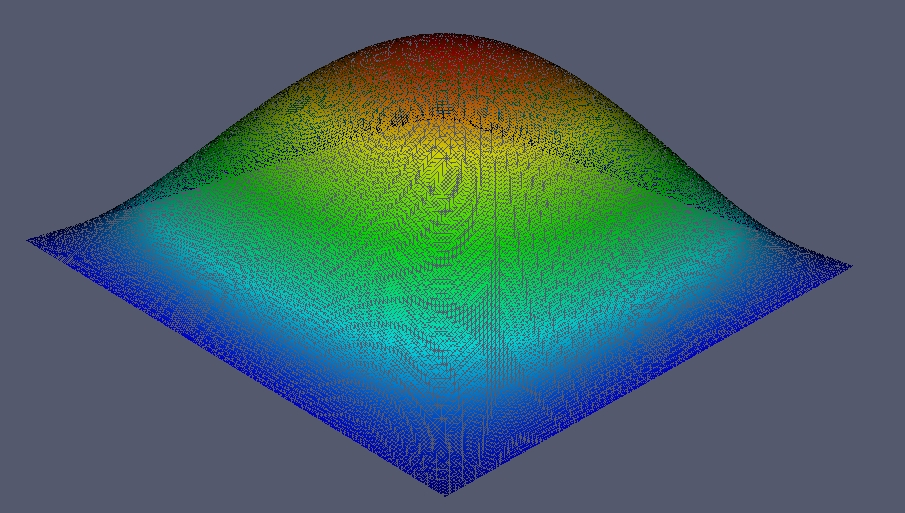
\includegraphics[width=0.8\textwidth]{EPS/fem2d}
\caption{Solution in 2D}
\label{Fig:FEM1}
\end{figure}

\begin{figure}
\centering
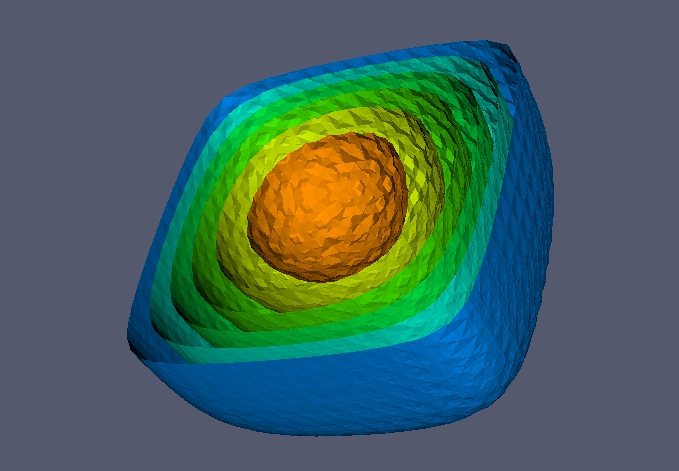
\includegraphics[width=0.8\textwidth]{EPS/fem3d}
\caption{Solution in 3D}
\label{Fig:FEM2}
\end{figure}

\begin{exc}
 Try a 3-dimensional grid! Just change the dimension in line \ref{fem:dim} and the name of the gridfile in line \ref{fem:file} to \lstinline!3dgrid.al! . You can compile the new code without reconfiguring by running
\begin{lstlisting}
make ALBERTA_DIM=3
\end{lstlisting}
\end{exc}

\begin{exc}
 Modify the code in order to make it handle Neumann boundary conditions too!
\end{exc}



\chapter{Adaptivity}

\section{Adaptive integration}

\subsection{Adaptive multigrid integration}

In this section we describe briefly the adaptive multigrid integration
algorithm presented in \cite{Deuflhard93}.

\minisec{Global error estimation}

The global error can be estimated by taking the difference of the numerically
computed value for the integral on a fine and a coarse grid as given in
(\ref{Eq:GlobalError}).

\minisec{Local error estimation}

Let $I_f^p(\omega)$ and $I_f^q(\omega)$ be two integration formulas of
different orders $p>q$ for the evaluation of the integral over some
function $f$ on the element $\omega\subseteq\Omega$. If we assume that
the higher order rule is locally more accurate then
\begin{equation}
\bar{\epsilon}(\omega) = |I_f^p(\omega)-I_f^q(\omega)|
\end{equation}
is an estimator for the local error on the element $\omega$.

\minisec{Refinement strategy}

If the estimated global error is not below a user tolerance the grid
is to be refined in those places where the estimated local error is
``high''. To be more specific, we want to achieve that each element in
the grid contributes about the same local error to the global
error. Suppose we knew the maximum local error on all the new elements
that resulted from refining the current mesh (without actually doing
so). Then it would be a good idea to refine only those elements in the
mesh where the local error is not already below that maximum local
error that will be attained anyway.
In \cite{Deuflhard93} it is shown that the local error after mesh
refinement can be effectively computed without actually doing the
refinement. Consider an element $\omega$ and its father element
$\omega^-$, i.~e.~the refinement of  $\omega^-$ resulted in
$\omega$. Moreover, assume that $\omega^+$ is a (virtual) element that
would result from a refinement of $\omega$. Then it can be shown that
under certain assumptions the quantity
\begin{equation}
\epsilon^+(\omega) = \frac{\bar{\epsilon}(\omega)^2}{\bar{\epsilon}(\omega^-)}
\end{equation}
is an estimate for the local error on $\omega^+$,
i.~e.~$\bar{\epsilon}(\omega^+)$.

Another idea to determine the refinement threshold is to look simply
at the maximum of the local errors on the current mesh and
to refine only those elements where the local error is above a certain
fraction of the maximum local error.

By combining the two approaches we get the threshold value $\kappa$
actually used in the code:
\begin{equation}
\kappa = \min\left(\max\limits_{\omega} \epsilon^+(\omega), \frac12
  \max\limits_{\omega} \bar{\epsilon}(\omega) \right).
\end{equation}

\minisec{Algorithm}

The complete multigrid integration algorithm then reads as follows:
\begin{itemize}
\item Choose an initial grid.
\item Repeat the following steps
\begin{itemize}
\item Compute the value $I$ for the integral on the current grid.
\item Compute the estimate $E$ for the global error.
\item If $E<\text{tol}\cdot I$ we are done.
\item Compute the threshold $\kappa$ as defined above.
\item Refine all elements $\omega$ where $\bar{\epsilon}(\omega)\geq\kappa$.
\end{itemize}
\end{itemize}

\subsection{Implementation of the algorithm}

The algorithm above is realized in the following code.

\begin{lst}[File dune-grid-howto/adaptiveintegration.cc] \mbox{}
\nopagebreak
\lstinputlisting[basicstyle=\ttfamily\scriptsize,numbers=left,
numberstyle=\tiny, numbersep=5pt]{../adaptiveintegration.cc}
\end{lst}

The work is done in the function \lstinline!adaptiveintegration!.
Lines \ref{aic:int0}-\ref{aic:int1} compute the value of the integral
on the current mesh. After printing the result the decision whether
to continue or not is done in line \ref{aic:finish}. The extrapolation
strategy relies on the fact that every element has a father. To ensure
this, the grid is at least once refined globally in the first step
(line \ref{aic:gr}). Now the refinement threshold $\kappa$ can be
computed in lines \ref{aic:kappa0}-\ref{aic:kappa1}. Finally the last
loop in lines \ref{aic:mark0}-\ref{aic:mark1} marks elements for
refinement and lines \ref{aic:ref0}-\ref{aic:ref1} actually do the
refinement. The reason for dividing refinement into three functions
\lstinline!preAdapt()!, \lstinline!adapt()! and
\lstinline!postAdapt()! will be explained with the next example. Note
the flexibility of this algorithm: It runs in any space dimension on
any kind of grid and different integration orders can easily be
incorporated. And that with just about 100 lines of code including
comments.

\begin{figure}
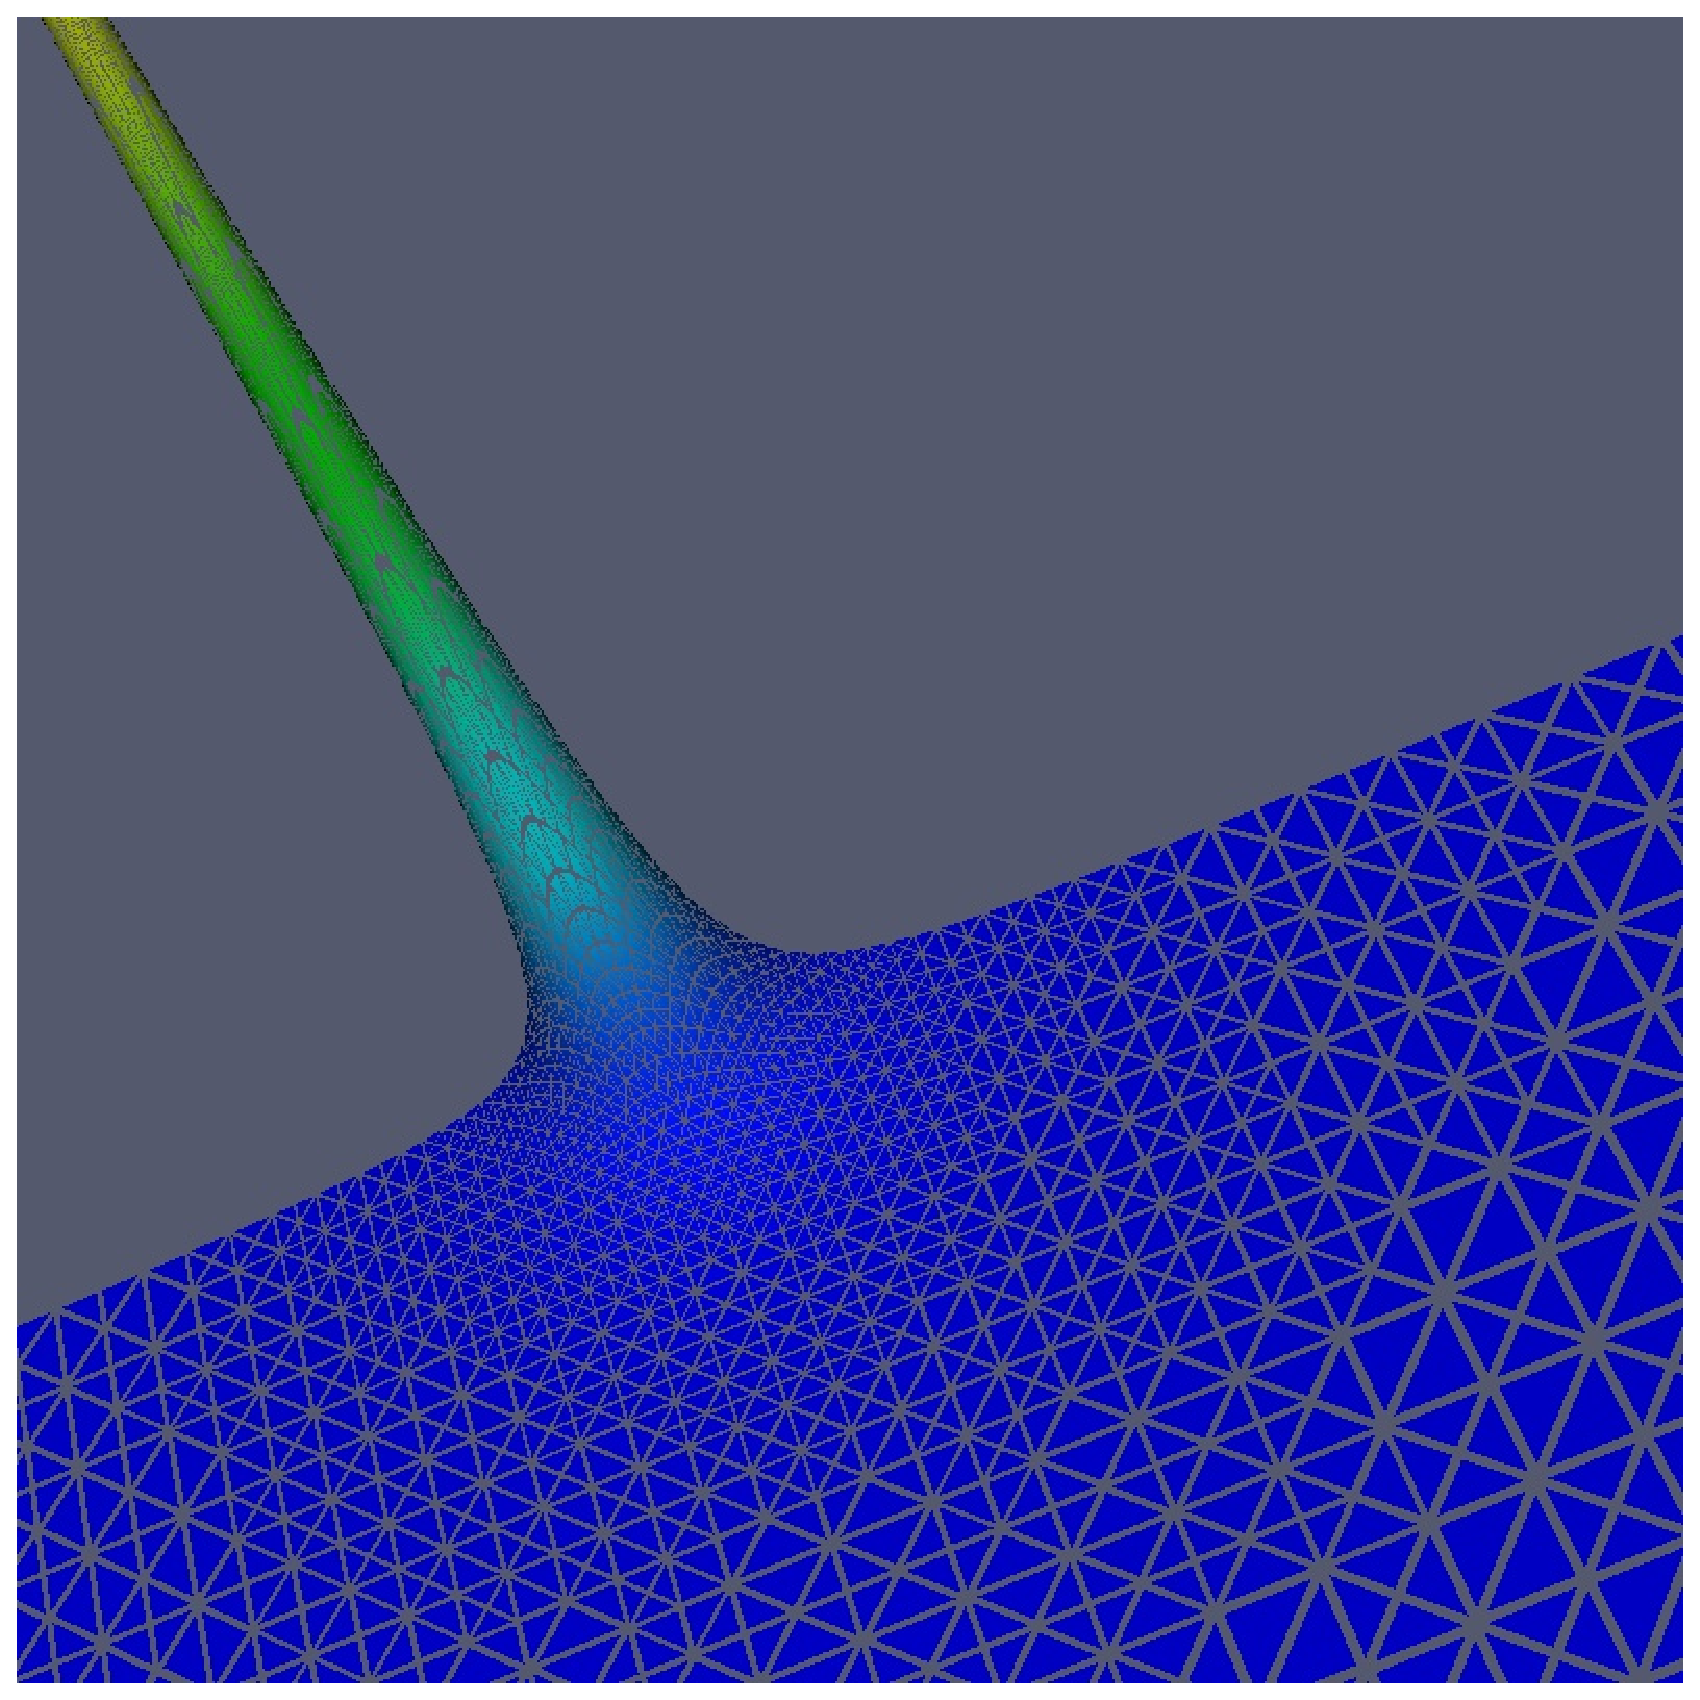
\includegraphics[width=0.48\textwidth]{EPS/adaptiveintegration_alberta2d}\hfill
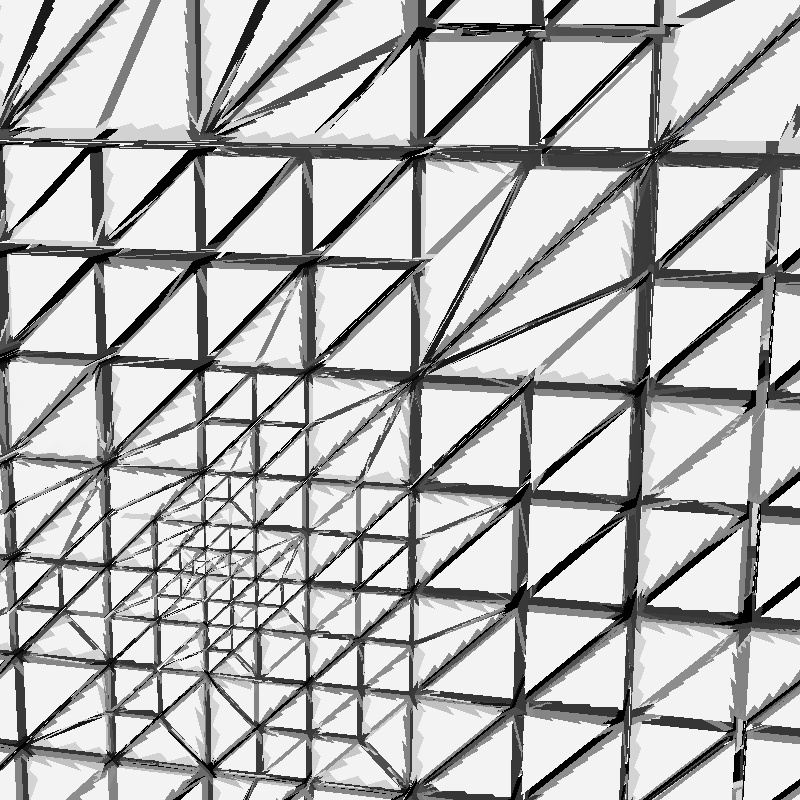
\includegraphics[width=0.48\textwidth]{EPS/adaptiveintegration_ug3d}
\caption{Two and three-dimensional grids generated by the adaptive
  integration algorithm applied to the needle pulse. Left grid is
  generated using Alberta, right grid is generated using UG.}
\label{Fig:AdaptiveIntegration}
\end{figure}

Figure \ref{Fig:AdaptiveIntegration} shows two grids generated by the
adaptive integration algorithm.

\begin{warn} The quadrature rules for prisms and pyramids are
  currently only implemented for order two. Therefore adaptive
  calculations with UGGrid and hexahedral elements do not work.
\end{warn}



\section{Adaptive cell centered finite volumes}

In this section we extend the example of Section
\ref{Sec:CellCenteredFV} by adaptive mesh refinement. This requires
two things: (i) a method to select cells for refinement or coarsening
(derefinement) and (ii) the transfer of a solution on a given grid to
the adapted grid. The finite volume algorithm itself has already been
implemented for adaptively refined grids in Section
\ref{Sec:CellCenteredFV}.

For the adaptive refinement and coarsening we use a very simple
heuristic strategy that works as follows:
\begin{itemize}
\item Compute global maximum and minimum of element concentrations:
  $$\overline{C}=\max_i C_i,  \ \ \ \underline{C}=\min_i C_i.$$
\item As the local indicator in cell $\omega_i$ we define $$\eta_i =
  \max_{\gamma_{ij}} |C_i-C_j|.$$ Here $\gamma_{ij}$ denotes
  intersections with other elements in the leaf grid.
\item If for $\omega_i$ we have
  $\eta_i>\overline{\text{tol}}\cdot (\overline{C}-\underline{C})$
  and $\omega_i$ has not been refined more than $\overline{M}$ times
  then mark $\omega_i$ and all its neighbors for refinement.
\item Mark all elements $\omega_i$ for coarsening where
  $\eta_i<\underline{\text{tol}}\cdot (\overline{C}-\underline{C})$
  and $\omega_i$ has been refined at least $\underline{M}$ times.
\end{itemize}

This strategy refines an element if the local gradient is ``large''
and it coarsens elements (which means it removes a previous
refinement) if the local gradient is ``small''. In addition any
element is refined at least refined $\underline{M}$ times and at most
$\overline{M}$ times.

After mesh modification the solution from the previous grid must be
transfered to the new mesh. Thereby the following situations do occur
for an element:
\begin{itemize}
\item The element is a leaf element in the new mesh and was a leaf
  element in the old mesh: keep the value.
\item The element is a leaf element in the new mesh and existed in the
  old mesh as a non-leaf element: Compute the cell value as an average
  of the son elements in the old mesh.
\item The element is a leaf element in the new mesh and is obtained
  through refining some element in the old mesh: Copy the value
  from the element in the old mesh to the new mesh.
\end{itemize}

The complete mesh adaptation is done by the function
\lstinline!finitevolumeadapt! in the following listing:

\begin{lst}[File dune-grid-howto/finitevolumeadapt.hh] \mbox{}
\nopagebreak
\lstinputlisting[basicstyle=\ttfamily\scriptsize,numbers=left,
numberstyle=\tiny, numbersep=5pt]{../finitevolumeadapt.hh}
\end{lst}

The loop in lines \ref{fah:loop0}-\ref{fah:loop1} computes the
indicator values $\eta_i$ as well as the global minimum and maximum
$\overline{C},\underline{C}$. Then the next loop in lines
\ref{fah:loop2}-\ref{fah:loop3} marks the elements for refinement.
Lines \ref{fah:loop4}-\ref{fah:loop5} construct a map that stores for
each element in the mesh (on all levels) the average of the element
values in the leaf elements of the subtree of the given element. This
is accomplished by descending from the fine grid levels to the coarse
grid levels and thereby adding the value in an element to the father
element. The key into the map is the global id of an element. Thus the
value is accessible also after mesh modification.

Now the grid can really be modified in line \ref{fah:adapt} by calling the
\lstinline!adapt()! method on the grid object. The mapper is updated
to reflect the changes in the grid in line \ref{fah:update} and the
concentration vector is resized to the new size in line
\ref{fah:resize}. Then the values have to be interpolated to the new
elements in the mesh using the map and finally to be transferred to
the resized concentration vector. This is done in the loop in lines
\ref{fah:loop6}-\ref{fah:loop7}.

Here is the new main program with an adapted \lstinline!timeloop!:

\begin{lst}[File dune-grid-howto/adativefinitevolume.cc] \mbox{}
\nopagebreak
\lstinputlisting[basicstyle=\ttfamily\scriptsize,numbers=left,
numberstyle=\tiny, numbersep=5pt]{../adaptivefinitevolume.cc}
\end{lst}

The program works analogously to the non adaptive \lstinline!finitevolume!\
version from the previous chapter. The only differences are inside the
\lstinline!timeloop!\ function. During the initialization of the concentration
vector in line \ref{afv:in} and after each time step in line \ref{afv:ad} the
function \lstinline!finitevolumeadapt! is called in order to refine the grid.
The initial adaptation is repeated $\overline{M}$ times.  Note that adaptation
after each time steps is deactivated during the compiler phase for unstructured
grids with help of the \lstinline!Capabilities!\ class. This is because
structured grids do not allow a conforming refinement and are therefore
unusable for adaptive schemes. In fact, the \lstinline!adapt! method on a grid
of \lstinline!YaspGrid! e.\,g.~ results in a {\em global} grid refinement.

\begin{exc}
  Compile the program with the gridtype set to \lstinline!ALUGRID_SIMPLEX!
  and \lstinline!ALUGRID_CONFORM! and compare the results visually.
\end{exc}

\chapter{Parallelism}

\section{\texorpdfstring{\Dune{}}{DUNE} Data Decomposition Model}

The parallelization concept in \Dune{} follows the Single Program
Multiple Data (SPMD) data parallel programming paradigm. In this
programming model each process executes the same code but on different
data. The parallel program is parametrized
by the rank of the individual process in the set and the number of
processes $P$
involved. The processes communicate by exchanging messages, but you
will rarely have the need to bother with sending messages.

A parallel \Dune{} grid, such as YaspGrid, is a collective object which
means that all processes participating in the computations on the grid
instantiate the grid object at the same time (collectively). Each
process stores a subset of all the entities that the same program running on a
single process would have. An entity may be stored in more
than one process, in principle it may be even stored in all
processes. An entity
stored in more than one process is called a distributed entity. \Dune{}
allows quite general data decompositions but not arbitrary data
decompositions. Each entity in a process has a partition type
value assigned to it. There are five different possible partition type
values:
\begin{center}
\textit{interior}, \textit{border}, \textit{overlap},
  \textit{front} and \textit{ghost}.
\end{center}

Entities of codimension 0 are restricted to the three partition types
\textit{interior}, \textit{overlap} and \textit{ghost}. Entities of
codimension greater than 0 may take all partition type values.
The codimension 0 entities with partition type \textit{interior} form a
non-overlapping decomposition of the entity set, i.e.~for each
entity of codimension 0 there is exactly one process where this entity
has partition type \textit{interior}.
Moreover, the codimension 0 leaf entities in process number $i$ form a
subdomain $\Omega_i\subseteq\Omega$ and all the $\Omega_i$, $0\leq i <
P$, form a nonoverlapping decomposition of the computational domain
$\Omega$. The leaf entities of codimension 0 in a process $i$ with
partition types \textit{interior} or \textit{overlap} together form a
subdomain $\hat{\Omega}_i\subseteq\Omega$.

Now the partition types of the entities in process $i$
with codimension greater 0 can
be determined according to the following table:
\begin{center}
\begin{tabular}{cc}
\hline
\hline
Entity located in & Partition Type value\\
\hline
$B_i=\overline{\partial\Omega_i\setminus\partial\Omega}$ &
\textit{border}\\
$\overline{\Omega_i}\setminus B_i$ & \textit{interior}\\
$F_i =
\overline{\partial\hat{\Omega}_i\setminus\partial\Omega}\setminus B_i$
& \textit{front}\\
$\overline{\hat{\Omega}_i}\setminus(B_i\cup F_i)$ & \textit{overlap}\\
Rest & \textit{ghost}\\
\hline
\hline
\end{tabular}
\end{center}

\begin{figure}
\centering
\begin{overpic}[width=\textwidth]{EPS/partitionsingle}
 \put(12,62){$c=0$}
 \put(45,62){$c=1$}
 \put(80,62){$c=2$}

 \put(12,31){$c=0$}
 \put(45,31){$c=1$}
 \put(80,31){$c=2$}

 \put(12,1){$c=0$}
 \put(45,1){$c=1$}
 \put(80,1){$c=2$}
\end{overpic}

\caption{Color coded illustration of different data decompositions:
  interior (red), border (blue), overlap (green), front (magenta) and
  ghost (yellow), gray encodes entities not stored by the
  process. First row shows case with interior, overlap and ghost
  entities, second row shows a case with interior and overlap without
  ghost and the last row shows a case with interior and ghost only.}
\label{Fig:PartitionSingle}
\end{figure}

The assignment of partition types is illustrated for three different
examples in Figure \ref{Fig:PartitionSingle}. Each example shows a
two-dimensional structured grid with $6\times 4$ elements (in
gray). The entities stored in some process $i$ are shown in color,
where color indicates the partition type as explained in the
caption. The first row shows an example where process $i$ has
codimension 0 entities of all three partition types \textit{interior},
\textit{overlap} and \textit{ghost} (leftmost picture in first
row). The corresponding assignment of partition types to entities of
codimension 1 and 2 is then shown in the middle and right most
picture. A grid implementation can choose to omit the partition type
\textit{overlap}  or \textit{ghost} or both, but not
\textit{interior}. The middle row shows an example where an
\textit{interior} partition is extended by an \textit{overlap} and no
\textit{ghost} elements are present. This is the model used in
YaspGrid. The last row shows an example where the \textit{interior} partition
is extended by one row of  \textit{ghost} cells. This is the model
used in UGGrid and ALUGrid.


\section{Communication Interfaces}

This section explains how the exchange of data between the partitions
in different processes is organized in a flexible and portable way.

The abstract situation is that data has to be sent from a copy of a
distributed entity in a process to one or more copies of the same
entity in other processes. Usually data has to be sent not only for
one entity but for many entities at a time, thus it is more efficient
pack all data that goes to the same destination process into a single
message. All entities for which data has to be sent or received form a
so-called \textit{communication interface}. As an example let us define the set
$X_{i,j}^c$ as the set of all entities of codimension $c$ in process $i$
  with partition type \textit{interior} or \textit{border} that have
a copy in process $j$ with any partition type. Then in the
communication step process $i$ will send one message to any other
process $j$ when $X_{i,j}^c\neq\emptyset$. The message contains some data for
every entity in  $X_{i,j}^c$. Since all processes participate in the
communication step, process $i$ will receive data from a process $j$
whenever $X_{j,i}^c\neq\emptyset$. This data corresponds to entities
in process $i$ that have a copy in $X_{j,i}^c$.

A \Dune{} grid offers a selection of predefined interfaces. The example
above would use the parameter \lstinline!InteriorBorder_All_Interface!
in the communication function. After the
selection of the interface it remains to specify the data to be sent
per entity and how the data should be processed at the receiving
end. Since the data is in user space the user has to write a small
class that encapsulates the processing of the data at the sending and
receiving end. The following listing shows an example for a so-called
data handle:


\begin{lst}[File dune-grid-howto/parfvdatahandle.hh] \mbox{}
\nopagebreak
\lstinputlisting[basicstyle=\ttfamily\scriptsize,numbers=left,
numberstyle=\tiny, numbersep=5pt]{../parfvdatahandle.hh}
\end{lst}

Every instance of the \lstinline!VectorExchange! class template
conforms to the data handle concept. It defines a type
\lstinline!DataType! which is the type of objects that are exchanged
in the messages between the processes. The method \lstinline!contains!
should return true for all codimensions that participate in the data
exchange. Method \lstinline!fixedsize! should return true when, for
the given codimension, the same number of data items per entity is
sent. If \lstinline!fixedsize! returns false the method
\lstinline!size! is called for each entity in order to ask
for the number of items of type \lstinline!DataType! that are to be
sent for the given entity. Note that this information has only to be
given at the sender side. Then the method \lstinline!gather! is called
for each entity in a communication interface on the sender side in
order to pack the data for this entity into the message buffer. The
message buffer itself is realized as an output stream that accepts data
of type \lstinline!DataType!. After exchanging the data via message
passing the \lstinline!scatter! method is called for each entity at
the receiving end. Here the data is read from the message buffer and
stored in the user's data structures. The message buffer is realized
as an input stream delivering items of type \lstinline!DataType!. In
the \lstinline!scatter! method it is up to the user how the data is to
be processed, e.\,g.~one can simply overwrite (as is done here), add or
compute a maximum.

\section{Parallel finite volume scheme}

In this section we parallelize the (nonadaptive!) cell centered finite volume
scheme. Essentially only the \lstinline!evolve! method has to be
parallelized. The following listing shows the parallel version of this
method. Compare this with listing \ref{List:evolve} on page \pageref{List:evolve}.

\begin{lst}[File dune-grid-howto/parevolve.hh] \mbox{}
\nopagebreak
\lstinputlisting[basicstyle=\ttfamily\scriptsize,numbers=left,
numberstyle=\tiny, numbersep=5pt]{../parevolve.hh}
\end{lst}

The first difference to the sequential version is in line
\ref{peh:assert} where it is checked that the grid provides an overlap
of at least one element. The overlap may be either of partition type
\textit{overlap} or \textit{ghost}. The finite volume scheme itself
only computes the updates for the elements with partition type
\textit{interior}.

In order to iterate over entities with a specific partiton type the
leaf and level iterators can be parametrized by an additional argument
\lstinline!PartitionIteratorType! as shown in line \ref{peh:pit}. If
the argument \lstinline!All_Partition! is given then all entities are
processed, regardless of their partition type. This is also the
default behavior of the level and leaf iterators. If the partition
iterator type is specified explicitely in an iterator the same
argument has also to be specified in the begin and end methods on the
grid as shown in lines \ref{peh:end}-\ref{peh:begin}.

The next change is in line \ref{peh:inter} where the computation of
the optimum stable time step is restricted to elements of partition
type \textit{interior} because only those elements have all neighboring
elements locally available. Next, the global minimum of the time steps
sizes determined in each process is taken in line \ref{peh:min}. For
collective communication each grid returns a collective communication
object with its \lstinline!comm()! method which allows to compute
global minima and maxima, sums, broadcasts and other functions.

Finally the updates computed on the \textit{interior} cells in each
process have to be sent to all copies of the respective entities in
the other processes. This is done in lines
\ref{peh:dist0}-\ref{peh:dist1} using the data handle described above.
The \lstinline!communicate! method on the grid uses the data handle to
assemble the message buffers, exchanges the data and writes the data
into the user's data structures.

Finally, we need a new main program, which is in the following listing:

\begin{lst}[File dune-grid-howto/parfinitevolume.cc] \mbox{}
\nopagebreak
\lstinputlisting[basicstyle=\ttfamily\scriptsize,numbers=left,
numberstyle=\tiny, numbersep=5pt]{../parfinitevolume.cc}
\end{lst}

A difference to the sequential program can be found in line
\ref{pfc:rank0} where the printing of the data of the current time
step is restricted to the process with rank 0.
\lstinline!YaspGrid! does not support dynamical load balancing and therefore
needs to start with a sufficiently fine grid that allows a reasonable partition
where each processes gets a non-empty part of grid. This is why we do not use
DGF Files in the parallel example and initialize the grid by the UnitCube class
instead. For \lstinline!YaspGrid! this allows an easy selection of the grid's
initial coarseness through the second template argument of the
\lstinline!UnitCube!. This argument should be chosen sufficiently high, because
after each global refinement step the overlap region grows and therefore the
communicaton overhead increases.

If you want to use a grid with support for dynamical load balancing, uncomment
one of the possible definitions for such a grid in the code and define the
macro \lstinline!LOAD_BALANCING!. In this case in line \ref{pfv:lb} the method
\lstinline!loadBalance!\ is called on the grid.
This method re-partitions the grid in a way such that on every partition there
is an equal amount of grid elements.

% \chapter{Input and Output}

% \section{Visualization with Grape}



% \section{Visualization with VTK}

% \section{Dune portable grid format}

% Dune provides a unified macro grid format called the
% \textbf{D}une \textbf{G}rid \textbf{F}ormat, short the \textbf{DGF}.
% This enables the user to use all types of grids with one and the same
% macro grid file. For the documentation of the DGF and the usage of the parser we refer to

% \href{http://www.dune-project.org/doc/doxygen/dune-grid-html/group\_\_DuneGridFormatParser.html}%
% {{\small\texttt{http://www.dune-project.org/doc/doxygen/dune-grid-html/group\_\_DuneGridFormatParser.html}}}

% in the dune-grid documentation.

% \section{Amiramesh output}


% \chapter{Iterative Solver Template Library}

% \begin{lst}[File dune-grid-howto/groundwater.cc] \mbox{}
% \nopagebreak
% \lstinputlisting[basicstyle=\ttfamily\scriptsize,numbers=left,
% numberstyle=\tiny, numbersep=5pt]{../groundwater.cc}
% \end{lst}

% \begin{lst}[File dune-grid-howto/groundwaterproblem.hh] \mbox{}
% \nopagebreak
% \lstinputlisting[basicstyle=\ttfamily\scriptsize,numbers=left,
% numberstyle=\tiny, numbersep=5pt]{../groundwaterproblem.hh}
% \end{lst}

% \begin{lst}[File dune-grid-howto/groundwateradapt.hh] \mbox{}
% \nopagebreak
% \lstinputlisting[basicstyle=\ttfamily\scriptsize,numbers=left,
% numberstyle=\tiny, numbersep=5pt]{../groundwateradapt.hh}
% \end{lst}


% \chapter{Outlook}


\begin{figure}
\centering
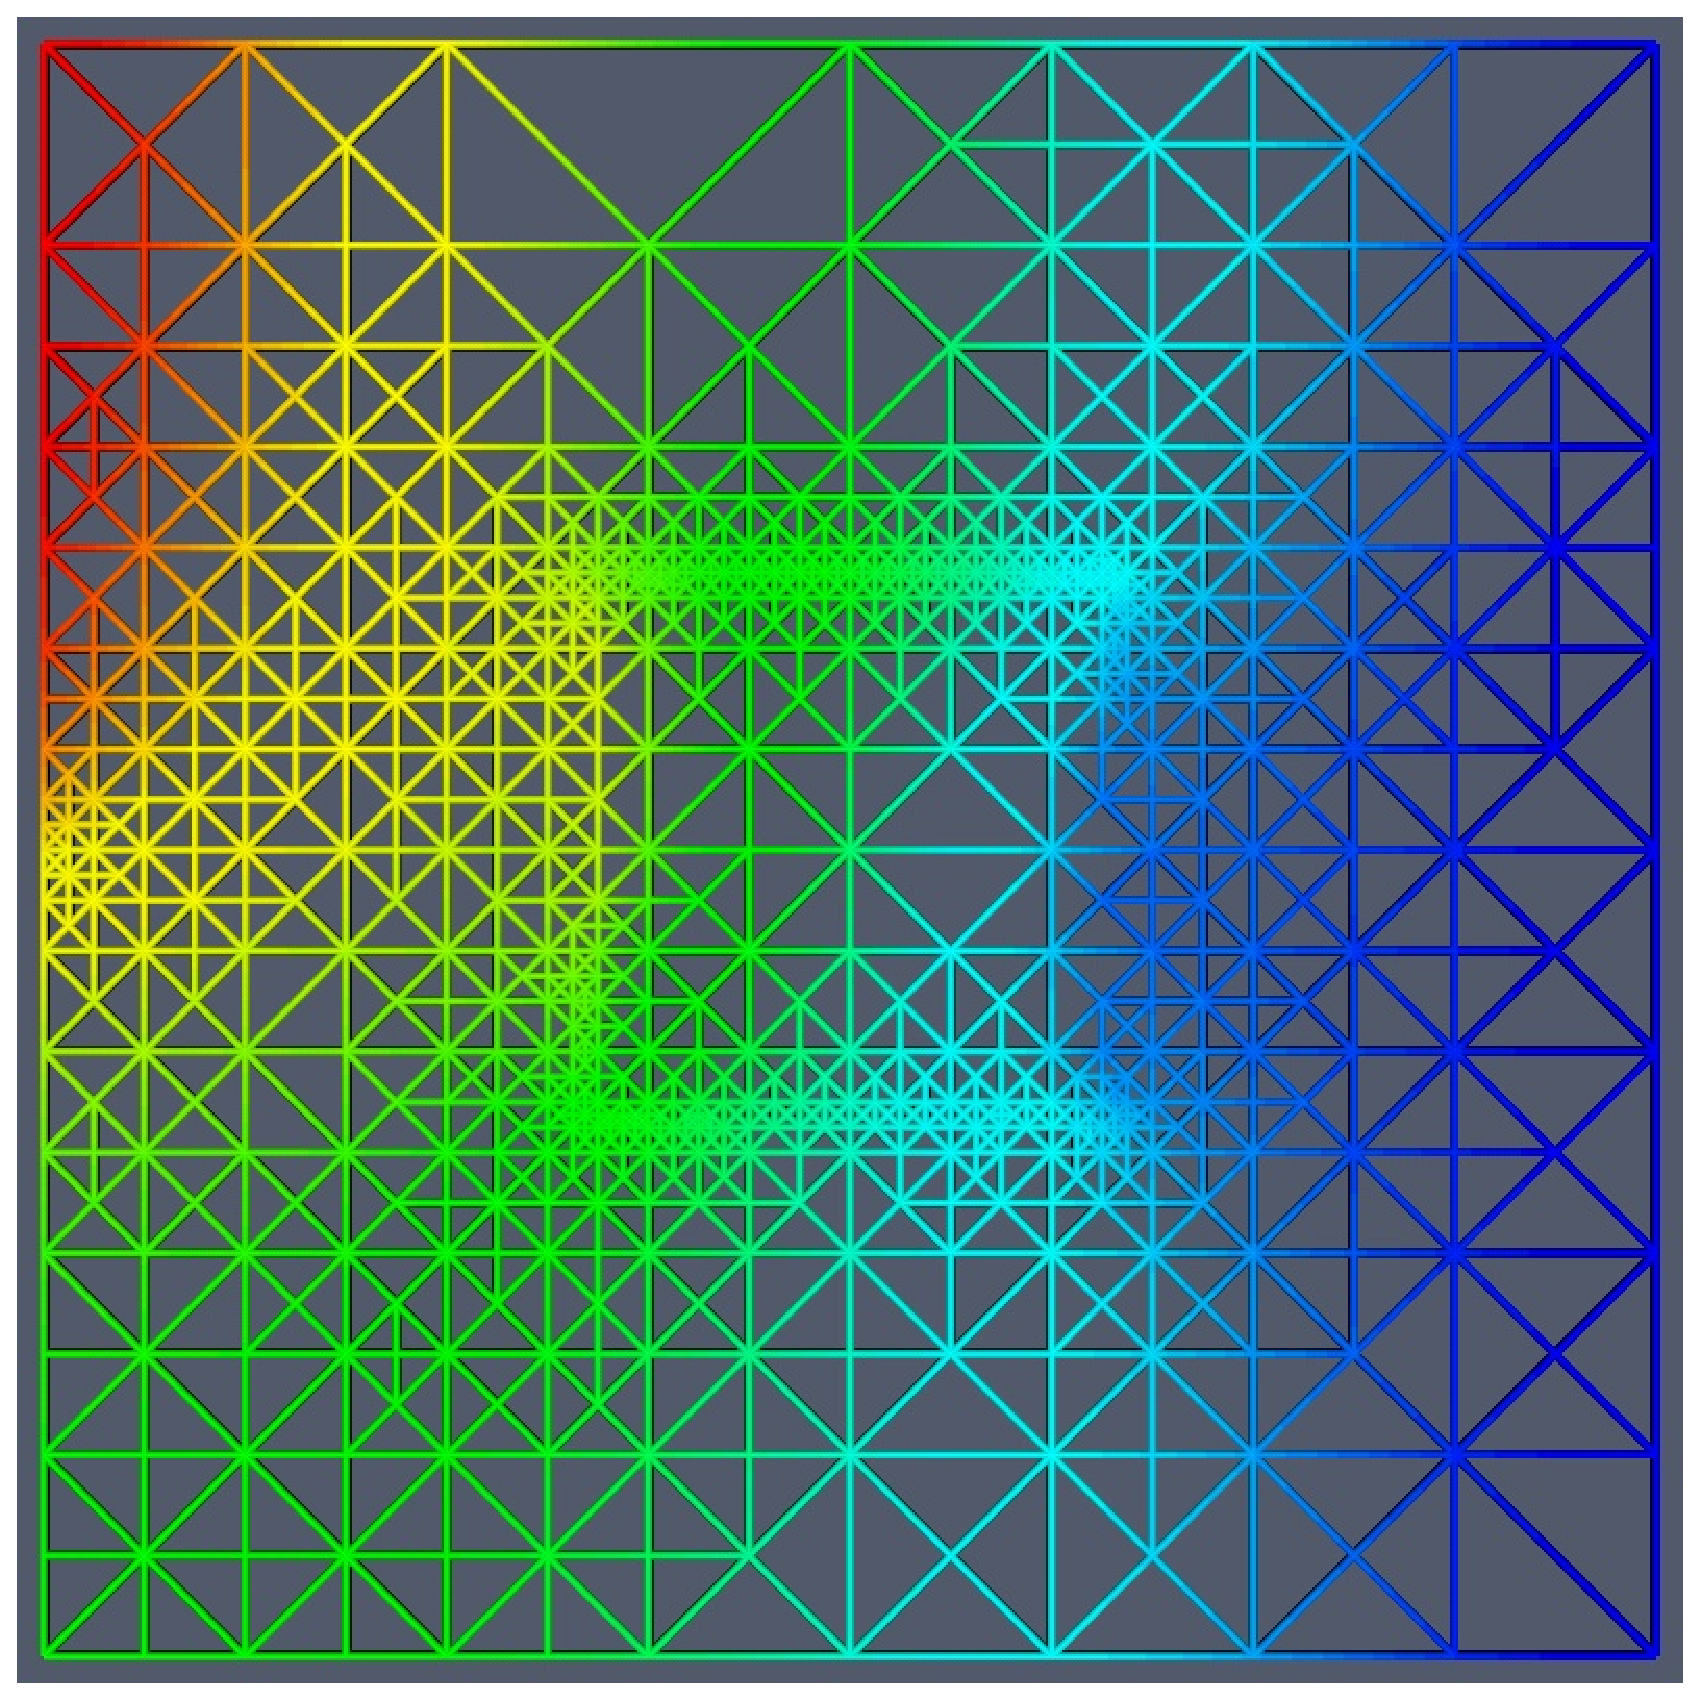
\includegraphics[width=0.32\textwidth]{EPS/alberta2d}\
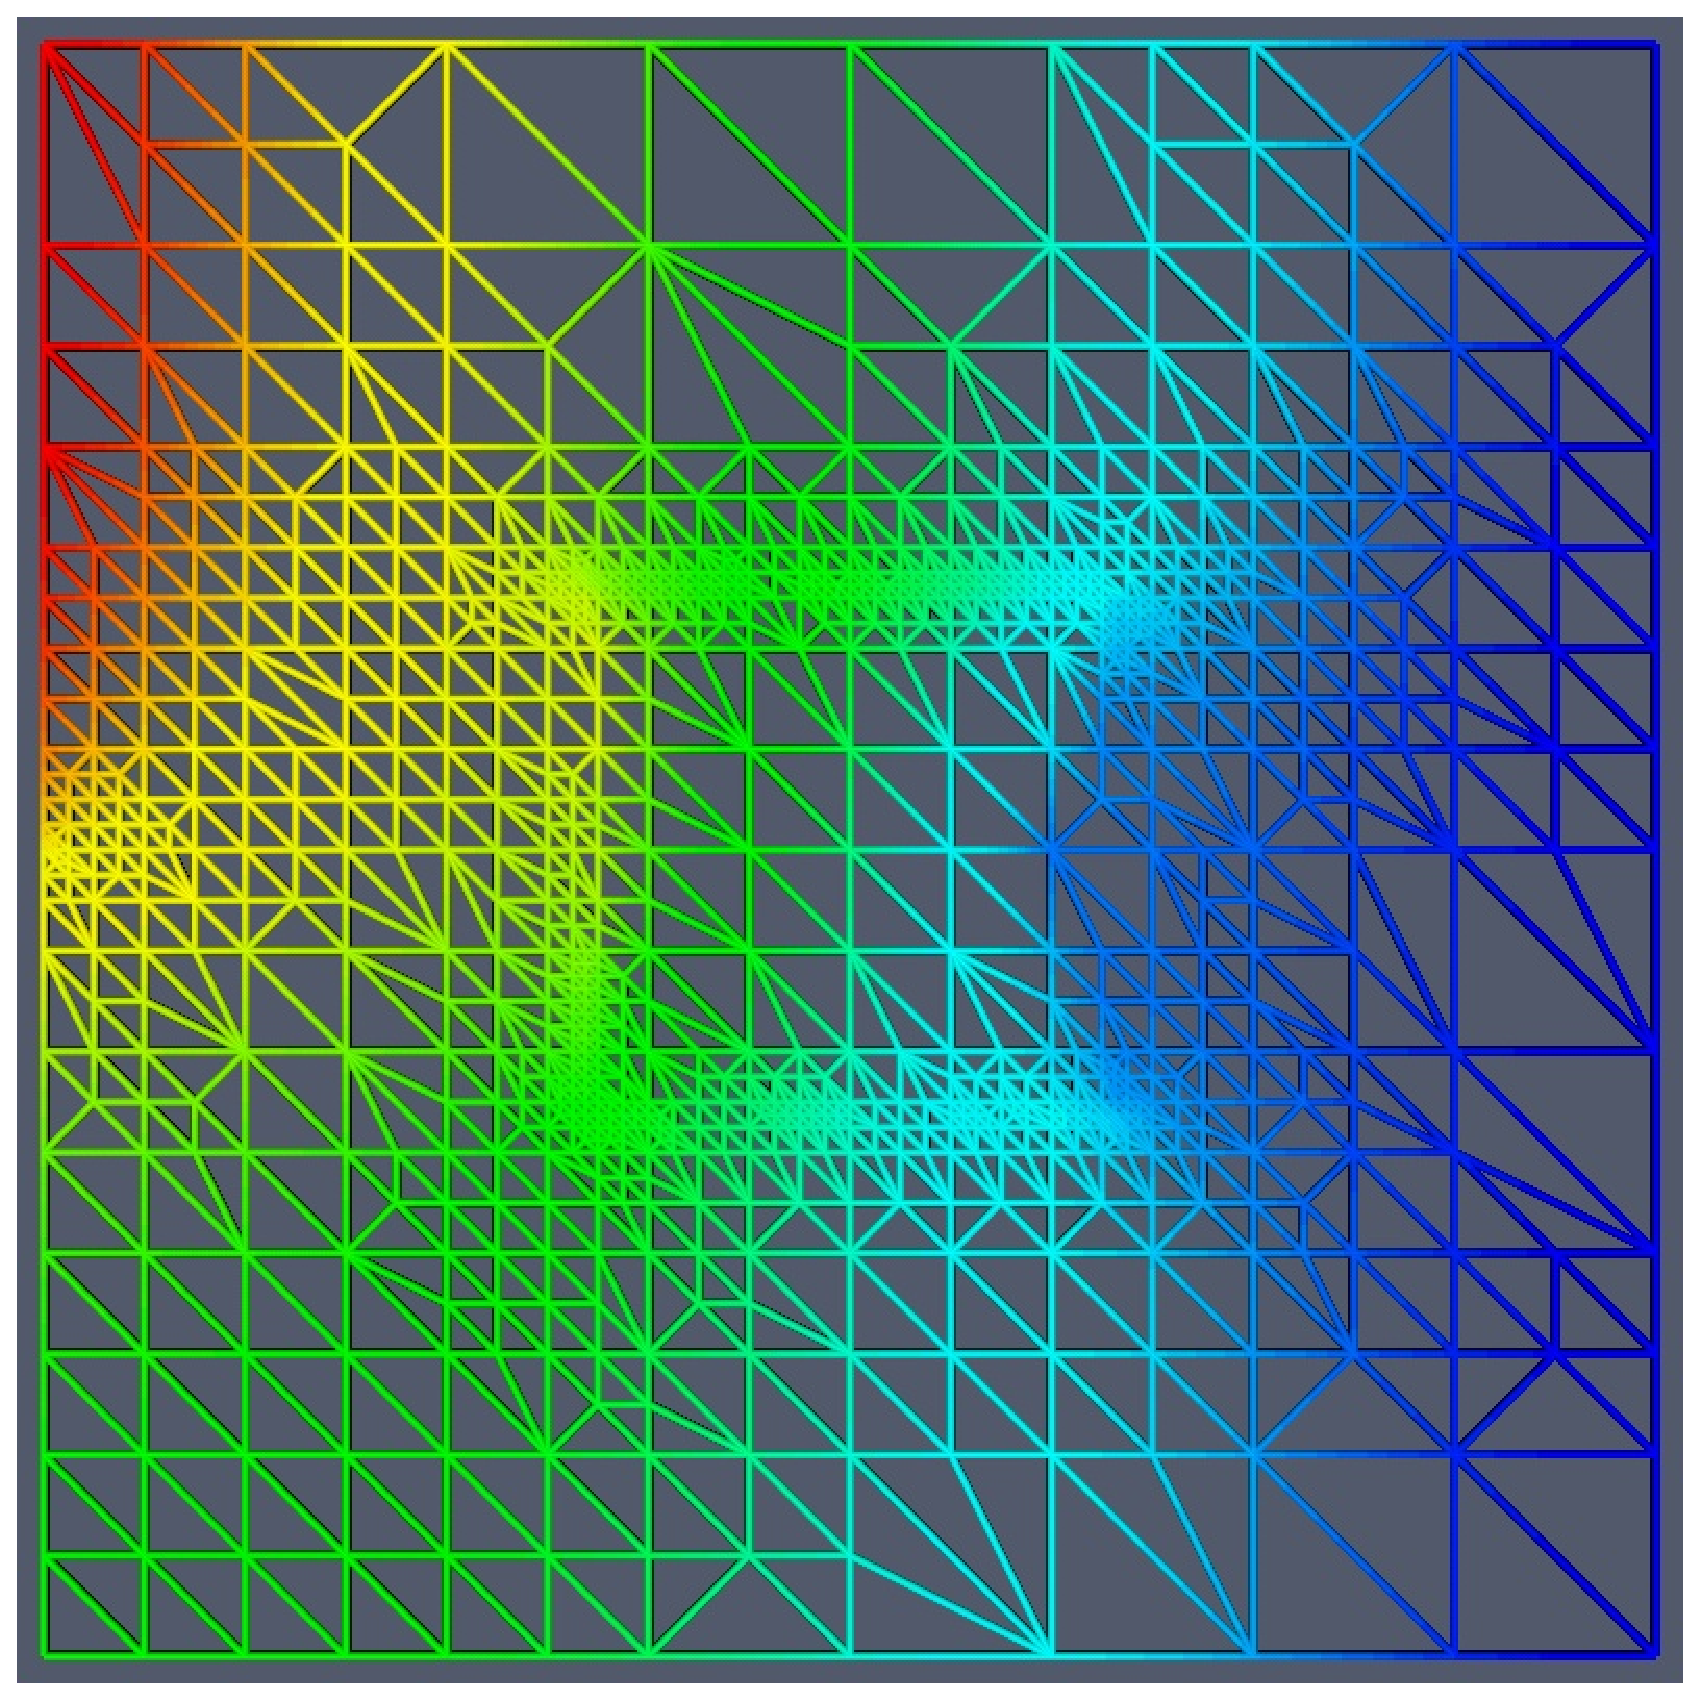
\includegraphics[width=0.32\textwidth]{EPS/ugsimplex2d}\
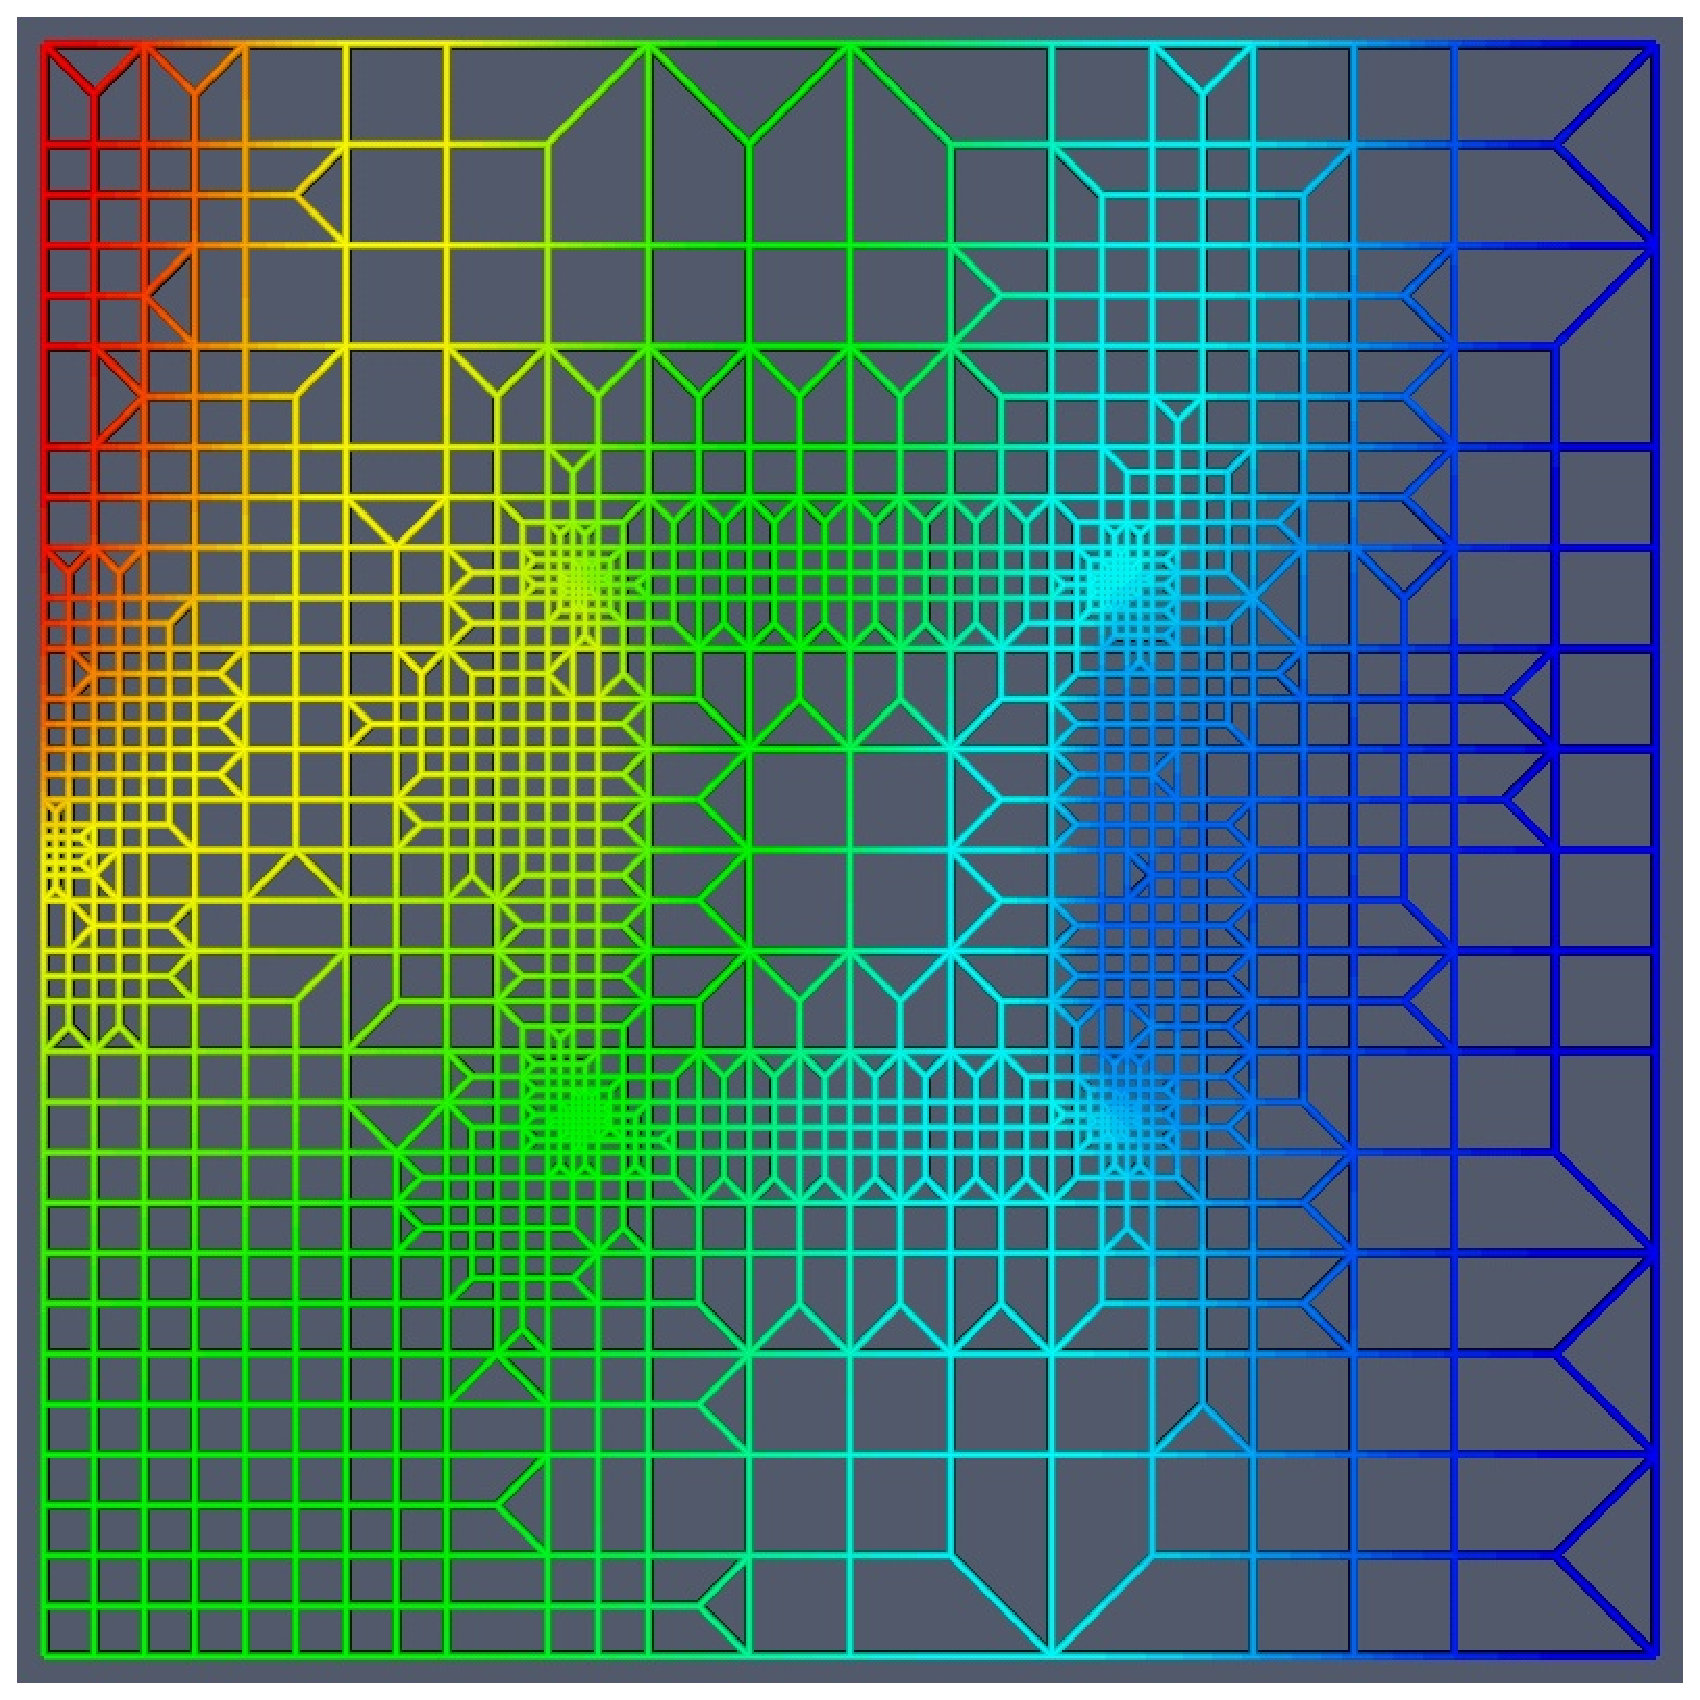
\includegraphics[width=0.32\textwidth]{EPS/ugcube2d}

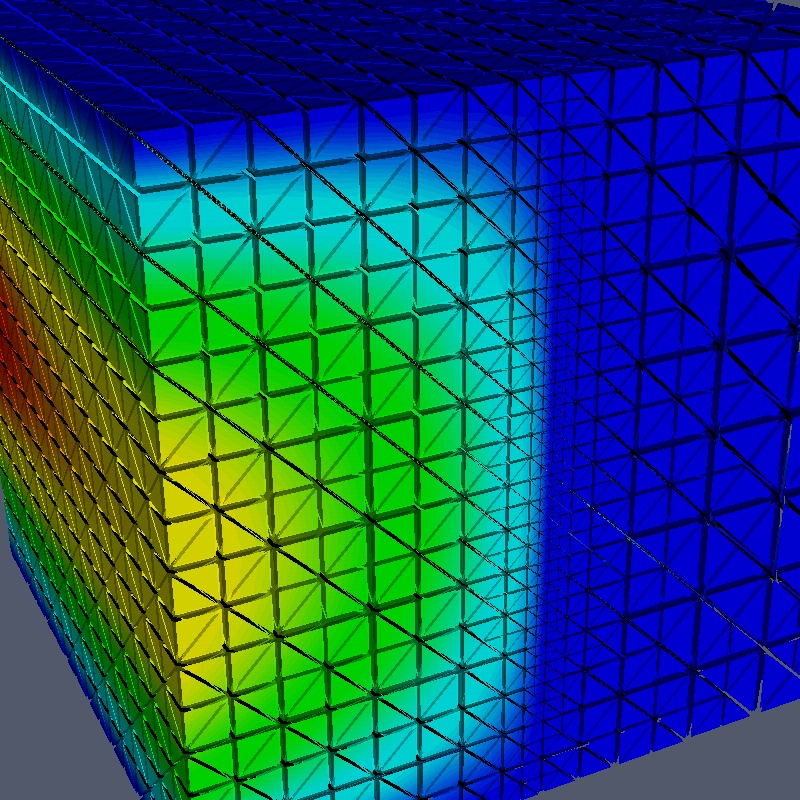
\includegraphics[width=0.32\textwidth]{EPS/alberta3d}\
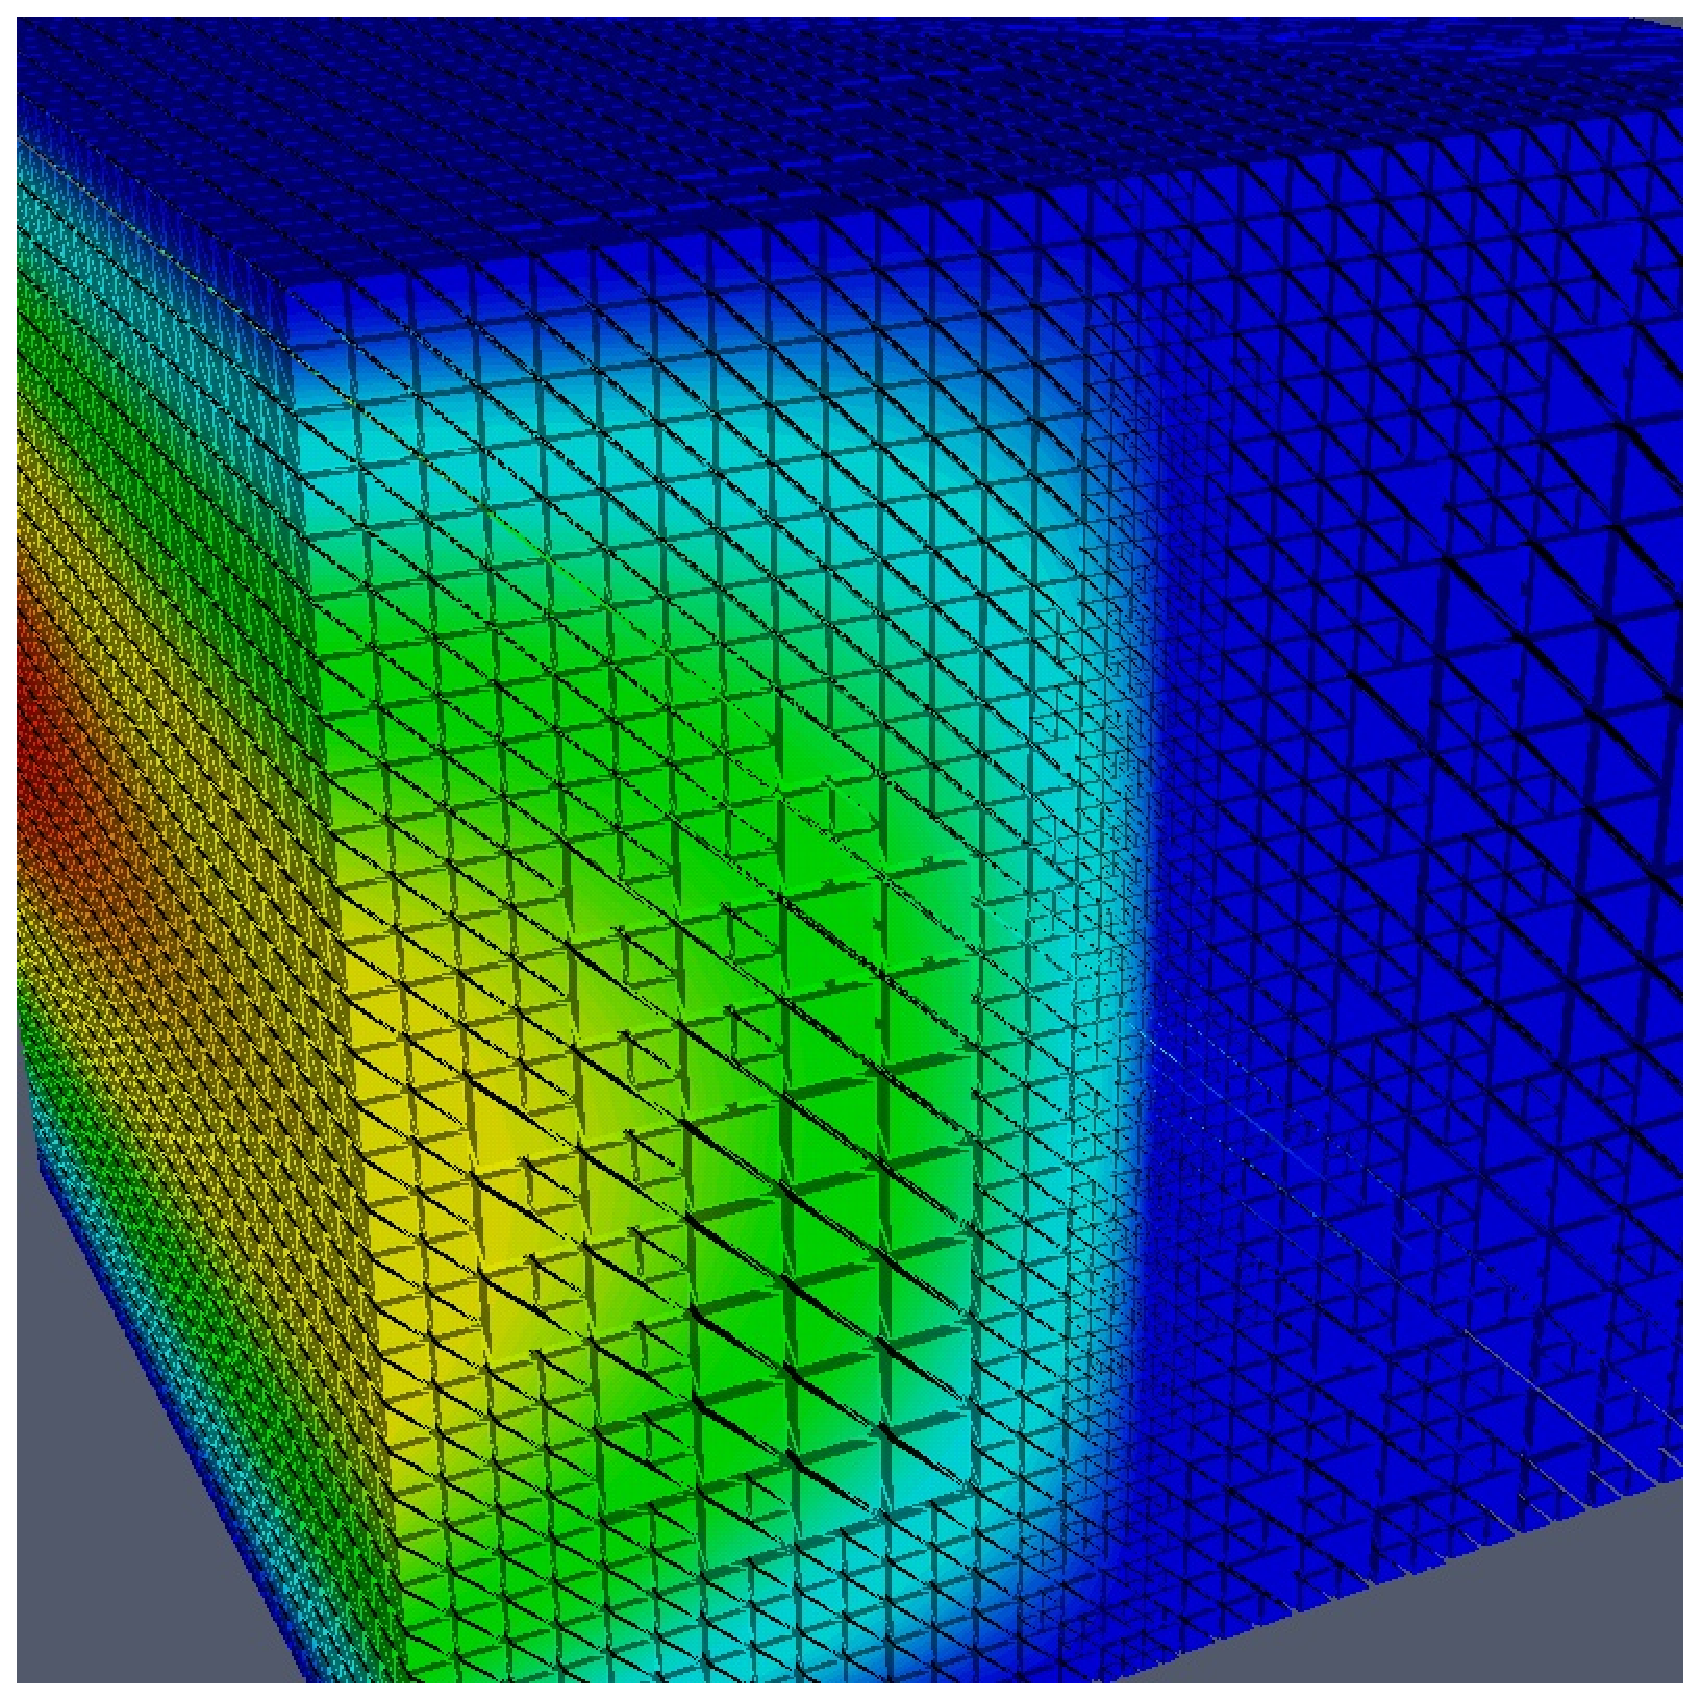
\includegraphics[width=0.32\textwidth]{EPS/alusimplex3d}\
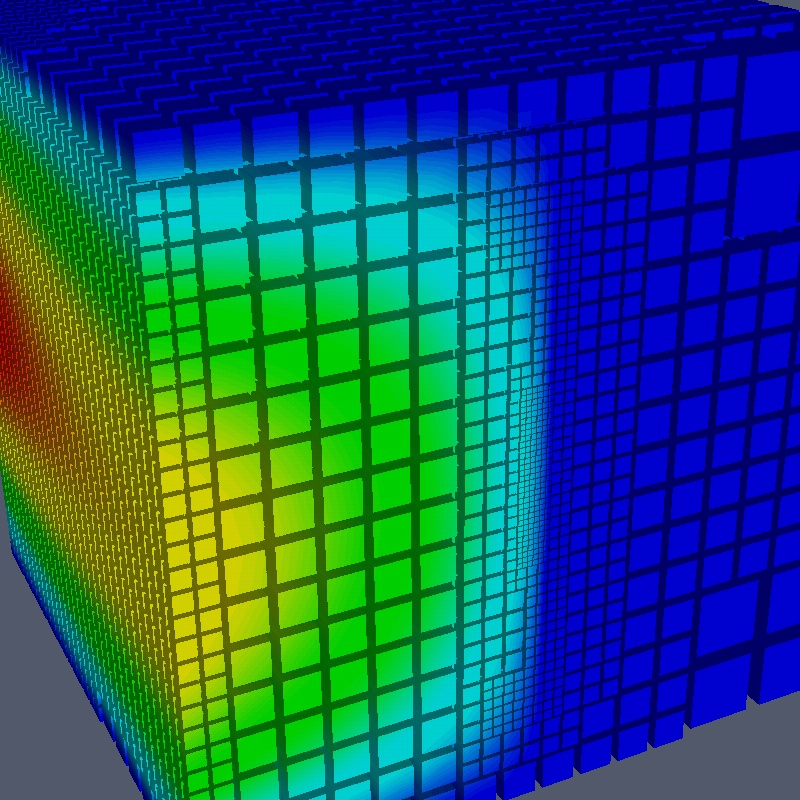
\includegraphics[width=0.32\textwidth]{EPS/alucube3d}


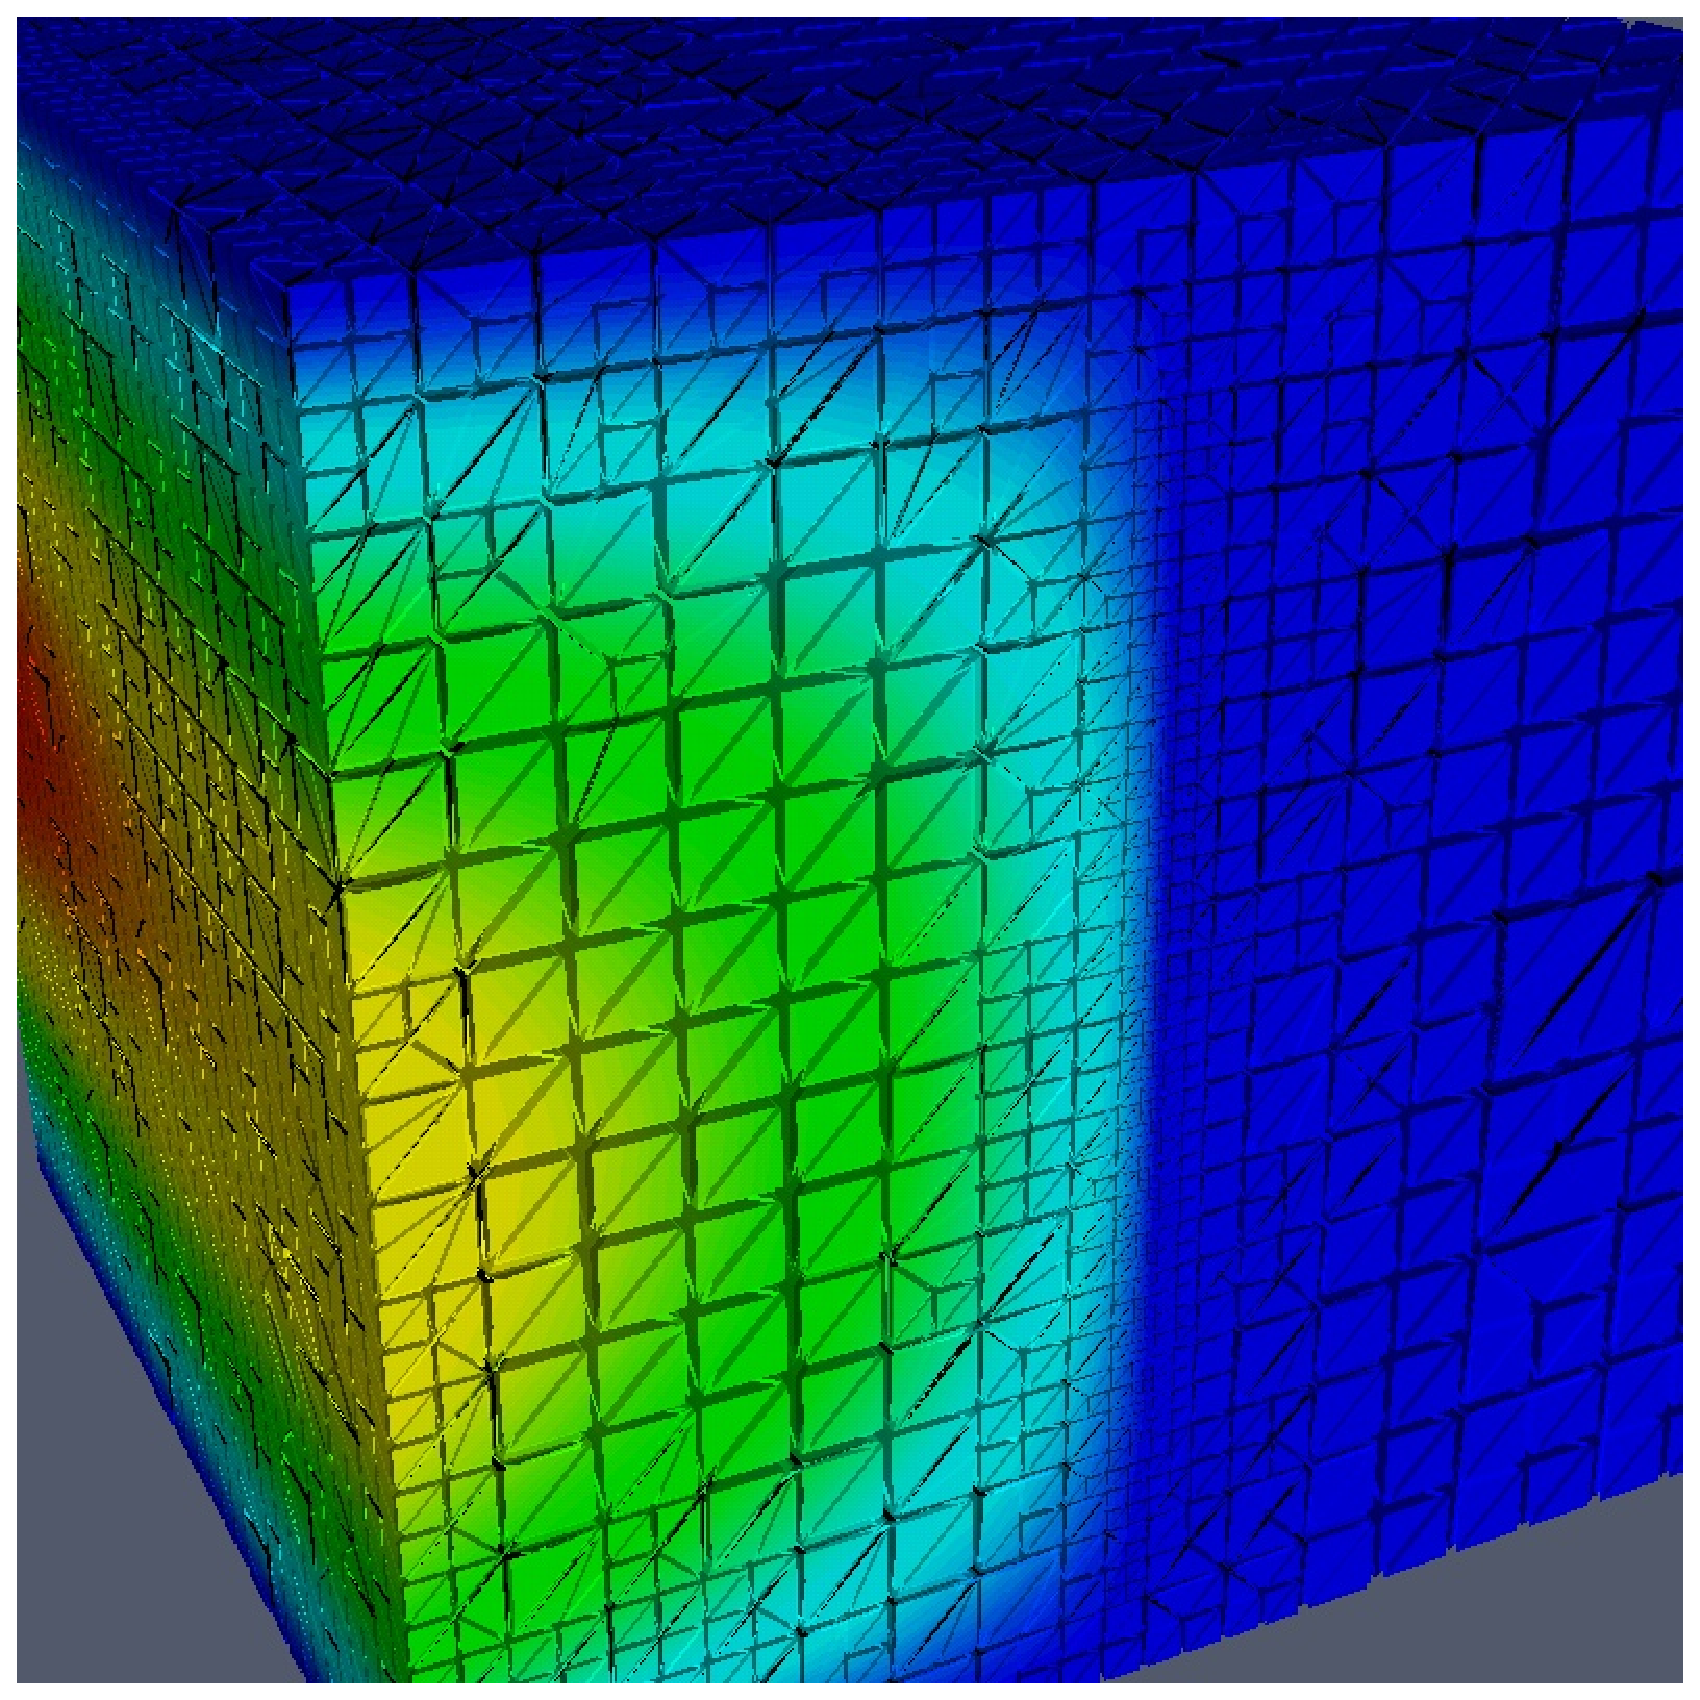
\includegraphics[width=0.32\textwidth]{EPS/ugsimplex3d}\
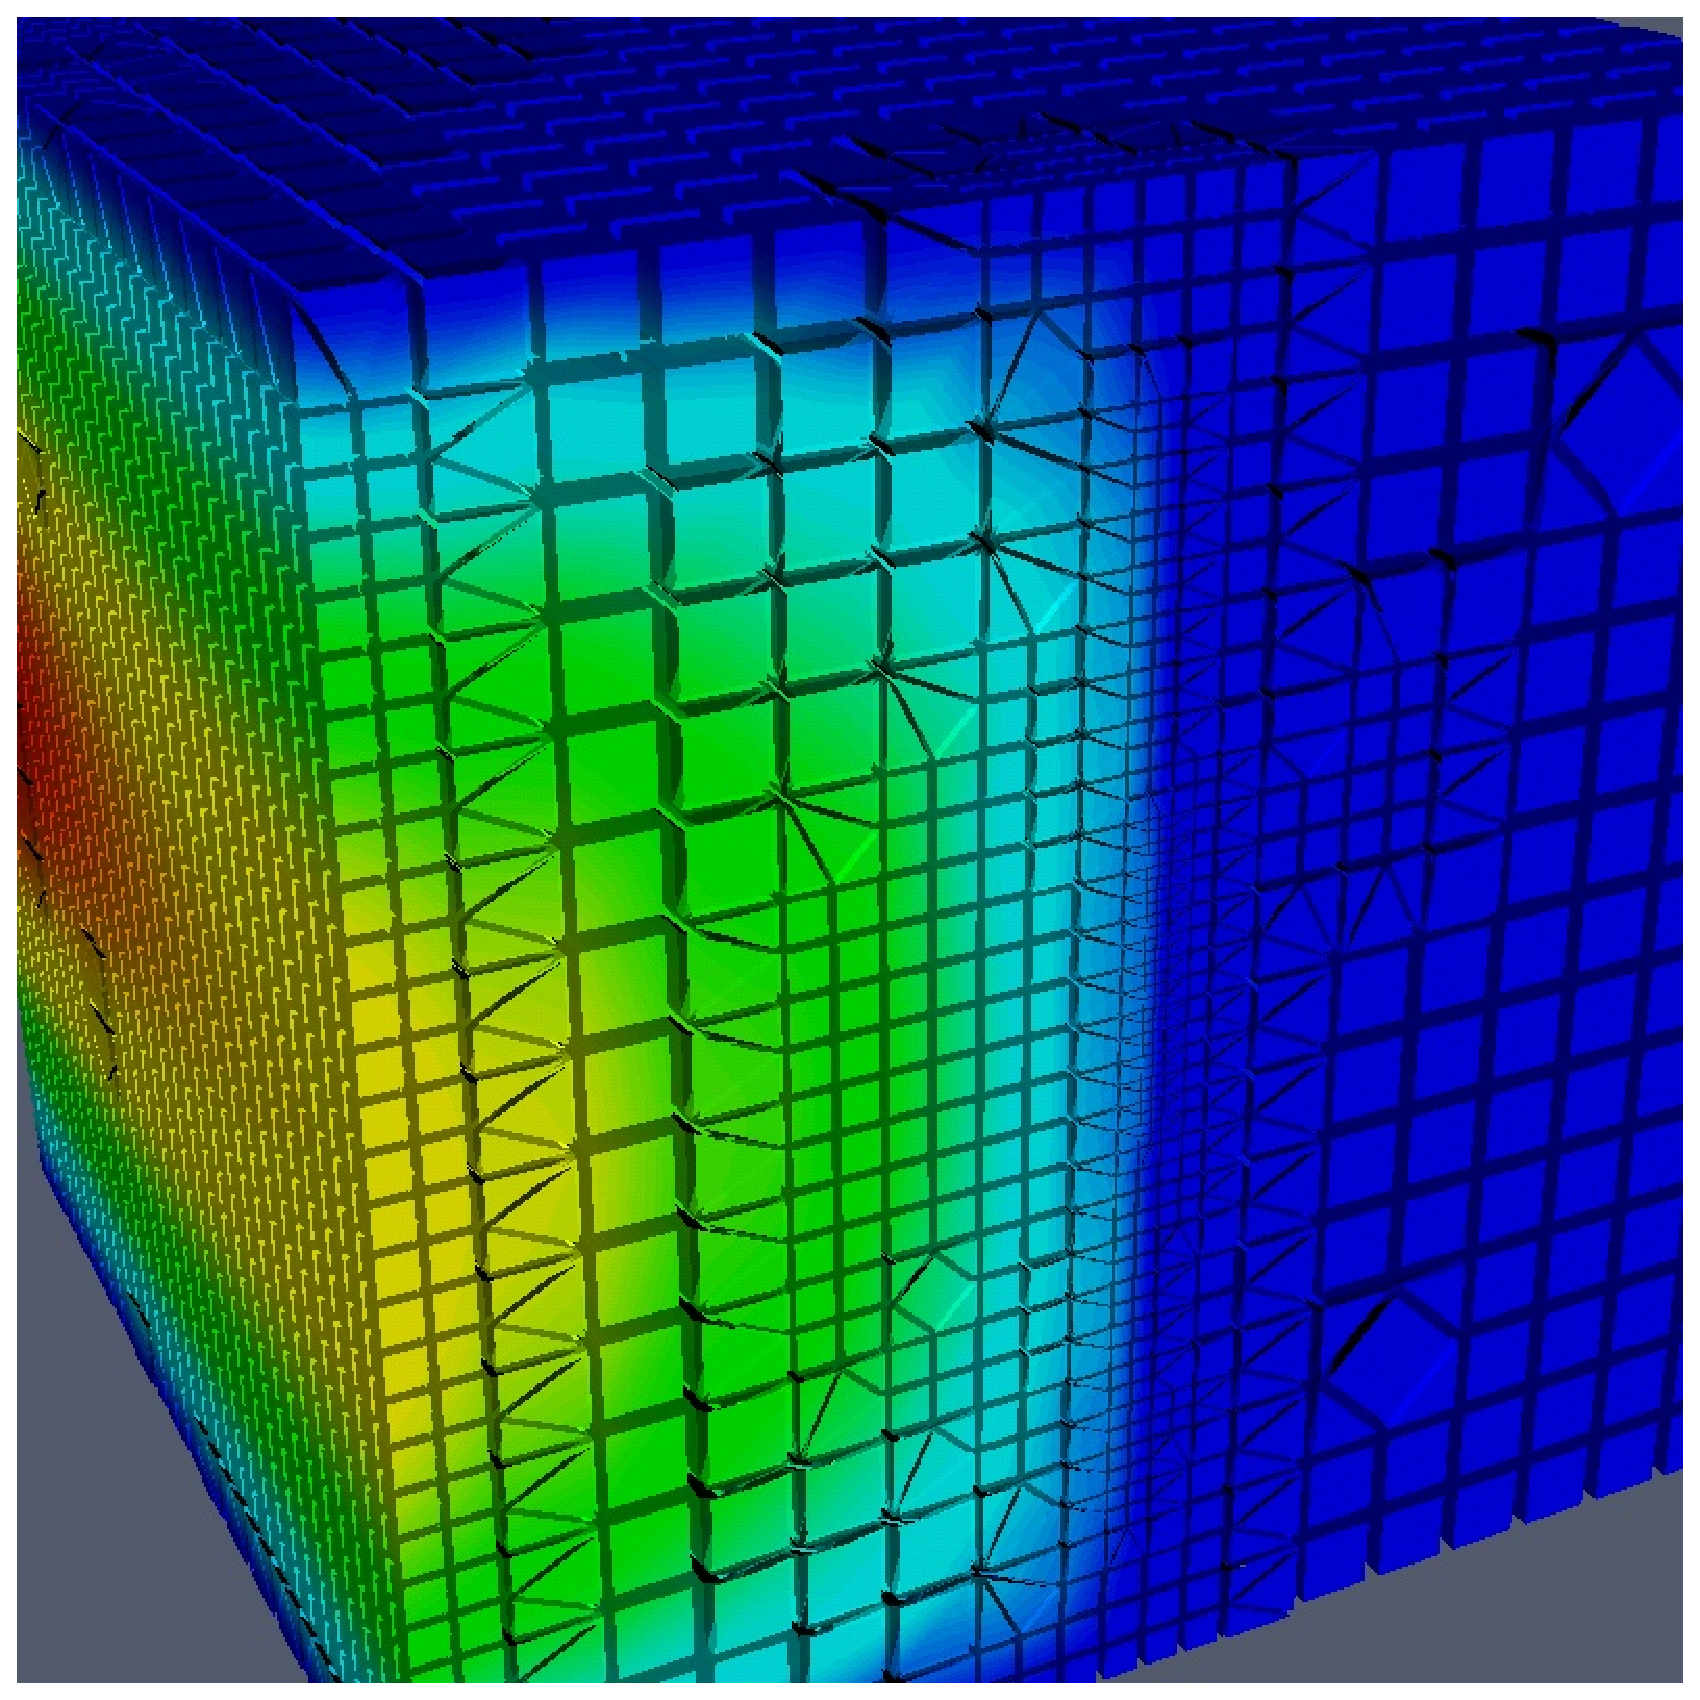
\includegraphics[width=0.32\textwidth]{EPS/ugcube3d}\
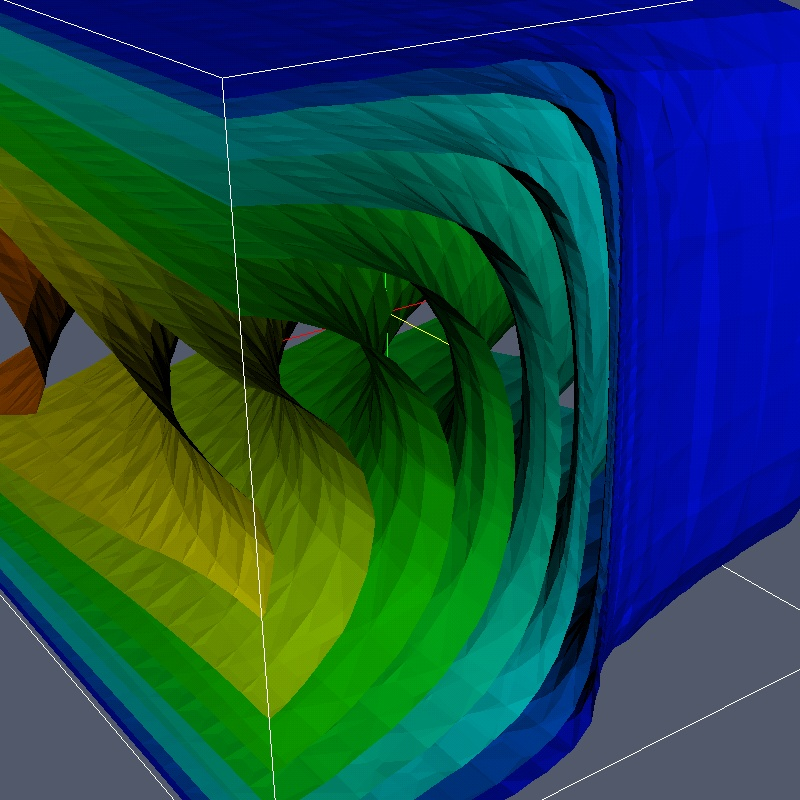
\includegraphics[width=0.32\textwidth]{EPS/iso}

\caption{Adaptive solution of an elliptic model problem with $P_1$
conforming finite elements and residual based error
estimator. Illustrates that adaptive finite element algorithm can be formulated
independent of dimension, element type and refinement scheme. From
top to bottom, left to right: Alberta (bisection, 2d), UG (red/green
on triangles), UG (red/green on quadrilaterals), Alberta (bisection,
3d), ALU (hanging nodes on tetrahedra), ALU (hanging nodes on
hexahedra), UG (red/green on tetrahedra), UG (red/green on hexahedra,
pyramids and tetrahedra), isosurfaces of solution.}
\label{Fig:OutlookP1}
\end{figure}



\bibliographystyle{plain}
\bibliography{grid-howto.bib}

\end{document}
